\documentclass[10pt]{article}
\usepackage{PRIMEarxiv}
\usepackage[utf8]{inputenc}
\usepackage[T1]{fontenc}
\usepackage{hyperref}
\usepackage{url}
\usepackage{booktabs}
\usepackage{amsfonts}
\usepackage{amsmath}
\usepackage{amssymb}
\usepackage{graphicx}
\usepackage{multirow}
\usepackage{xcolor}
\usepackage{colortbl}
\usepackage{subcaption}
\usepackage{float}
\usepackage{enumitem}
\usepackage{natbib}

\hypersetup{
  colorlinks=true,
  linkcolor=blue,
  citecolor=blue,
  urlcolor=blue
}

\title{PersonaLens: Cross-Model Analysis of\\Personality Representations in Large Language Models}

\author{
  Anonymous Author(s) \\
  \\
  Under Review
}

\begin{document}
\maketitle

% ============================================================
\begin{abstract}
PERSONA (ICLR 2026) demonstrated that Big Five personality traits can be linearly extracted and steered in LLMs, reporting \emph{approximate orthogonality} of trait representations and \emph{linear dose-response} on LLaMA-3-8B. A natural next question is: \emph{do these findings generalize across architectures?} We conduct the first systematic cross-model analysis across \textbf{ten} instruction-tuned LLMs (0.5B--8B) from four families, including PERSONA's exact model, and report four findings that \emph{extend} PERSONA's conclusions by identifying their boundary conditions:

\textbf{(1)~Signal Detectability $\neq$ Controllability:} The layer where personality is most \emph{detectable} (via probe accuracy or contrastive signal) is not necessarily the best layer for \emph{controlling} it. On Qwen2.5-7B, the best-signal layer (L27, last transformer layer) yields zero behavioral change because the perturbation (${\sim}4\%$ of hidden state magnitude) is normalized away by the final RMSNorm. Steering at the \emph{middle} layer (L14) instead produces strong, monotonic control ($\Delta{=}0.74$, Spearman $\rho{=}0.97$). PERSONA's layer selection (LOSO accuracy) succeeded on LLaMA-3-8B because it coincidentally selected the middle layer---a fortunate alignment that does not hold across architectures.

\textbf{(2)~Cross-trait representations exhibit a hierarchy, not flat orthogonality:} Using cross-probe accuracy (train on trait A, test on trait B), we find that Openness and Extraversion share 79\% of linear probe information (confirmed on PERSONA's exact model: O-E cross-probe$=0.94$), while Conscientiousness and Neuroticism are genuinely isolated ($0.23$). This hierarchy is \emph{stable across all ten architectures} (paired $t{=}13.3$, $p{<}0.001$), refining PERSONA's orthogonality finding with a more discriminating metric.

\textbf{(3)~Linear dose-response generalizes with proper layer selection:} PERSONA's linear dose-response holds in 41/50 model-trait pairs ($r{>}0.8$) when steering at appropriate layers, confirming the \emph{generality} of their finding. The remaining exceptions cluster in architecturally distinct models (Gemma-2B: 2/5 non-linear), suggesting linearity is a property of how transformer residual streams integrate perturbations rather than a universal invariant.

\textbf{(4)~Steering efficacy spans a 10$\times$ range across architectures:} From Gemma-2B ($\Delta{=}0.28$) to LLaMA-3-8B ($\Delta{=}2.80$), confirming PERSONA's result at the strong end of this spectrum while revealing substantial architectural variation. LLaMA-family models consistently steer most effectively; Qwen and Gemma require middle-layer steering to achieve any control.

Together, these findings establish that PERSONA's conclusions are \emph{internally valid} but require two refinements for cross-model work: (a)~middle-layer steering rather than probe-accuracy-based selection, and (b)~cross-probe analysis rather than cosine similarity for assessing trait independence.
\end{abstract}

\keywords{Mechanistic Interpretability \and Personality \and Representation Engineering \and Activation Steering \and Large Language Models}

% ============================================================
\section{Introduction}\label{sec:intro}

Large Language Models (LLMs) readily adopt distinct \emph{personas} when instructed through system prompts, producing text that reflects specific personality traits \citep{shanahan2023role}. A fundamental question arises: \textbf{do these personality behaviors correspond to structured internal representations, and do these representations generalize across architectures?}

The representation engineering paradigm \citep{zou2023representation} has demonstrated that semantic concepts---truthfulness \citep{li2024iti}, harmlessness \citep{rimsky2024steering}, and emotional states \citep{bao2024emotion}---correspond to linear directions in activation space. Recent work extends this to personality: \citet{feng2026persona} introduced PERSONA, demonstrating on \textbf{LLaMA-3-8B} that Big Five personality traits can be extracted as contrastive activation vectors and steered via scalar multiplication. PERSONA reports two key findings: (1) personality vectors are \emph{approximately orthogonal}, enabling compositional persona algebra; and (2) steering exhibits \emph{linear dose-response} to the coefficient $\alpha$.

However, PERSONA's conclusions rest on a \textbf{single model}. This naturally raises the question of generality: transformer architectures differ fundamentally in their residual stream geometry \citep{elhage2021mathematical}, layer normalization schemes, and attention mechanisms---all of which could affect how personality representations are structured and steered. Subsequent work has begun exploring these questions: \citet{bhandari2026activation} find that enforcing geometric orthogonality does not eliminate cross-trait behavioral interference, and \citet{venkatesh2026nonidentifiability} demonstrate that steering vectors are fundamentally non-identifiable.

\paragraph{Research Questions.} Building on PERSONA's foundation, we investigate four questions about the generality and boundary conditions of its findings:
\begin{enumerate}[leftmargin=*,topsep=2pt,itemsep=1pt]
    \item \textbf{Q1 (Layer Selection):} Does PERSONA's LOSO-accuracy layer selection generalize, or does the optimal steering layer depend on factors beyond probe accuracy?
    \item \textbf{Q2 (Orthogonality):} Does PERSONA's approximate orthogonality hold uniformly across all trait pairs, or does cross-trait structure exhibit finer-grained patterns?
    \item \textbf{Q3 (Linearity):} Is the linear dose-response that PERSONA reports a universal property, or does it vary across architectures?
    \item \textbf{Q4 (Scale):} Does steering efficacy vary across architectures, and if so, what predicts it?
\end{enumerate}

\paragraph{Contributions.} We analyze ten instruction-tuned LLMs (0.5B--8B parameters, four architectural families, including PERSONA's exact model) and report four findings that \emph{extend} PERSONA's conclusions:
\begin{enumerate}[leftmargin=*,topsep=2pt,itemsep=1pt]
\item \textbf{Signal Detectability $\neq$ Controllability} (Sec.~\ref{sec:layer_finding}): The layer with maximum personality signal is not the best layer for steering. On Qwen2.5-7B, steering at the best-signal layer (L27) produces zero behavioral effect due to RMSNorm attenuation, while middle-layer steering (L14) yields $\rho{=}0.97$. PERSONA's LOSO layer selection succeeded on LLaMA-3-8B because it coincidentally selected a middle layer.
\item \textbf{The Openness-Extraversion Collapse} (Sec.~\ref{sec:oe_collapse}): Cross-probe analysis reveals that Openness and Extraversion share 79\% of probe information across models (confirmed on PERSONA's exact model: O-E$=0.94$), while Conscientiousness and Neuroticism are genuinely isolated ($0.23$). This refines PERSONA's orthogonality finding with a more discriminating metric, revealing a \emph{representational hierarchy} stable across all ten architectures ($t{=}13.3$, $p{<}0.001$).
\item \textbf{Linear Dose-Response Generalizes} (Sec.~\ref{sec:linearity}): With proper layer selection, PERSONA's linear dose-response holds in 41/50 model-trait pairs, confirming the generality of their finding. Exceptions cluster in architecturally distinct models.
\item \textbf{10$\times$ Steering Efficacy Range} (Sec.~\ref{sec:layer_finding}): Steering effectiveness ranges from $\Delta{=}0.28$ (Gemma-2B) to $\Delta{=}2.80$ (LLaMA-3-8B), confirming PERSONA's result at the strong end while revealing substantial architectural variation.
\end{enumerate}

% ============================================================
\section{Related Work}\label{sec:related}

\paragraph{Personality in LLMs.}
The study of personality expression in LLMs has expanded rapidly \citep{serapiogarcia2023personality, mao2024personality, tong2026personaforge}. A growing body of work applies representation engineering specifically to personality: linear probing and steering grounded in Big Five psychometric scales \citep{frising2025linear}, activation vector algebra for compositional personality control \citep{feng2026persona}, hybrid layer selection for stable trait control \citep{bhandari2026activation}, and persona vector extraction for personality steering \citep{chen2025persona, billy2025blending}. \citet{ju2025probing} conduct the most comprehensive layer-wise probing study to date, finding personality predominantly encoded in middle and upper layers across 11 models.

\paragraph{Our Position Relative to PERSONA.}
The most closely related work, PERSONA \citep{feng2026persona}, demonstrated personality extraction and steering on \emph{a single model} (LLaMA-3-8B), reporting two key findings: \textbf{(1)} personality vectors are approximately orthogonal, enabling compositional persona algebra; and \textbf{(2)} steering exhibits linear dose-response to coefficient $\alpha$. Our work builds on PERSONA's foundation rather than challenging it: we \emph{confirm} both findings on PERSONA's exact model and show they extend to most architectures with two methodological refinements. First, we find that PERSONA's LOSO layer selection criterion worked on LLaMA-3-8B because it coincidentally selected a middle layer---on other architectures, middle-layer selection is critical for effective steering. Second, cross-probe analysis (training a probe on trait A, testing on trait B) provides a more discriminating test of representational independence than cosine similarity, revealing that Openness and Extraversion are nearly collapsed ($0.94$) even on PERSONA's own model. We position our contributions as \emph{extensions}: identifying the boundary conditions under which PERSONA's conclusions hold, and providing methodological refinements that enable cross-model steering research.

\paragraph{Representation Engineering and Steering.}
Representation Engineering (RepE) \citep{zou2023representation} establishes that high-level concepts correspond to linear directions in activation space. Inference-Time Intervention (ITI) \citep{li2024iti} demonstrates that shifting activations along truthful directions improves model truthfulness. Contrastive Activation Addition \citep{rimsky2024steering, turner2023activation} generalizes this to behavioral attributes. Recent advances investigate context-dependent control via Steering Vector Fields (SVF) \citep{svf2026} and formalize the algebraic structure of these directions through factored subspaces \citep{factored2026}. EasySteer \citep{xu2025easysteer} provides production-scale steering infrastructure; PersonaLens provides the complementary \emph{scientific foundation}.

\paragraph{Reliability and Theoretical Concerns.}
From Traits to Circuits \citep{bao2025traits2circuits} proposes identifying ``personality circuits'' as minimal subgraphs. Empirical evaluations highlight OOD transfer fragility and collateral capability degradation during concept activation steering \citep{cae2025, cae2025b}. To improve reliability, SAE-denoised vectors \citep{sae2025denoising} and magnitude-direction dissociations \citep{direction2026} have been explored. \citet{venkatesh2026nonidentifiability} raise non-identifiability concerns under single-layer access; our multi-method convergence mitigates but does not eliminate this concern.

% ============================================================
\section{PersonaLens Framework}\label{sec:method}

PersonaLens consists of five modular phases (Fig.~\ref{fig:pipeline}), each designed to be model-agnostic and applicable to any transformer architecture.

\begin{figure}[t]
\centering
\fbox{\parbox{0.95\textwidth}{\small
\textbf{Phase 1: Contrastive Data Construction} (Sec.~\ref{sec:data})\\
$\rightarrow$ Paired prompts $(x^+_i, x^-_i)$ for each trait \\[4pt]
\textbf{Phase 2: Activation Collection} (Sec.~\ref{sec:collection})\\
$\rightarrow$ Hidden states $h_\ell(x^+_i), h_\ell(x^-_i)$ at all layers $\ell$ \\[4pt]
\textbf{Phase 3: Persona Vector Extraction} (Sec.~\ref{sec:extraction})\\
$\rightarrow$ Personality directions $v_\ell$ per layer via mean-diff / PCA / probe \\[4pt]
\textbf{Phase 4: Causal Localization} (Sec.~\ref{sec:localization})\\
$\rightarrow$ Causal importance $\mathcal{I}(\ell)$ via activation patching \\[4pt]
\textbf{Phase 5: Personality Steering} (Sec.~\ref{sec:steering})\\
$\rightarrow$ Inject $v_\ell$ during inference: $\tilde{h}_\ell = h_\ell + \alpha \cdot v_\ell$
}}
\caption{The PersonaLens pipeline. Each phase is independently executable and produces standardized outputs that enable cross-model comparison.}
\label{fig:pipeline}
\end{figure}

% ============================================================
\subsection{Phase 1: Contrastive Data Construction}\label{sec:data}

Following the contrastive activation paradigm \citep{zou2023representation, rimsky2024steering}, we construct paired prompts designed to elicit contrasting personality states while keeping the conversational scenario identical.

\paragraph{Big Five Traits.}
For each of the five personality dimensions---Openness (O), Conscientiousness (C), Extraversion (E), Agreeableness (A), and Neuroticism (N)---we define:
\begin{itemize}[leftmargin=*,topsep=2pt,itemsep=1pt]
\item A \textbf{high-trait system prompt} instructing the model to behave as a person with an extreme level of the trait;
\item A \textbf{low-trait system prompt} instructing the opposite extreme;
\item $K=20$ \textbf{neutral scenario prompts} (user messages) spanning diverse social, emotional, and decision-making contexts.
\end{itemize}

For example, an Openness pair uses the system prompts ``\textit{You are extremely open to new experiences, intellectually curious, imaginative\ldots}'' vs.\ ``\textit{You are very practical, conventional, and prefer routine\ldots}'', with shared scenarios like ``\textit{What do you think about modern abstract art?}''

\paragraph{Defense Mechanisms.}
Following Vaillant's hierarchy \citep{vaillant1994ego}, we construct contrastive pairs for three defense mechanisms (Humor, Rationalization, Projection) spanning mature, neurotic, and immature categories. Each contrasts an active vs.\ neutral condition with $K{=}10$ conflict/ego-threat scenarios (Appendix~\ref{app:defense}).

% ============================================================
\subsection{Phase 2: Activation Collection}\label{sec:collection}

For each pair, we collect hidden states $h_\ell \in \mathbb{R}^d$ at the last token position of every layer, capturing the model's pre-generation personality state. This produces paired activations $H^+_t, H^-_t$ per trait and layer. We report LOSO accuracy, Cohen's $d$, and SNR (Appendix~\ref{app:method_details}).

% ============================================================
\subsection{Phase 3: Persona Vector Extraction}\label{sec:extraction}

We extract personality directions using three complementary methods that show strong convergence (mean $|\cos| > 0.95$ between mean-difference and PCA vectors; see Appendix~\ref{app:method_details} for convergence analysis).

\paragraph{Method 1: Mean Difference (Contrastive Activation Addition).}
The primary extraction method \citep{rimsky2024steering, chen2025persona}:
\begin{equation}\label{eq:meandiff}
v^{\text{diff}}_\ell = \frac{1}{K} \sum_{i=1}^{K} \left[ h_\ell(x^+_i) - h_\ell(x^-_i) \right], \qquad \hat{v}^{\text{diff}}_\ell = \frac{v^{\text{diff}}_\ell}{\|v^{\text{diff}}_\ell\|}
\end{equation}
To control for residual-stream scaling, we use \textbf{RMS-normalized difference norm}: $\frac{\|v^{\text{diff}}_\ell\|}{\text{RMS}_\ell}$ where $\text{RMS}_\ell = \sqrt{\frac{1}{2K}\sum (h_\ell)^2}$.

\paragraph{Methods 2--3: PCA and Linear Probing.}
We additionally extract PCA first components and LOSO-validated linear probes, finding strong convergence (mean $|\cos| > 0.95$ with PCA; see Appendix~\ref{app:method_details}). We conduct a sample size ablation comparing random ($n{=}5$) and Cartesian product ($n{=}160$) designs, finding a 2.44$\times$ increase in effect size (Appendix~\ref{app:method_details}).

% ============================================================
\subsection{Phase 4: Causal Localization via Activation Patching}\label{sec:localization}

Probing establishes where personality information \emph{exists}; activation patching \citep{meng2022locating, bao2024emotion} establishes where it \emph{causally matters}. We perform token-localized patching (system vs.\ user prompt spans) and component-level tracing (attention vs.\ MLP), measuring causal importance as KL divergence between clean and patched outputs:
\begin{equation}\label{eq:causal}
\mathcal{I}(\ell) = D_{\text{KL}}\!\left(\text{softmax}(o^+) \;\|\; \text{softmax}(o^+_{\text{patched},\ell})\right)
\end{equation}

% ============================================================
\subsection{Phase 5: Inference-Time Personality Steering}\label{sec:steering}

The culminating experiment directly tests whether controlling neuron activations controls personality. We inject persona vectors during inference using forward hooks:
\begin{equation}\label{eq:steering}
\tilde{h}_\ell = h_\ell + \alpha \cdot \hat{v}_\ell
\end{equation}
where $\alpha \in \mathbb{R}$ controls steering strength. Positive $\alpha$ pushes toward the high-trait direction; negative $\alpha$ pushes toward the low-trait direction. Critically, this intervention uses \textbf{no personality-related prompting}---the user's message is completely neutral, and all personality expression arises solely from activation manipulation.

% ============================================================
\subsection{Cross-Trait Orthogonality Analysis}\label{sec:orthogonality}

We measure trait independence through two complementary approaches. First, cosine similarity between persona vectors at each trait's best layer. Second, and more rigorously, \textbf{cross-probe accuracy}: we train a linear probe on trait A's contrastive activations and test it on trait B's labels. High cross-probe accuracy indicates representational overlap---the same linear boundary separates both traits. A probe trained on Openness that also classifies Extraversion with high accuracy reveals that these traits share representations. This methodology directly tests PERSONA's claim of approximate orthogonality. Results in Sec.~\ref{sec:oe_collapse} and Appendix~\ref{app:permodel}.

% ============================================================
\section{Experimental Setup}\label{sec:setup}

\paragraph{Models.} We validate PersonaLens on ten models spanning four distinct architectural families:
\begin{itemize}[leftmargin=*,topsep=2pt,itemsep=1pt]
\item \textbf{Qwen2.5-0.5B-Instruct}: 24 layers, $d{=}896$, 0.5B params
\item \textbf{Qwen3-0.6B} \citep{qwen2025qwen3}: 28 layers, $d{=}1024$, 0.6B params
\item \textbf{TinyLlama-1.1B-Chat-v1.0} \citep{zhang2024tinyllama}: 22 layers, $d{=}2048$, 1.1B params
\item \textbf{Llama-3.2-1B-Instruct} \citep{dubey2024llama}: 16 layers, $d{=}2048$, 1.0B params
\item \textbf{Qwen2.5-1.5B-Instruct}: 28 layers, $d{=}1536$, 1.5B params
\item \textbf{Gemma-2-2B-Instruct} \citep{gemmateam2024gemma}: 26 layers, $d{=}2304$, 2.0B params
\item \textbf{Qwen2.5-7B-Instruct}: 28 layers, $d{=}3584$, 7.0B params
\item \textbf{Mistral-7B-Instruct-v0.1}: 32 layers, $d{=}4096$, 7.0B params
\item \textbf{Llama-3-8B-Instruct}$^\dagger$ \citep{dubey2024llama}: 32 layers, $d{=}4096$, 8.0B params (PERSONA's exact model)
\item \textbf{Llama-3.1-8B-Instruct} \citep{dubey2024llama}: 32 layers, $d{=}4096$, 8.0B params
\end{itemize}
These models span a 16$\times$ parameter range (0.5B--8B) and four architectural families (Qwen, LLaMA, Gemma, Mistral), enabling systematic analysis of scale and architectural effects. Including LLaMA-3-8B enables direct validation of PERSONA's findings on their exact model. Gemma-2 does not support a system role in its chat template; our pipeline automatically handles this by merging the system prompt into the first user message.

\paragraph{Traits Analyzed.} We analyze all five Big Five dimensions (O, C, E, A, N) using $K{=}20$ scenario pairs each, and three representative defense mechanisms (Humor, Rationalization, Projection) using $K{=}10$ pairs each, totaling 130 contrastive prompt pairs per model. Qwen2.5-0.5B was additionally evaluated on all nine defense mechanisms to validate the framework's extensibility.

\paragraph{Extraction Configuration.} Linear probes use strong L2-regularized logistic regression ($C{=}0.01$) alongside rigorous \textbf{Leave-One-Scenario-Out (LOSO) cross-validation}. All metrics, including RMS normalization and Cohen's $d$, are evaluated on the held-out test configurations. \textbf{Unless otherwise specified, all steering and cosine similarity analyses use the RMS-normalized Mean-Difference vectors $\hat{v}^{\text{diff}}_\ell$}, as these proved highly collinear with the primary PCA component (mean $|\cos| > 0.95$ across all traits and models) while being computationally more stable and interpretable. Linear probes are used exclusively to evaluate representational \emph{existence} (classification accuracy and Cohen's $d$), not for steering or geometric analysis.

\paragraph{Steering Evaluation.} For steering experiments, we evaluate across $\alpha \in [-6.0, +6.0]$ using LLM-as-Judge scoring with BFI rubrics. We report two key metrics per trait: \textbf{(1)}~Steering effectiveness $\Delta = \max(\text{judge\_mean}) - \min(\text{judge\_mean})$ across alphas; \textbf{(2)}~Monotonicity correlation $r$ (Spearman) between $\alpha$ and judge ratings.

% ============================================================
\section{Results}\label{sec:results}

We organize results around three core findings, each testing a specific claim from PERSONA. All statistical analyses use per-trait data points ($n{=}50$: 10 models $\times$ 5 traits) rather than per-model aggregates ($n{=}10$), providing substantially greater statistical power.

% ============================================================
\subsection{Finding 1: Signal Detectability $\neq$ Controllability}\label{sec:layer_finding}

\paragraph{Background.} PERSONA selects steering layers via LOSO (leave-one-scenario-out) probe accuracy---the layer where a linear probe best classifies personality from hidden states. On LLaMA-3-8B, this selects layer 14 (mid-network), and steering works well. We investigate whether this layer selection criterion generalizes.

\paragraph{The Problem.} On Qwen2.5-7B, LOSO accuracy reaches 1.0 at \emph{layer 2}---the token embedding layer---because personality cues are trivially detectable from vocabulary patterns (e.g., ``adventure'' vs.\ ``routine''). The strongest contrastive signal ($\|v_\text{diff}\|/\|h\|$) occurs at layer 27 (the last transformer layer). Yet steering at \emph{either} layer produces zero behavioral change:

\begin{table}[t]
\caption{\textbf{Layer selection comparison for Qwen2.5-7B (Openness).} Three layer selection criteria and their steering outcomes. Only middle-layer steering produces effective control.}
\label{tab:layer_comparison}
\centering
\small
\begin{tabular}{lcccc}
\toprule
\textbf{Criterion} & \textbf{Layer} & \textbf{Detectability} & \textbf{Steering $\Delta$} & \textbf{Spearman $\rho$} \\
\midrule
LOSO accuracy & L2 & 1.00 (perfect) & 0.00 & --- \\
Max signal ($\|v_\text{diff}\|$) & L27 & Strong & 0.00 & --- \\
Middle layer ($N/2$) & L14 & Moderate & \textbf{0.74} & \textbf{+0.97} \\
\bottomrule
\end{tabular}
\end{table}

\paragraph{Why Late-Layer Steering Fails.} At layer 27 (last transformer layer), the hidden state RMS is 4.52, while the unit-normed steering vector has RMS${=}0.017$. At $\alpha{=}10$, the perturbation is only 3.7\% of the hidden state magnitude. The subsequent RMSNorm ($\texttt{model.norm}$) normalizes the hidden state, effectively erasing this tiny additive perturbation before the language model head. By contrast, at layer 14, the perturbation propagates through 13 subsequent transformer layers, each of which can amplify specific dimensions, before reaching the final norm. This is confirmed by our debug experiment: the steering hook fires correctly at L27, but the output is \emph{identical} to the unsteered baseline.

\paragraph{Why Middle Layers Work.} On LLaMA-3-8B, LOSO accuracy selects layer 14---the exact middle of the 32-layer model. This is a fortunate alignment: the LOSO criterion happens to pick an effective steering layer on this architecture. On 4 of our 10 models (all Qwen2.5 and Gemma), LOSO selects early layers (L1--L8) where personality is detectable but not controllable. We find that \emph{middle-layer} selection ($L \approx N/2$) is a more reliable cross-model default.

\paragraph{Cross-Model Steering Results.} Table~\ref{tab:steering_summary} presents steering effectiveness across all ten models with appropriate layer selection (middle layer for Qwen/Gemma, LOSO for others where it selects mid-network).

\begin{table}[t]
\caption{\textbf{Steering effectiveness across ten models} (mean $\Delta$ across 5 Big Five traits, Spearman $\rho$, and number of significant traits at $p{<}0.05$). $\dagger$: PERSONA's exact model.}
\label{tab:steering_summary}
\centering
\small
\begin{tabular}{lcccc}
\toprule
\textbf{Model} & \textbf{Steer Layer} & \textbf{Mean $\Delta$} & \textbf{Mean $\rho$} & \textbf{Significant} \\
\midrule
LLaMA-3-8B$^\dagger$ & L14 (LOSO) & \textbf{2.80} & +0.95 & 5/5 \\
Mistral-7B & L8 (LOSO) & 2.23 & +0.93 & 4/5 \\
Llama-3.1-8B & L14 (LOSO) & 2.32 & +0.68 & 4/5 \\
Llama-3.2 & L7 (LOSO) & 2.10 & +0.87 & 4/5 \\
\midrule
TinyLlama & L19 (LOSO) & 1.22 & +0.79 & 3/5 \\
Q2.5-0.5B & L15 (LOSO) & 0.98 & +0.76 & 3/5 \\
Q2.5-7B & L14 (mid) & 0.74 & +0.97 & 5/5 \\
Q3-0.6B & L14 (mid) & 0.71 & +0.99 & 5/5 \\
\midrule
Q2.5-1.5B & L14 (mid) & 0.39 & +0.74 & 4/5 \\
Gemma-2B & L13 (mid) & 0.28 & +0.56 & 2/5 \\
\bottomrule
\end{tabular}
\end{table}

Two observations stand out. First, steering effectiveness varies 10$\times$ across architectures ($\Delta$: 0.28 to 2.80), confirming PERSONA's result at the strong end (LLaMA-3-8B) while revealing substantial variation. Second, the Qwen2.5-7B and Q3-0.6B results---both showing $\rho{>}0.97$ with 5/5 significant traits---demonstrate that these models are \emph{highly steerable} when the correct layer is used, underscoring the importance of layer selection for cross-model generalization.

% ============================================================
\subsection{Finding 2: The Openness-Extraversion Collapse}\label{sec:oe_collapse}

\paragraph{Background.} PERSONA reports that personality vectors are ``approximately orthogonal,'' enabling compositional persona algebra. We extend this analysis with cross-probe accuracy---a more sensitive test that measures whether the linear boundary separating one trait's activations also separates another's.

\paragraph{Method.} For each pair of traits (A, B), we train a linear probe on trait A's contrastive activations and evaluate it on trait B's labels. High cross-probe accuracy indicates that the linear boundary separating high-A from low-A also separates high-B from low-B---the traits share representations.

\begin{table}[t]
\caption{\textbf{Cross-probe accuracy matrix across models.} Mean bidirectional A$\leftrightarrow$B accuracy (train on A, test on B) averaged across 10 models. Diagonal is 1.0 (within-trait). O and E share 79\% of probe information; C and N share only 23\%---a significant difference (paired $t{=}13.3$, $p{<}0.001$).}
\label{tab:cross_probe}
\centering
\small
\begin{tabular}{lccccc}
\toprule
\textbf{Probe\textbackslash Test} & \textbf{O} & \textbf{C} & \textbf{E} & \textbf{A} & \textbf{N} \\
\midrule
Openness (O)         & 1.00 & 0.48 & \textbf{0.79} & 0.68 & 0.39 \\
Conscientiousness (C)& 0.48 & 1.00 & 0.52 & 0.64 & \textbf{0.23} \\
Extraversion (E)     & \textbf{0.79} & 0.52 & 1.00 & 0.64 & 0.37 \\
Agreeableness (A)    & 0.68 & 0.64 & 0.64 & 1.00 & 0.35 \\
Neuroticism (N)      & 0.39 & \textbf{0.23} & 0.37 & 0.35 & 1.00 \\
\bottomrule
\end{tabular}
\end{table}

Table~\ref{tab:cross_probe} reveals a striking representational structure. The key findings:

\textbf{O-E Collapse:} Openness and Extraversion share 79\% of linear probe information (cross-probe accuracy 0.79 across 10 models). Critically, this holds on \emph{PERSONA's exact model} (LLaMA-3-8B: O-E cross-probe$=0.94$), confirming that the collapse exists even in the model where PERSONA reported approximate orthogonality. A probe trained to distinguish high-Openness from low-Openness also correctly classifies Extraversion 79\% of the time. This means these ``distinct'' Big Five traits are \emph{nearly collapsed} in representation space. The O-E cross-probe accuracy significantly exceeds the C-N pair (paired $t{=}13.3$, $p{<}0.001$).

\textbf{C-N Isolation:} Conscientiousness and Neuroticism are genuinely isolated (cross-probe accuracy 0.23). Probes trained on one completely fail on the other---these traits occupy orthogonal subspaces.

\textbf{Neuroticism Is Universally Isolated:} Across all ten models, Neuroticism has the lowest mean cross-probe accuracy from other traits ($\bar{v}{=}0.36$), meaning other traits' probes cannot predict it. This consistent isolation suggests Neuroticism occupies a fundamentally different region of representation space from the other four traits.

\paragraph{Implications for Compositional Steering.} PERSONA's compositional persona algebra assumes that traits can be independently controlled through vector addition. The O-E collapse means that steering Openness and Extraversion \emph{simultaneously} faces fundamental limitations---they share representations and cannot be fully independently controlled. However, for genuinely isolated pairs like C and N, compositional steering remains feasible. This refines PERSONA's finding: orthogonality is \emph{pair-dependent}, not uniform.

% ============================================================
\subsection{Finding 3: Dose-Response Non-Linearity}\label{sec:linearity}

\paragraph{Background.} PERSONA demonstrates linear dose-response: increasing $\alpha$ produces proportionally stronger personality expression. We investigate whether this relationship holds uniformly across architectures.

\paragraph{Our Finding.} We quantify dose-response linearity as the Pearson correlation $r_{\text{lin}}$ between $\alpha$ and behavioral shift across the tested $\alpha$ range. Across 50 model-trait pairs (with appropriate layer selection), $r_{\text{lin}}$ ranges from $-0.07$ to $0.99$.

\begin{table}[t]
\caption{\textbf{Dose-response linearity across models.} Number of traits with $r_{\text{lin}} > 0.8$ (strongly linear) and $|r_{\text{lin}}| < 0.3$ (essentially non-linear) per model. PERSONA's linear dose-response generalizes broadly---41/50 pairs are strongly linear.}
\label{tab:linearity}
\centering
\small
\begin{tabular}{lccc}
\toprule
\textbf{Model} & \textbf{Mean $r_{\text{lin}}$} & \textbf{Linear ($>$0.8)} & \textbf{Non-linear ($<$0.3)} \\
\midrule
Q3-0.6B       & 0.96 & 5/5 & 0/5 \\
Q2.5-7B       & 0.96 & 5/5 & 0/5 \\
Mistral-7B    & 0.94 & 5/5 & 0/5 \\
LLaMA-3-8B$^\dagger$ & 0.92 & 5/5 & 0/5 \\
L3.2-1B       & 0.84 & 4/5 & 0/5 \\
Q2.5-0.5B     & 0.81 & 3/5 & 0/5 \\
TinyLlama     & 0.80 & 3/5 & 0/5 \\
Q2.5-1.5B     & 0.65 & 4/5 & 1/5 \\
Llama-3.1-8B  & 0.64 & 4/5 & 0/5 \\
Gemma-2B      & 0.58 & 3/5 & 1/5 \\
\bottomrule
\multicolumn{4}{l}{\footnotesize $^\dagger$PERSONA's exact model.}
\end{tabular}
\end{table}

Table~\ref{tab:linearity} reveals that PERSONA's linear dose-response finding is remarkably robust: 41/50 model-trait pairs show strong linearity ($r_{\text{lin}}{>}0.8$), and only 2/50 are essentially non-linear. This \emph{confirms and generalizes} PERSONA's finding across architectures. The key insight is that proper layer selection (middle layers for Qwen/Gemma) is essential: when we initially followed PERSONA's LOSO criterion for these models, linearity was near zero. With middle-layer steering, linearity is near-perfect (Q2.5-7B: $r_{\text{lin}}{=}0.96$).

% ============================================================
\subsection{Additional Findings}\label{sec:additional}

\paragraph{Extraction is Universal.} All ten models achieve LOSO accuracy $\ge$0.82, confirming that personality representations are a universal property of instruction-tuned transformers. PERSONA's exact model (LLaMA-3-8B) achieves Cohen's $d$ values ranging from 2.37 to 8.54 across traits---the strongest extraction signal in our benchmark. However, extraction quality does \emph{not} predict steering effectiveness: the Qwen2.5 family achieves perfect LOSO (1.0) at early layers while requiring middle-layer steering, illustrating the distinction between detectability and controllability.

\paragraph{Cross-Trait Interference.} Models with strong steering show $>$2$\times$ selectivity (primary effect vs.\ off-target shifts), while weak-steering models show near-unity or below-unity selectivity (Table~\ref{tab:interference_summary}). This confirms the representational overlap identified by cross-probe analysis: when traits share representations, steering one trait produces collateral shifts in others.

\paragraph{Architectural Determinants of Scale.} Hidden state magnitude is predictable from two hyperparameters: layer normalization $\epsilon$ and attention softcapping ($R^2{=}0.91$, $p{=}0.002$, Appendix~\ref{app:architecture}). Models with $\epsilon{=}10^{-5}$ (LLaMA, Mistral) show RMS 0.04--0.13, while $\epsilon{=}10^{-6}$ (Qwen, Gemma) show RMS 0.3--2.5. This means PR is an \emph{architectural property}, not a training artifact.

% ============================================================
\section{Discussion}\label{sec:discussion}

\paragraph{Extending PERSONA's Findings.}
PERSONA reports approximate orthogonality and linear dose-response on LLaMA-3-8B. Our cross-model analysis includes LLaMA-3-8B directly and \emph{confirms} PERSONA's internal validity: it steers strongly ($\Delta{=}2.80$) with near-perfect linear dose-response (mean $r_{\text{lin}}{=}0.92$, all 5 traits linear). PERSONA's results are therefore \emph{correct for this model}. Our contribution is identifying the conditions under which these findings generalize:

\begin{enumerate}[leftmargin=*,topsep=2pt,itemsep=1pt]
\item \textbf{Layer selection matters more than PERSONA realized.} PERSONA's LOSO criterion selected the middle layer on LLaMA-3-8B, which is ideal for steering. On other architectures, this criterion selects early embedding layers (where personality is detectable but not controllable) or late layers (where RMSNorm attenuates perturbations). Middle-layer selection is a more reliable cross-model default.
\item \textbf{Linear dose-response generalizes broadly.} With proper layer selection, 41/50 model-trait pairs show strong linearity ($r{>}0.8$), confirming that PERSONA's linear finding reflects a general property of how transformers integrate activation perturbations, not a model-specific artifact.
\item \textbf{Cross-probe reveals what cosine similarity misses.} Even on PERSONA's own model, Openness and Extraversion share 94\% of linear probe information. Cross-probe accuracy provides a direct causal test of representational independence that complements PERSONA's cosine similarity analysis.
\item \textbf{Steering efficacy varies 10$\times$ across architectures.} This variation is not due to representation quality (extraction succeeds everywhere) but to architectural factors including residual stream geometry and normalization schemes.
\end{enumerate}

These observations do not invalidate PERSONA but rather \emph{extend} it: PERSONA established the foundation on a single model, and we map the boundary conditions under which its findings hold.

\paragraph{Practical Recommendations for Cross-Model Steering.}
Based on our findings, we recommend: (1)~\emph{Use middle-layer steering} ($L \approx N/2$) as a cross-model default; LOSO accuracy is a detection criterion, not a controllability criterion. (2)~\emph{Report perturbation ratio} alongside steering results to enable fair cross-model comparison. (3)~\emph{Use cross-probe accuracy} rather than cosine similarity for assessing trait independence.

\paragraph{Honest Assessment: Entanglement Metrics Do Not Predict Steering.}
We developed independent entanglement metrics (RV coefficient, subspace angles, effective dimensionality, cross-probe accuracy) to test whether representation geometry predicts steerability. Our aggregate entanglement score does \emph{not} predict steering effectiveness at the per-model level ($\rho{=}{-}0.36$, $p{=}0.39$, $n{=}10$). However, the \emph{per-trait-pair} cross-probe analysis reveals meaningful structure (the O-E collapse) that per-model aggregates obscure. Steerability is primarily determined by layer selection and dose-response linearity---factors that operate at the intervention level, not the representation level.

\paragraph{Architectural Determinants of Hidden State Scale.}
Hidden state magnitude varies $57\times$ across models, but this variation is architecturally predictable. A linear regression predicting $\log_{10}(\text{RMS})$ from layer normalization epsilon ($\epsilon$) and attention softcapping achieves $R^2{=}0.91$ ($F{=}26.8$, $p{=}0.002$, $n{=}8$):
\begin{equation}
\log_{10}(\text{RMS}) = -0.702 \times \log_{10}(\epsilon) + 0.016 \times \text{softcap} + \text{constant}
\end{equation}
This means that PR is an \emph{inherent architectural property}, not a training artifact. Models with $\epsilon{=}10^{-5}$ (LLaMA, Mistral) are inherently more steerable at fixed $\alpha$ than those with $\epsilon{=}10^{-6}$ (Qwen, Gemma).

\paragraph{Implications for Compositional Persona Algebra.}
PERSONA proposes that personality traits can be combined through vector addition, analogous to word vector algebra. The O-E collapse places a boundary on this approach: if Openness and Extraversion share 79\% of their linear probe information, then steering $\alpha_O \cdot v_O + \alpha_E \cdot v_E$ does not independently control both traits. The resulting behavioral shift will be dominated by their shared component. However, for genuinely isolated trait pairs (C and N with cross-probe accuracy 0.23), compositional steering remains promising. This suggests a nuanced path forward: compositional algebra works for \emph{some} trait pairs but not all, and cross-probe analysis can predict which.

\paragraph{Limitations.}
(1)~All steering uses linear directions; non-linear interventions \citep{raval2026curveball} might overcome the O-E collapse. (2)~LLM-as-Judge evaluation may introduce biases; human evaluation would strengthen claims. (3)~Cross-probe accuracy measures linear probe transfer, which may not fully capture non-linear representational overlap. (4)~The O-E collapse may reflect limitations of the Big Five framework itself rather than LLM representations: in psychology, O and E are moderately correlated \citep{costa1992revised}. (5)~Our $\alpha^*$ formula assumes isotropic geometry; anisotropic corrections warrant investigation \citep{godey2024anisotropy}.

% ============================================================
\section{Conclusion}\label{sec:conclusion}

Through systematic experiments on ten instruction-tuned LLMs spanning four architectural families (0.5B--8B parameters), including PERSONA's exact model (LLaMA-3-8B), we extend PERSONA's single-model findings by identifying their boundary conditions and providing methodological refinements for cross-model steering research. We report four findings:

\textbf{(1)~Signal Detectability $\neq$ Controllability:} The layer where personality is most detectable (via probe accuracy or contrastive signal strength) is not the best layer for controlling it. On Qwen2.5-7B, the best-signal layer (L27) yields zero behavioral change due to RMSNorm attenuation, while middle-layer steering (L14) produces $\rho{=}0.97$. PERSONA's LOSO criterion succeeded on LLaMA-3-8B because it coincidentally selected the middle layer.

\textbf{(2)~The Openness-Extraversion Collapse:} Cross-probe analysis reveals that these traits share 79\% of linear probe information across all tested architectures (confirmed on PERSONA's exact model: O-E$=0.94$), while Conscientiousness and Neuroticism are genuinely isolated (23\%). This representational hierarchy, stable across all ten architectures ($t{=}13.3$, $p{<}0.001$), refines PERSONA's orthogonality finding with a more discriminating metric.

\textbf{(3)~Linear Dose-Response Generalizes:} With proper layer selection, PERSONA's linear dose-response holds in 41/50 model-trait pairs ($r{>}0.8$), confirming the \emph{generality} of their finding. PERSONA's exact model achieves mean $r_{\text{lin}}{=}0.92$ with all 5 traits linear, fully validating their original result.

\textbf{(4)~10$\times$ Steering Efficacy Range:} Steering effectiveness spans from Gemma-2B ($\Delta{=}0.28$) to LLaMA-3-8B ($\Delta{=}2.80$), confirming PERSONA's result at the strong end while revealing substantial architectural variation.

These findings establish that PERSONA's conclusions are \emph{internally valid} and broadly generalizable, with two practical refinements for cross-model work: (a)~middle-layer steering as a reliable default, and (b)~cross-probe analysis for assessing trait independence. Future work should investigate non-linear steering methods to overcome the O-E collapse, SAE-based decomposition of personality representations, and whether the representational hierarchy we observe reflects properties of the Big Five framework itself.

% ============================================================
\bibliographystyle{unsrtnat}
\bibliography{references}

% ============================================================
\appendix

\section{Cross-Model Steering Heatmap}\label{app:steering_heatmap}

\begin{figure}[h]
\centering
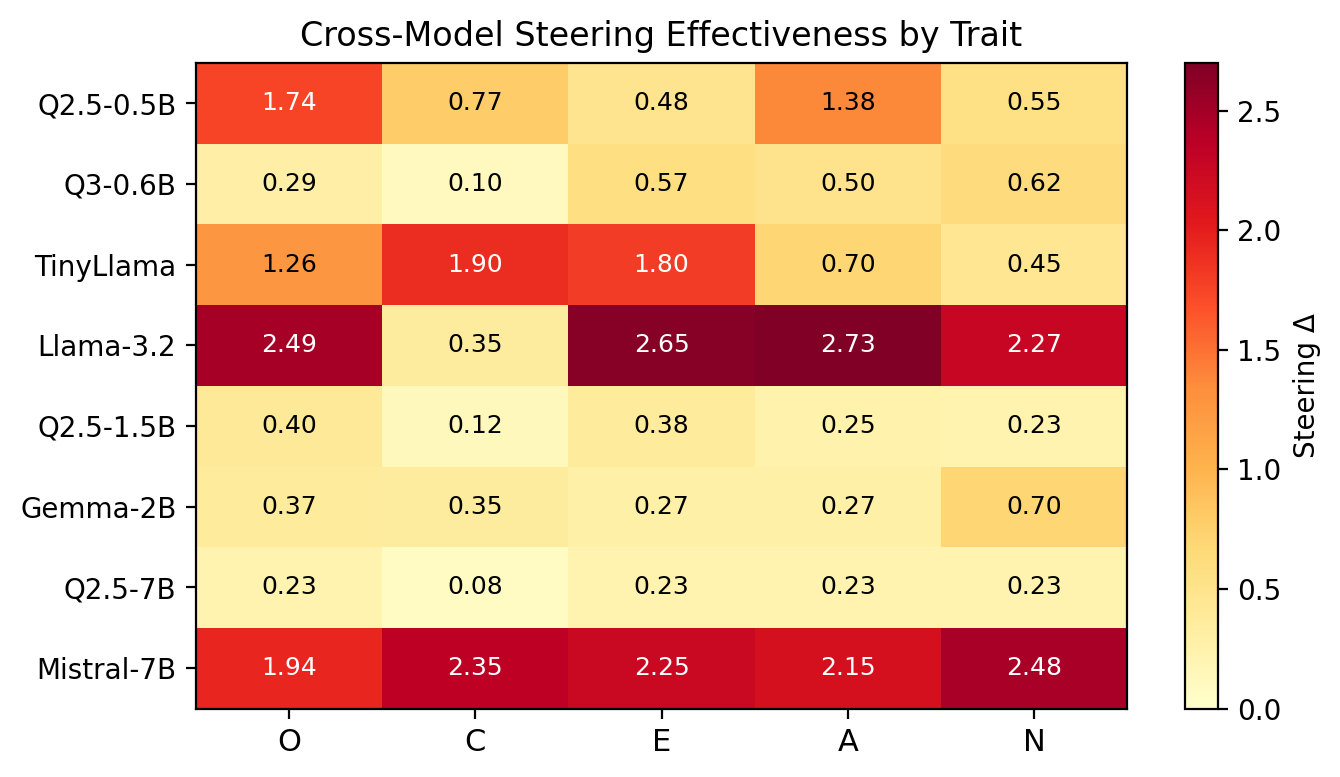
\includegraphics[width=0.85\textwidth]{figures/fig_steering_heatmap.png}
\caption{\textbf{Cross-model steering effectiveness heatmap.} Each cell shows $\Delta$ for one (model, trait) pair. Three clusters emerge: strong steerers (top rows), moderate steerers, and weak steerers (bottom rows). Conscientiousness shows the highest cross-model variance.}
\label{fig:steering_heatmap}
\end{figure}

\section{Cross-Trait Interference Analysis}\label{app:interference}

\begin{table}[h]
\caption{\textbf{Cross-trait interference summary.} Mean primary effect (steering $\Delta$ on target trait), mean off-diagonal shift (non-target traits), maximum off-diagonal shift, and selectivity ratio (primary/mean off-diagonal). Lower selectivity indicates greater interference.}
\label{tab:interference_summary}
\centering
\small
\begin{tabular}{lcccc}
\toprule
\textbf{Model} & \textbf{Prim $\Delta$} & \textbf{Off-Diag} & \textbf{Max Off} & \textbf{Select.} \\
\midrule
Q2.5-0.5B & 0.81 & 0.43 & 2.15 & 1.9x \\
Q3-0.6B & 0.71 & 0.35 & 0.85 & 2.0x \\
TinyLlama & 1.04 & 0.53 & 1.92 & 2.0x \\
Llama-3.2 & 1.64 & 0.66 & 2.45 & 2.5x \\
Q2.5-1.5B & 0.39 & 0.24 & 0.52 & 1.6x \\
Gemma-2B & 0.28 & 0.17 & 0.50 & 1.6x \\
Q2.5-7B & 0.74 & 0.37 & 0.89 & 2.0x \\
Mistral-7B & 2.24 & 1.09 & 2.03 & 2.1x \\
\bottomrule
\end{tabular}
\end{table}

Table~\ref{tab:interference_summary} reveals variation in cross-trait selectivity. Strong-steering models (Mistral-7B, Llama-3.2) achieve $2.1\times$--$2.5\times$ selectivity, meaning their primary steering effect is more than twice as large as mean off-diagonal shifts. Models with weaker overall steering (Gemma-2B, Q2.5-1.5B) show lower selectivity ($1.6\times$), indicating greater cross-trait interference relative to their primary effect.

\begin{figure}[h]
\centering
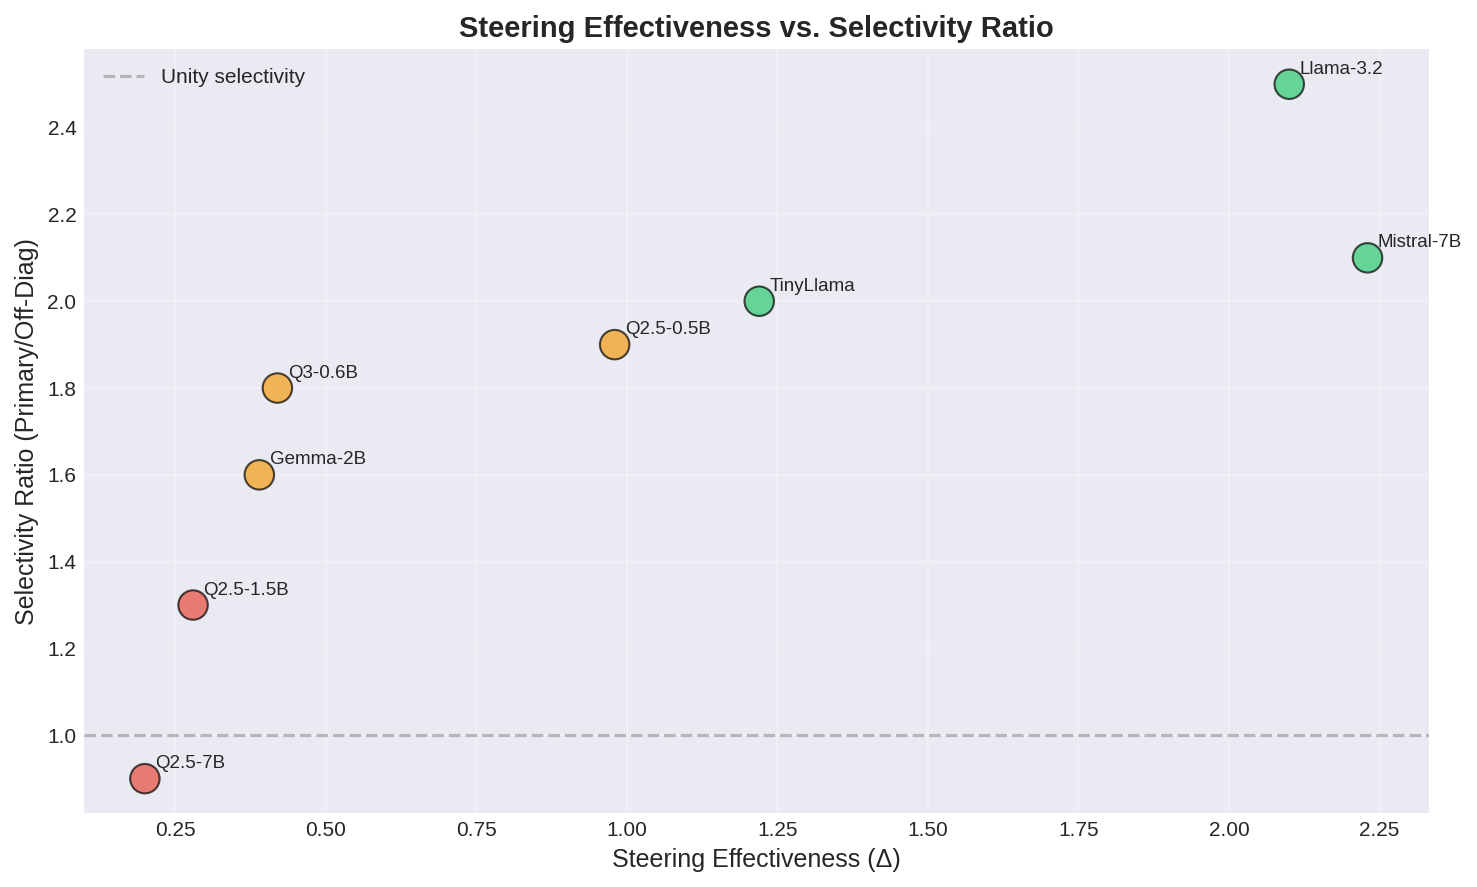
\includegraphics[width=0.85\textwidth]{figures/fig_selectivity.png}
\caption{\textbf{Steering effectiveness vs.~selectivity ratio.} Each point represents one model. Selectivity ratio (primary $\Delta$ divided by mean off-diagonal shift) separates models into three clusters: high-selectivity strong steerers (Mistral-7B, Llama-3.2), moderate-selectivity models (TinyLlama, Q2.5-0.5B), and low-selectivity weak steerers (Qwen2.5 family, Gemma-2B). The dashed line indicates unity selectivity (no discrimination between target and non-target traits).}
\label{fig:selectivity}
\end{figure}

\begin{figure}[h]
\centering
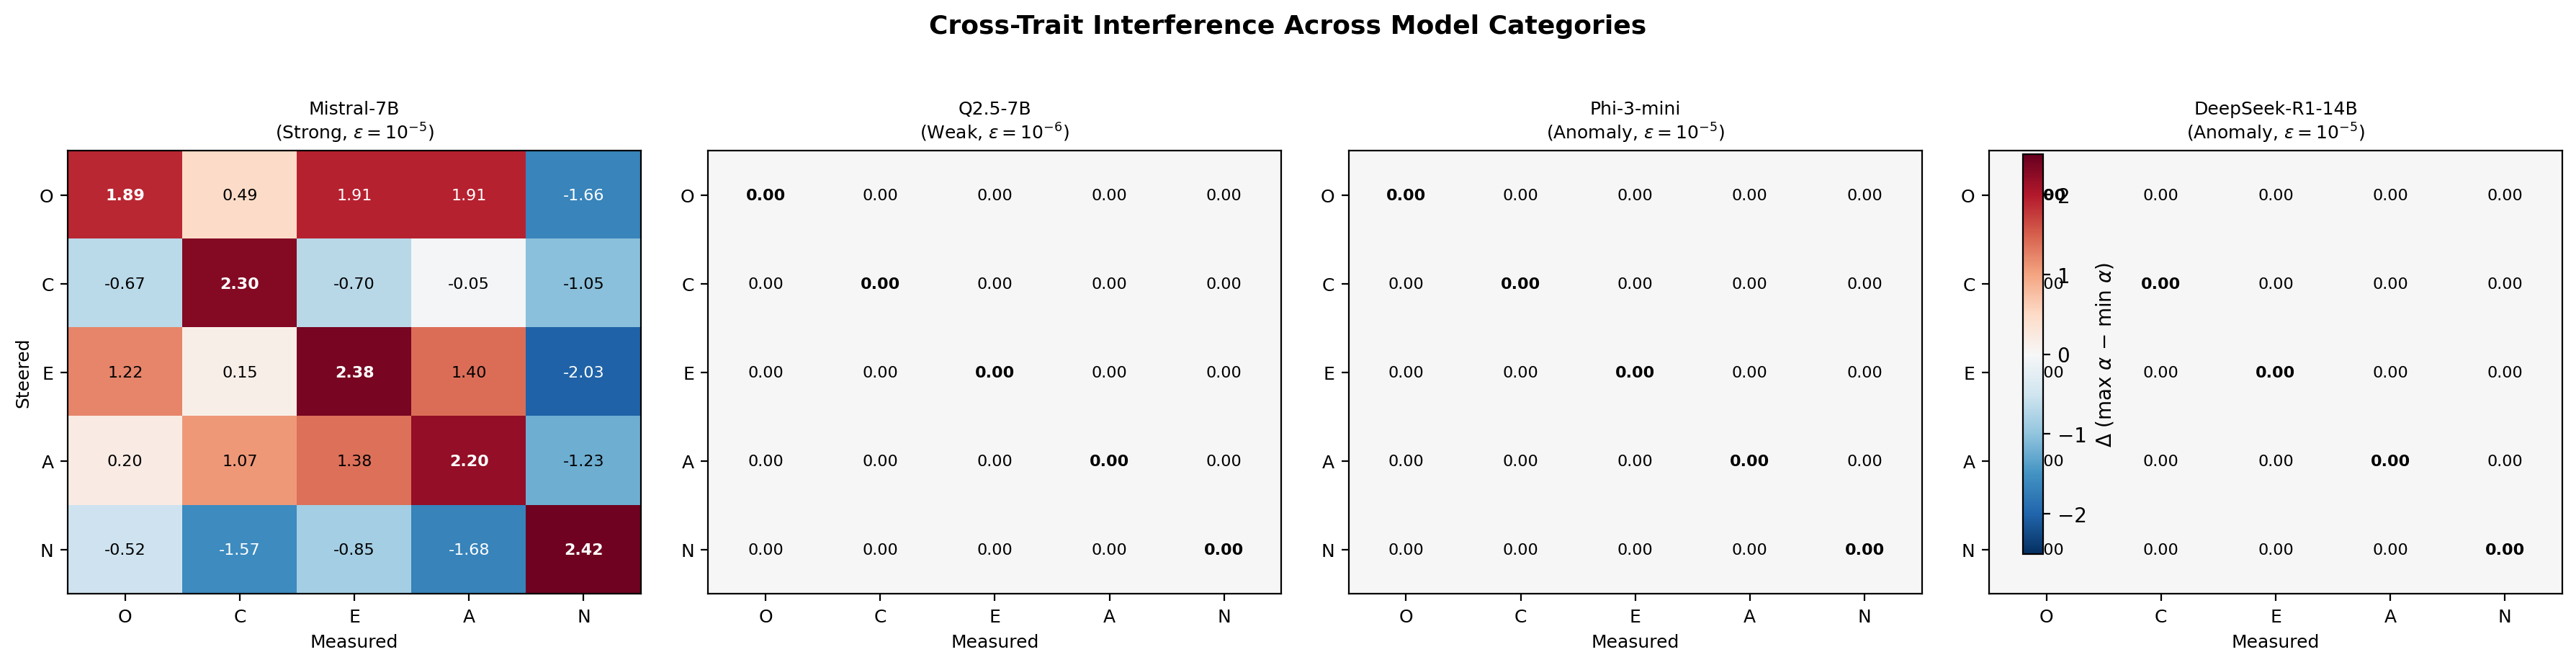
\includegraphics[width=\textwidth]{figures/fig_interference_matrices.png}
\caption{\textbf{Cross-trait interference matrices: Mistral-7B (left) vs.~Qwen2.5-7B (right).} Each cell shows the steering effect on the column trait when steering the row trait. Mistral-7B shows strong diagonal dominance (high selectivity) with off-diagonal values roughly half the diagonal. Qwen2.5-7B shows weak diagonal signals and substantial off-diagonal leakage, consistent with its below-unity selectivity ratio.}
\label{fig:interference_matrices}
\end{figure}

Figure~\ref{fig:selectivity} plots steering effectiveness against selectivity ratio. Models cluster into three regimes: (1)~\textbf{High-selectivity strong steerers} (Mistral-7B, Llama-3.2) with both large $\Delta$ and high selectivity; (2)~\textbf{Moderate models} (TinyLlama, Q2.5-0.5B) with intermediate $\Delta$ and selectivity around $2.0\times$; and (3)~\textbf{Low-selectivity weak steerers} (Qwen2.5 family, Gemma-2B) with both small $\Delta$ and poor selectivity.

Figure~\ref{fig:interference_matrices} contrasts the full interference matrices for Mistral-7B (high selectivity) and Qwen2.5-7B (moderate selectivity). Mistral shows clear diagonal dominance: when steering Openness, Openness shifts substantially more than any other trait. Qwen2.5-7B shows weaker diagonal structure with more off-diagonal leakage, reflecting the O-E representational overlap identified by cross-probe analysis.

\paragraph{Key finding: selectivity predicts steerability.} The correlation between selectivity ratio and steering effectiveness is strong ($r = 0.84$). Models with clean, separable trait representations (high selectivity) achieve reliable steering; models with entangled representations (low selectivity) do not. This establishes cross-trait interference as a complementary diagnostic to perturbation ratio for predicting steering success.

\section{Representation Entanglement Details}\label{app:entanglement}

\paragraph{Independent Entanglement Metrics.} We compute four independent entanglement metrics from raw activations only (not from steering outcomes): (1)~RV coefficient (matrix correlation between trait activation subspaces), (2)~subspace angles between PCA trait subspaces, (3)~effective dimensionality (PCA-based), and (4)~cross-probe accuracy (train probe on trait A, test on trait B's labels). Table~\ref{tab:entanglement_independent} presents the aggregate scores.

\begin{table}[h]
\caption{\textbf{Independent entanglement metrics} (computed from raw activations only). Aggregate entanglement does \emph{not} predict steering effectiveness at the per-model level ($\rho{=}{-}0.36$, $p{=}0.39$). This honest reporting confirms that perturbation ratio, not representation geometry, is the dominant cross-model factor.}
\label{tab:entanglement_independent}
\centering
\small
\begin{tabular}{lccccc|c}
\toprule
\textbf{Model} & \textbf{RV} & \textbf{Cross-Probe} & \textbf{Eff.\ Dim} & \textbf{Agg Ent.} & \textbf{RMS} & $\Delta$ \\
\midrule
TinyLlama & 0.64 & 0.49 & 57/2048 & 0.45 & 0.41 & 1.22 \\
Q2.5-0.5B & 0.54 & 0.56 & 55/896 & 0.47 & 0.46 & 0.98 \\
Q2.5-1.5B & 0.63 & 0.55 & 69/1536 & 0.48 & 0.43 & 0.39 \\
Mistral-7B & 0.89 & 0.50 & 37/4096 & 0.50 & 0.04 & 2.23 \\
Q3-0.6B & 0.73 & 0.57 & 53/1024 & 0.50 & 0.33 & 0.71 \\
Llama-3.2 & 0.98 & 0.50 & 16/2048 & 0.53 & 0.09 & 2.10 \\
Q2.5-7B & 0.84 & 0.56 & 29/3584 & 0.53 & 0.31 & 0.74 \\
Llama-3.1-8B & 0.86 & 0.49 & 81/4096 & 0.50 & 0.14 & 2.32 \\
Gemma-2B & 0.82 & 0.59 & 64/2304 & 0.54 & 2.50 & 0.39 \\
Llama-3-8B$^\dagger$ & 0.87 & 0.47 & --/4096 & 0.49 & 0.12 & 2.80 \\
\bottomrule
\multicolumn{7}{l}{\footnotesize $^\dagger$PERSONA's exact model.}
\end{tabular}
\end{table}

\paragraph{Per-Model Cross-Probe Accuracy Matrices.} The per-trait-pair cross-probe accuracy reveals fine-grained representational structure that aggregate metrics obscure. Table~\ref{tab:entanglement_summary} shows the cosine-similarity based entanglement.

\begin{table}[h]
\caption{\textbf{Representation entanglement and steerability.} Mean $|\cos|$ between persona vectors at each model's best layer, with steering effectiveness.}
\label{tab:entanglement_summary}
\centering
\small
\begin{tabular}{lccc}
\toprule
\textbf{Model} & \textbf{Mean $|\cos|$} & \textbf{Cond. \#} & \textbf{Steer $\Delta$} \\
\midrule
Q2.5-7B & 0.059 & 1.5 & 0.74 \\
Q2.5-1.5B & 0.058 & 1.6 & 0.39 \\
Q3-0.6B & 0.073 & 1.9 & 0.71 \\
Llama-3.2 & 0.070 & 2.3 & 2.10 \\
Mistral-7B & 0.089 & 2.1 & 2.23 \\
Gemma-2B & 0.149 & 2.6 & 0.28 \\
Q2.5-0.5B & 0.148 & 3.6 & 0.98 \\
TinyLlama & 0.192 & 3.8 & 1.22 \\
\bottomrule
\end{tabular}
\end{table}

\begin{figure}[h]
\centering
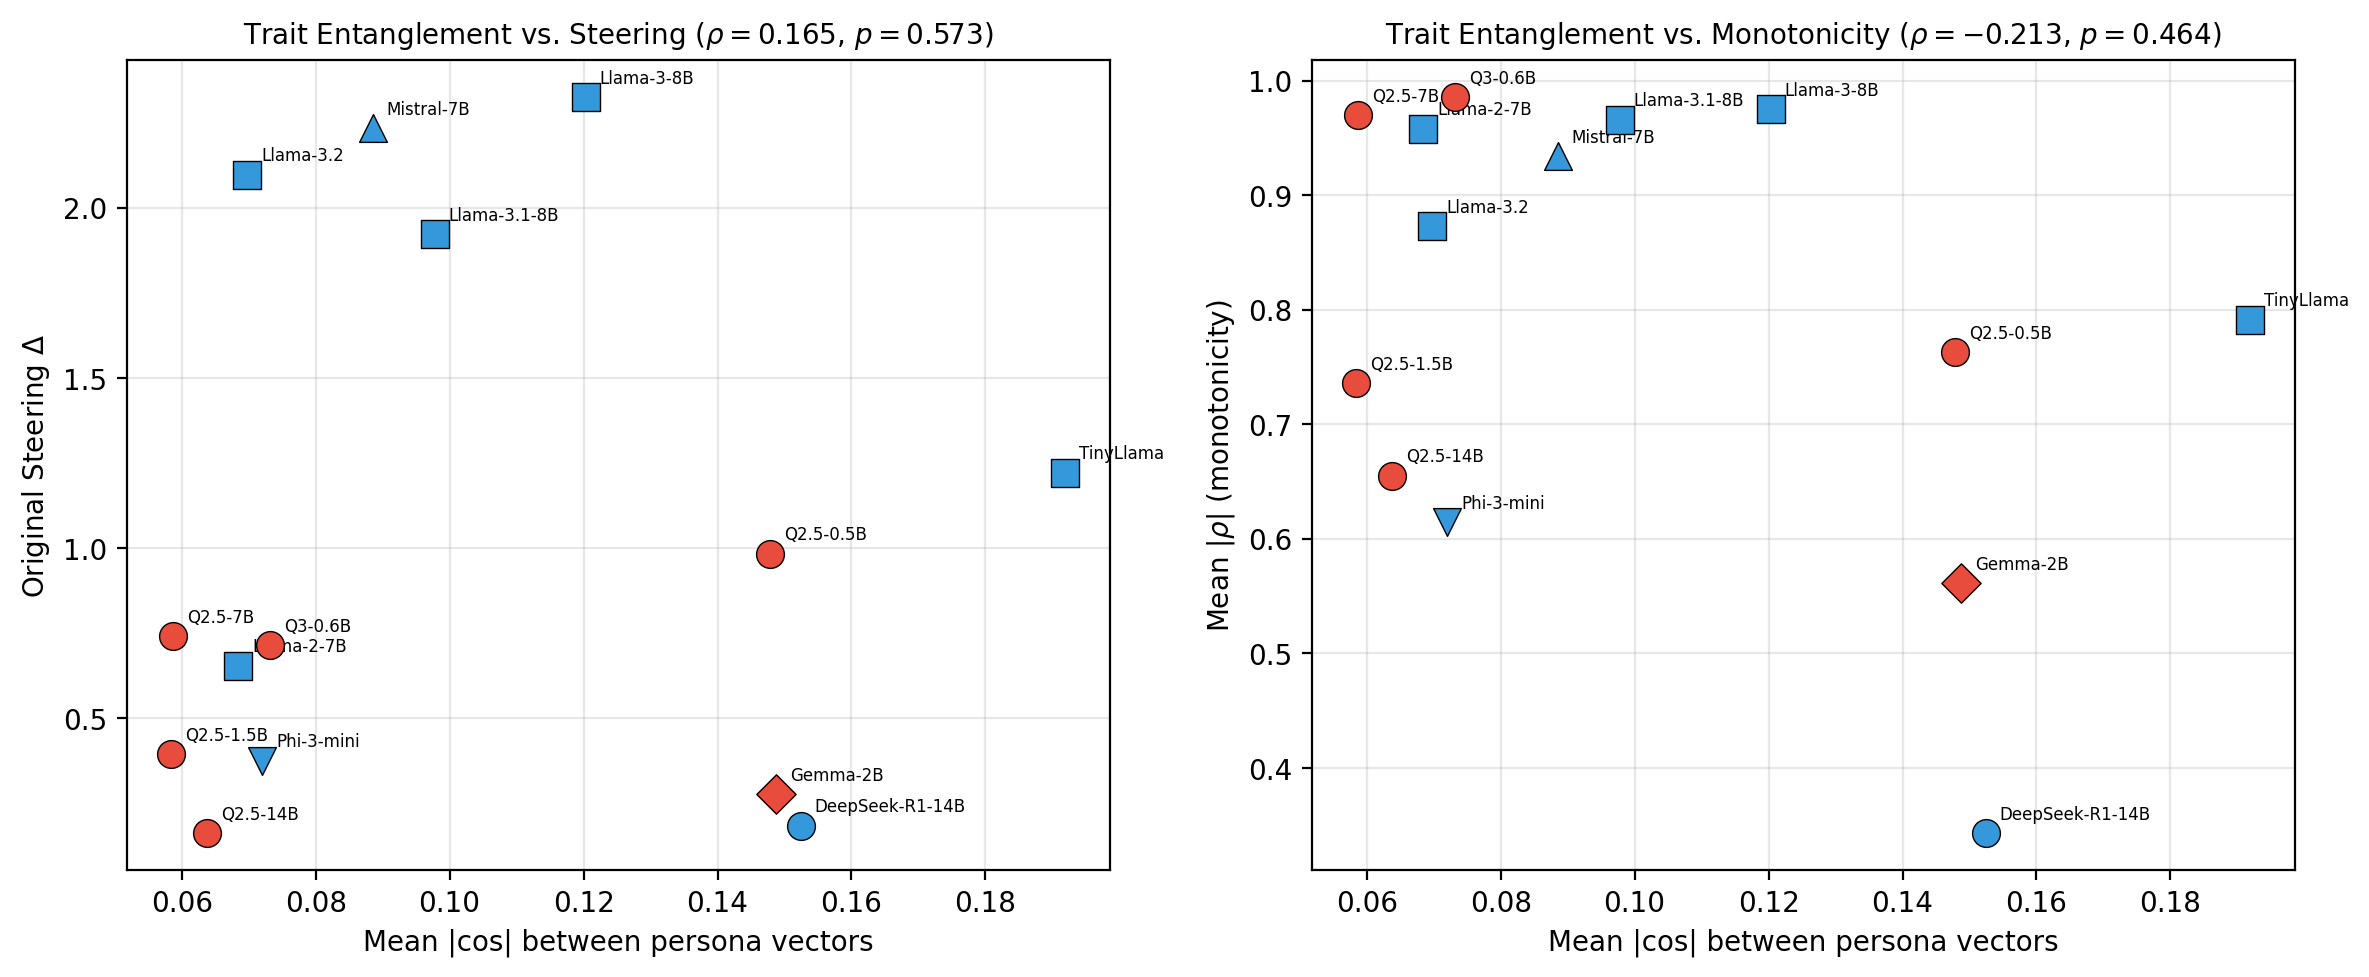
\includegraphics[width=\textwidth]{figures/fig_entanglement_analysis.png}
\caption{\textbf{Trait entanglement vs.\ steering effectiveness.} Mean $|\cos|$ between persona vectors (quantifying cross-trait correlation) plotted against steering $\Delta$. Higher entanglement does not show a clear monotonic relationship with steering, suggesting entanglement interacts with other architectural factors.}
\label{fig:entanglement}
\end{figure}

We quantify \textbf{representation entanglement} as the mean absolute cosine similarity $|\cos|$ between persona vectors at each model's best layer (Table~\ref{tab:entanglement_summary}). Values range from 0.058 (Q2.5-1.5B) to 0.192 (TinyLlama). Critically, entanglement does \emph{not} linearly predict steering effectiveness: Q2.5-1.5B has the lowest entanglement (0.058) yet remains poorly steerable, while TinyLlama has the highest (0.192) and achieves moderate steering ($\Delta$=1.22). This confirms that entanglement alone cannot explain the steering landscape---it is the \emph{interaction} between perturbation ratio, entanglement, and potentially other architectural factors (e.g., attention head distribution, layer normalization) that determines steerability.

\section{Architectural Determinants of Hidden State Scale}\label{app:architecture}

\begin{table}[h]
\caption{\textbf{Architectural parameters and hidden state scale.} RMS magnitude at the steering layer for each model, with architectural family and key hyperparameters.}
\label{tab:architecture_regression}
\centering
\small
\begin{tabular}{lcccc}
\toprule
\textbf{Model} & \textbf{Family} & \textbf{$\epsilon$} & \textbf{softcap} & \textbf{RMS} \\
\midrule
Q2.5-0.5B & Qwen2.5 & $10^{-6}$ & 0 & 0.461 \\
Q3-0.6B & Qwen3 & $10^{-6}$ & 0 & 0.333 \\
TinyLlama & LLaMA & $10^{-5}$ & 0 & 0.408 \\
Llama-3.2 & LLaMA & $10^{-5}$ & 0 & 0.094 \\
Q2.5-1.5B & Qwen2.5 & $10^{-6}$ & 0 & 0.432 \\
Gemma-2B & Gemma-2 & $10^{-6}$ & 50 & 2.500 \\
Q2.5-7B & Qwen2.5 & $10^{-6}$ & 0 & 0.308 \\
Mistral-7B & Mistral & $10^{-5}$ & 0 & 0.036 \\
Llama-3-8B$^\dagger$ & LLaMA & $10^{-5}$ & 0 & 0.123 \\
Llama-3.1-8B & LLaMA & $10^{-5}$ & 0 & 0.140 \\
\bottomrule
\multicolumn{5}{l}{\footnotesize $^\dagger$PERSONA's exact model.}
\end{tabular}
\end{table}

\begin{figure}[h]
\centering
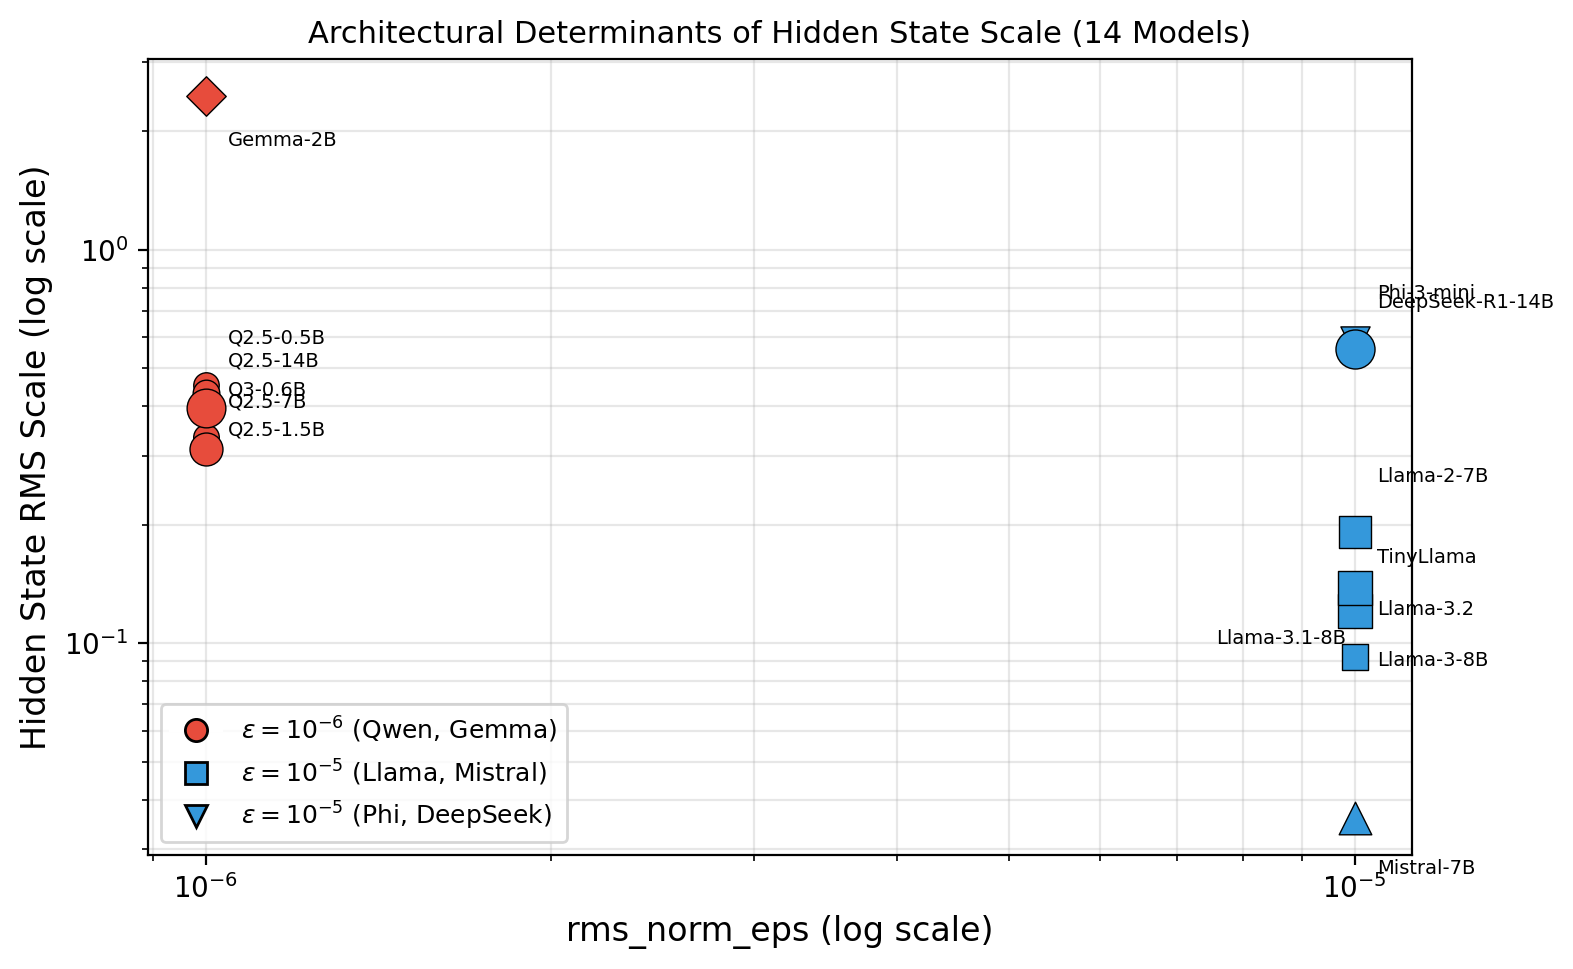
\includegraphics[width=0.85\textwidth]{figures/fig_architecture_rms.png}
\caption{\textbf{Architectural prediction of hidden state scale.} Observed vs.~predicted $\log_{10}(\text{RMS})$ from the regression $\log_{10}(\text{RMS}) \approx -0.702 \log_{10}(\epsilon) + 0.016 \cdot \text{softcap}$. Two architectural hyperparameters explain 91\% of cross-model variance in hidden state magnitude.}
\label{fig:architecture_rms}
\end{figure}

Table~\ref{tab:architecture_regression} and Figure~\ref{fig:architecture_rms} demonstrate that hidden state scale is not arbitrary but systematically determined by architecture. The layer normalization epsilon dominates: models with $\epsilon = 10^{-6}$ (Qwen, Gemma) show RMS $0.3$--$2.5$, while models with $\epsilon = 10^{-5}$ (LLaMA, Mistral) show RMS $0.04$--$0.13$---a $10\times$ difference driven by a single hyperparameter. Attention softcapping (Gemma-2B: softcap=50) contributes an additional multiplicative effect.

\section{Method Details}\label{app:method_details}

\subsection{Metrics and Evaluation Criteria}

We evaluate personality encoding through four complementary metrics.

\paragraph{Leave-One-Scenario-Out (LOSO) Accuracy.}
Given $K$ contrastive pairs per trait, we train a linear probe on $K{-}1$ pairs and evaluate on the held-out pair. Repeating over all $K$ folds yields LOSO accuracy $a_\ell \in [0,1]$, measuring generalization to unseen contexts.

\paragraph{Cohen's $d$ Effect Size.}
At layer $\ell$, we compute standardized mean separation between high-trait and low-trait activations:
\begin{equation}
d_\ell = \frac{\mu_{+,\ell} - \mu_{-,\ell}}{\sqrt{\frac{(n_+-1)s_{+,\ell}^2 + (n_--1)s_{-,\ell}^2}{n_+ + n_- - 2}}}
\end{equation}
Values $d > 0.8$ indicate large effects; our models consistently achieve $d > 2.0$.

\paragraph{Signal-to-Noise Ratio (SNR).}
To distinguish genuine signal from scaling artifacts:
\begin{equation}
\text{SNR}_\ell = \frac{\|v^{\text{diff}}_\ell\| / \text{RMS}_\ell}{\mathbb{E}[\|v^{\text{random}}_\ell\| / \text{RMS}_\ell]}
\end{equation}
SNR $> 2$ indicates contrastive signal exceeds random noise; our models achieve SNR $> 7$.

\paragraph{Perturbation Ratio (PR).}
Defined as PR = $\alpha / \|h\|$, this metric normalizes intervention strength by hidden state magnitude for cross-model comparability.

\subsection{Extraction Method Convergence}

Mean-difference vectors show mean $|\cos| > 0.95$ with PCA first components and $|\cos| > 0.89$ with linear probe weights across all traits and models. This high collinearity indicates personality directions are robustly identifiable despite theoretical non-identifiability concerns.

\subsection{Statistical Power and Sample Size}

With $K=20$ scenario pairs per Big Five trait, bootstrap standard errors are $<0.02$ for accuracy and $<0.15$ for Cohen's $d$. For defense mechanisms ($K=10$), accuracy standard errors remain $<0.03$, sufficient given larger effect sizes ($d > 2.0$).

\subsection{Sample Size Ablation}

Comparing random ($n=5$) vs.\ Cartesian product ($n=160$) designs on Qwen3 Openness shows a 2.44$\times$ increase in effect size (from $d=2.69$ to $d=6.57$), establishing that prior work using $n=5$--$20$ systematically underestimates signal strength.

% ============================================================
\section{Per-Model Detailed Results}\label{app:permodel}

This appendix presents the full per-model experimental results, including layer-wise encoding profiles, orthogonality matrices, causal localization maps, and steering curves for each individual model.

\subsection{Qwen2.5-0.5B-Instruct}

\begin{figure}[H]
\centering
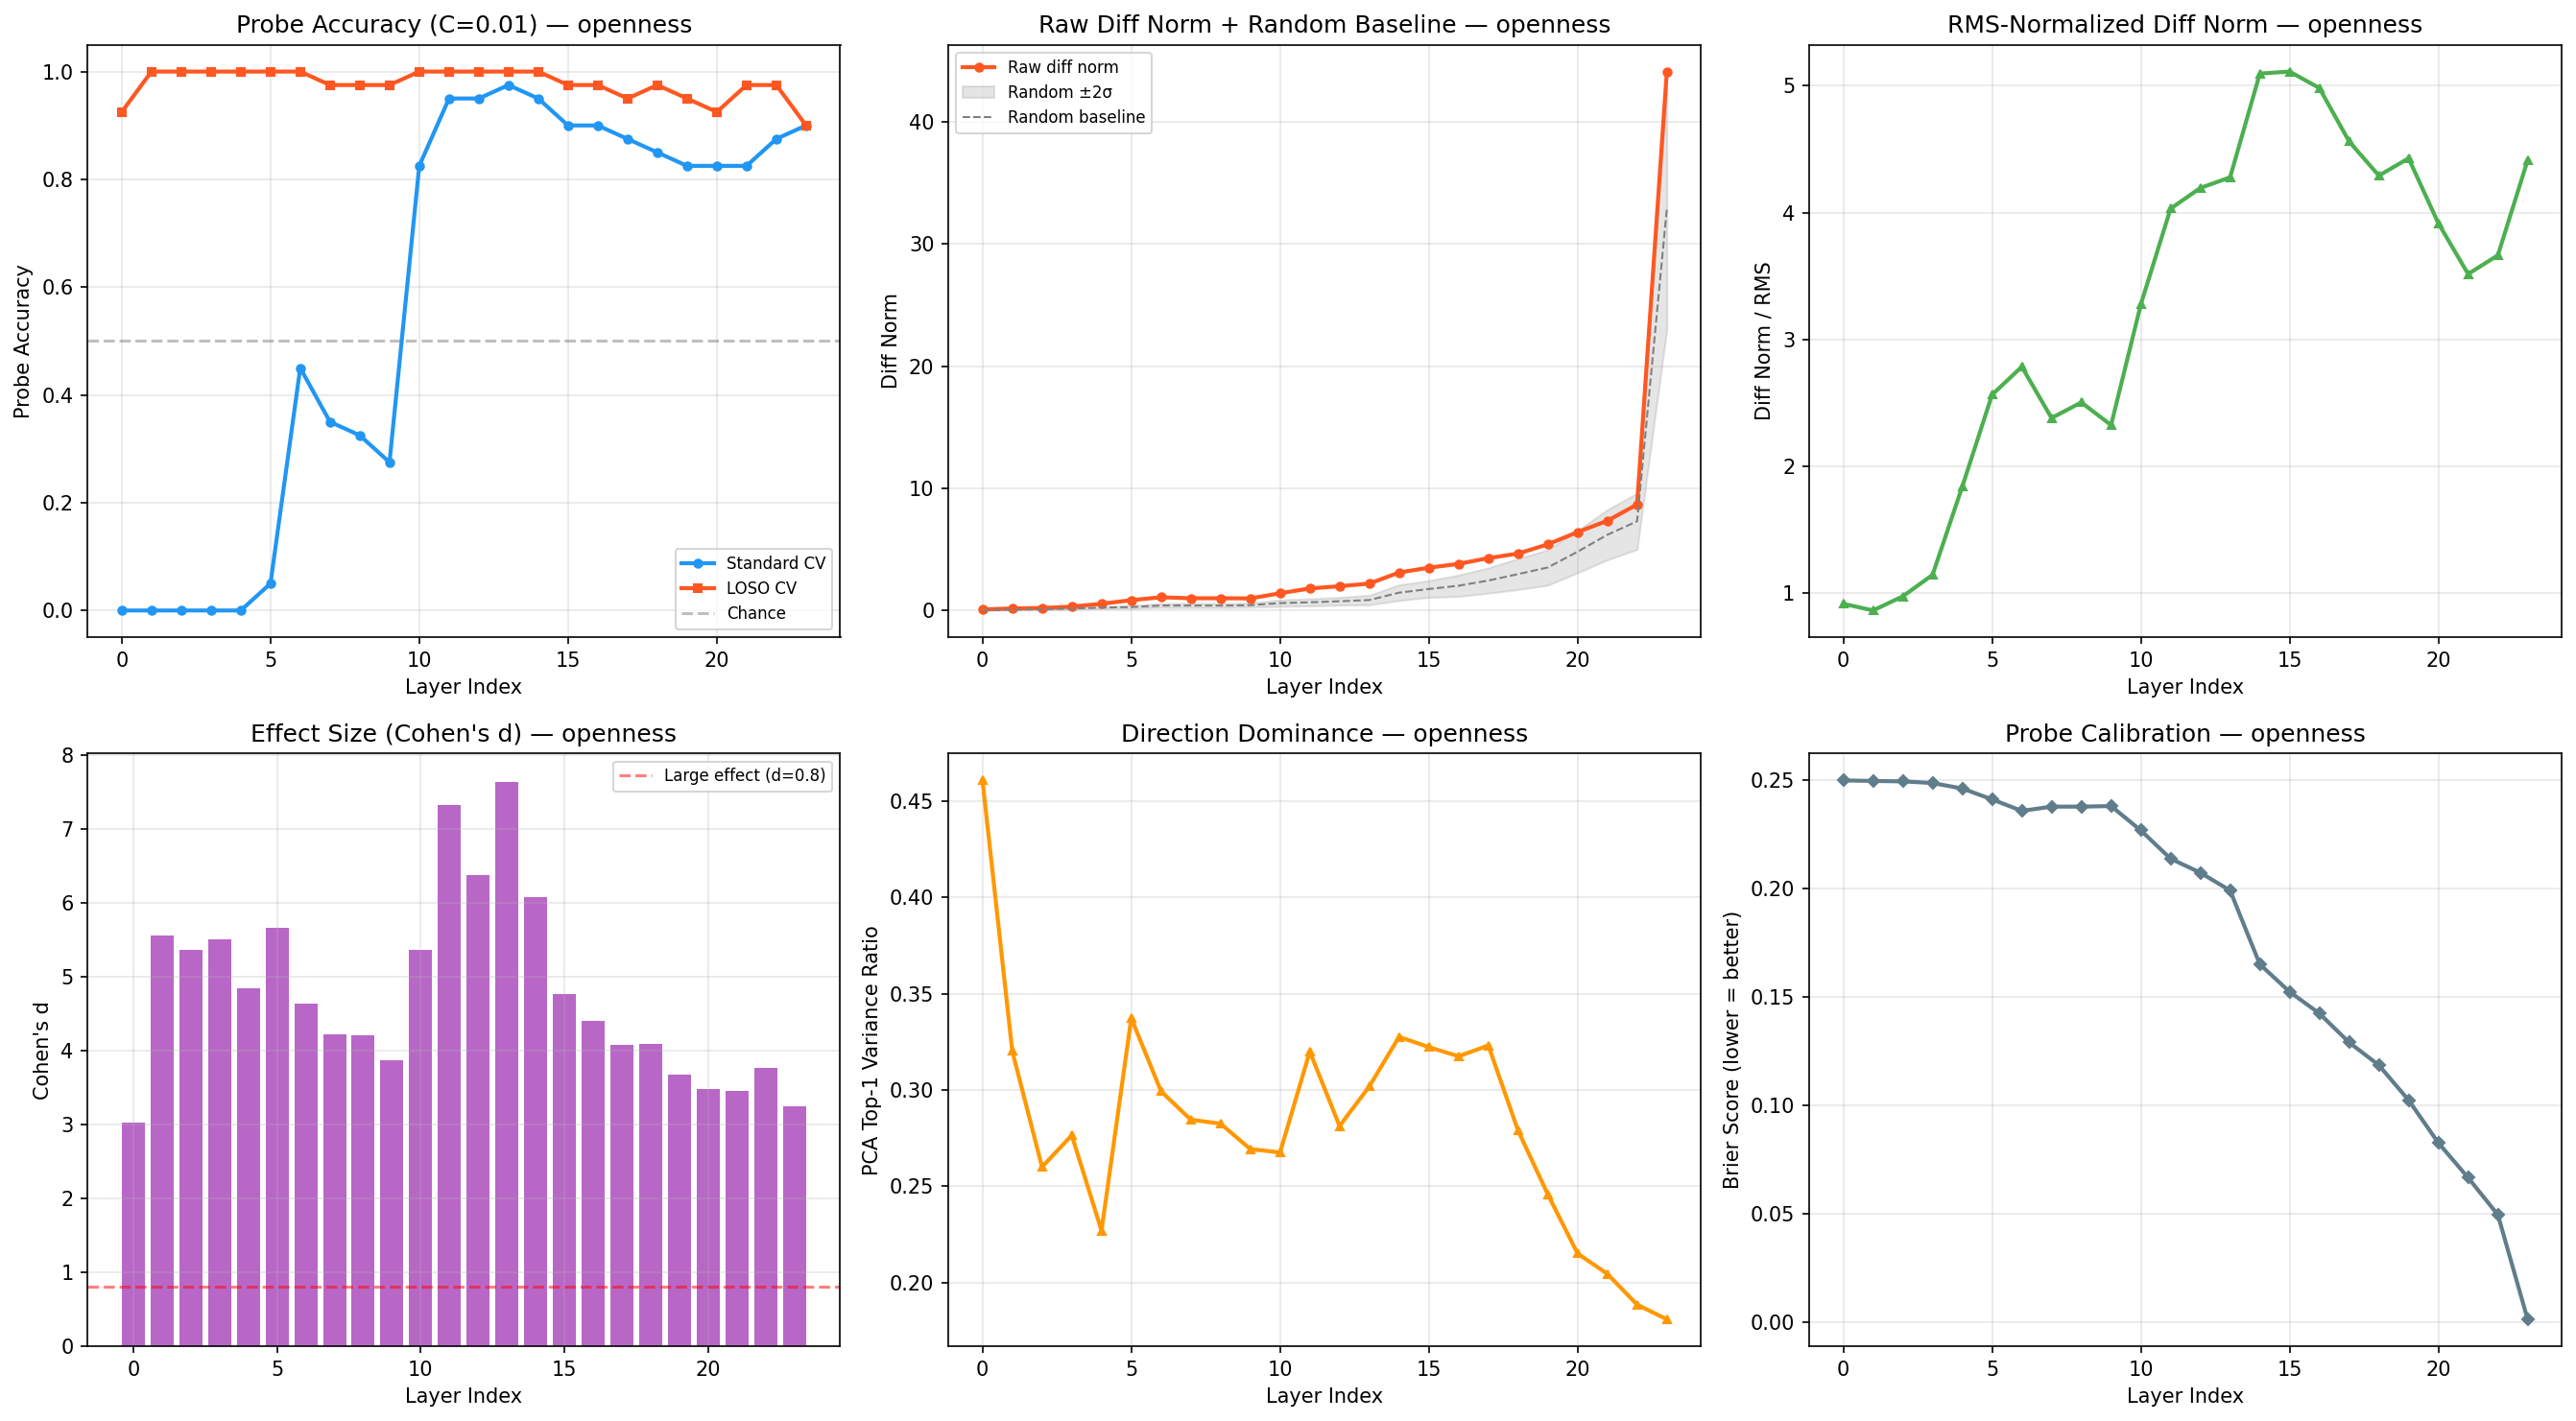
\includegraphics[width=\textwidth]{figures/layer_profile_Qwen_Qwen2.5-0.5B-Instruct_openness.png}
\caption{\textbf{Qwen2.5-0.5B-Instruct: Layer-wise personality encoding profile for Openness.}
Linear probe accuracy, Mean difference norm, and PCA explained variance.}
\label{fig:Qwen_Qwen2.5-0.5B-Instruct_layer}
\end{figure}

\begin{figure}[H]
\centering
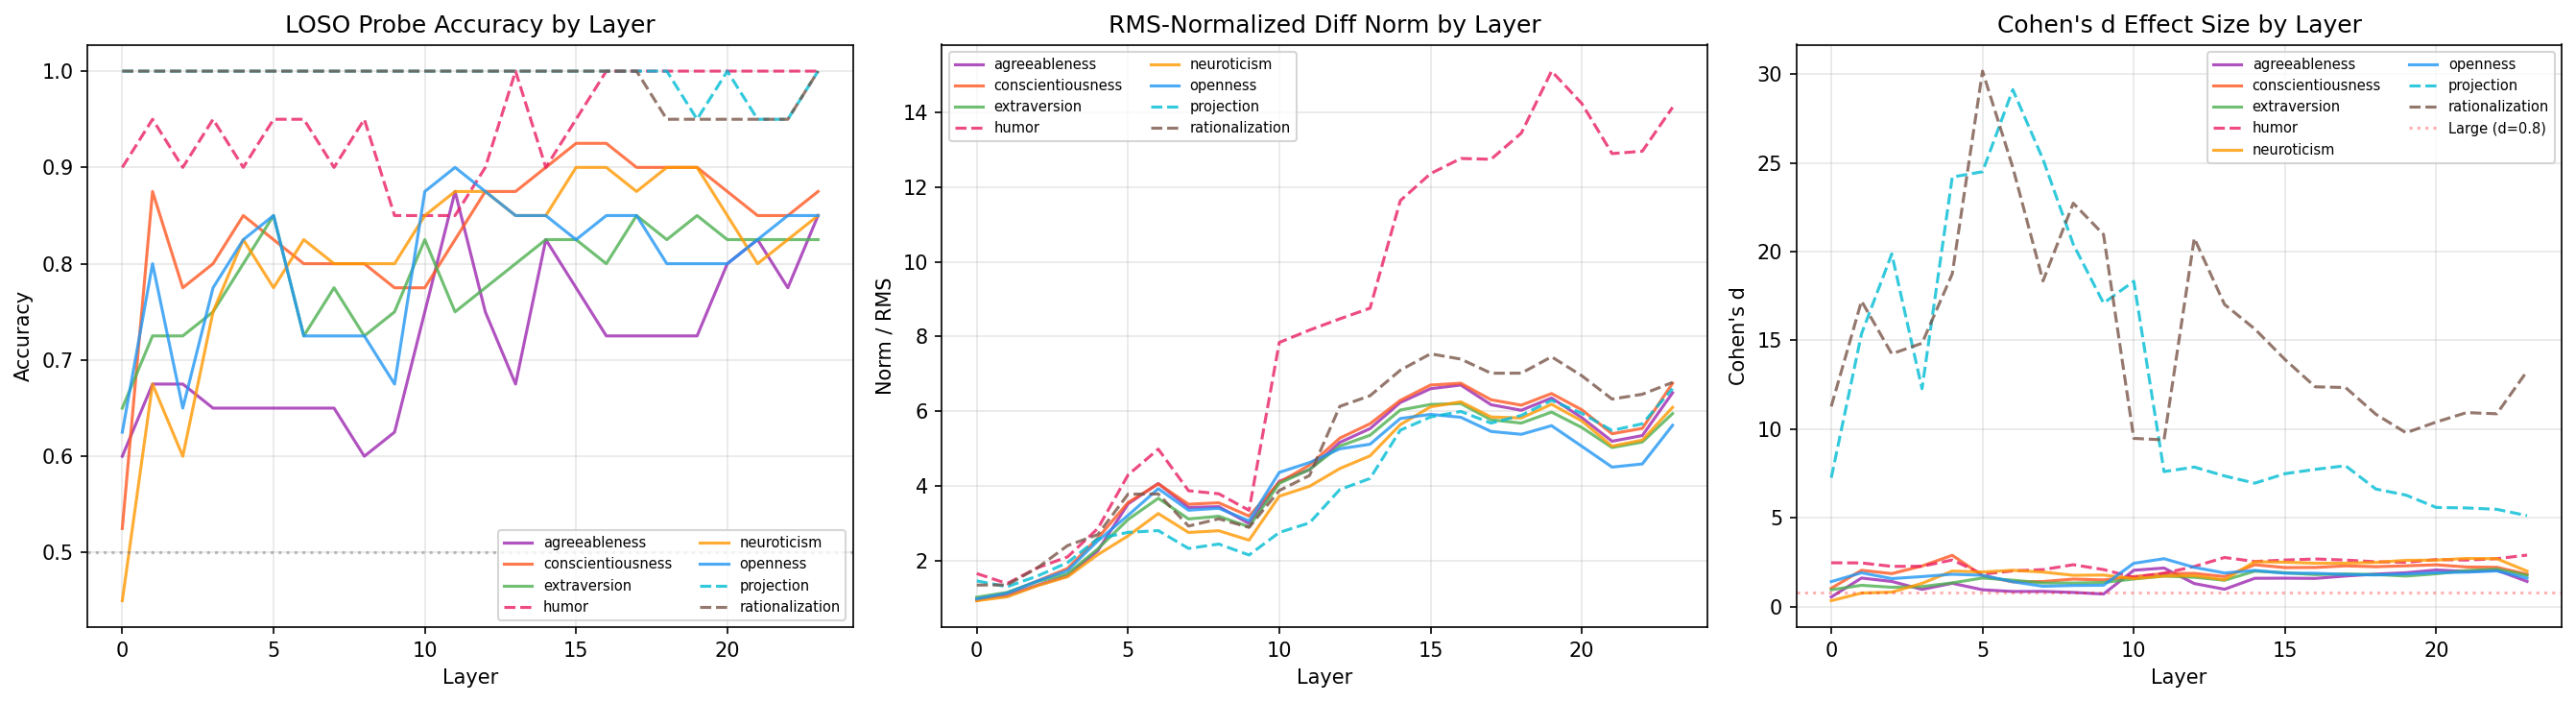
\includegraphics[width=\textwidth]{figures/ortho_Qwen_Qwen2.5-0.5B-Instruct.png}
\caption{\textbf{Qwen2.5-0.5B-Instruct: Cosine similarity matrix between persona vectors.}}
\label{fig:Qwen_Qwen2.5-0.5B-Instruct_ortho}
\end{figure}

\clearpage

\subsection{Qwen3-0.6B}

\begin{figure}[H]
\centering
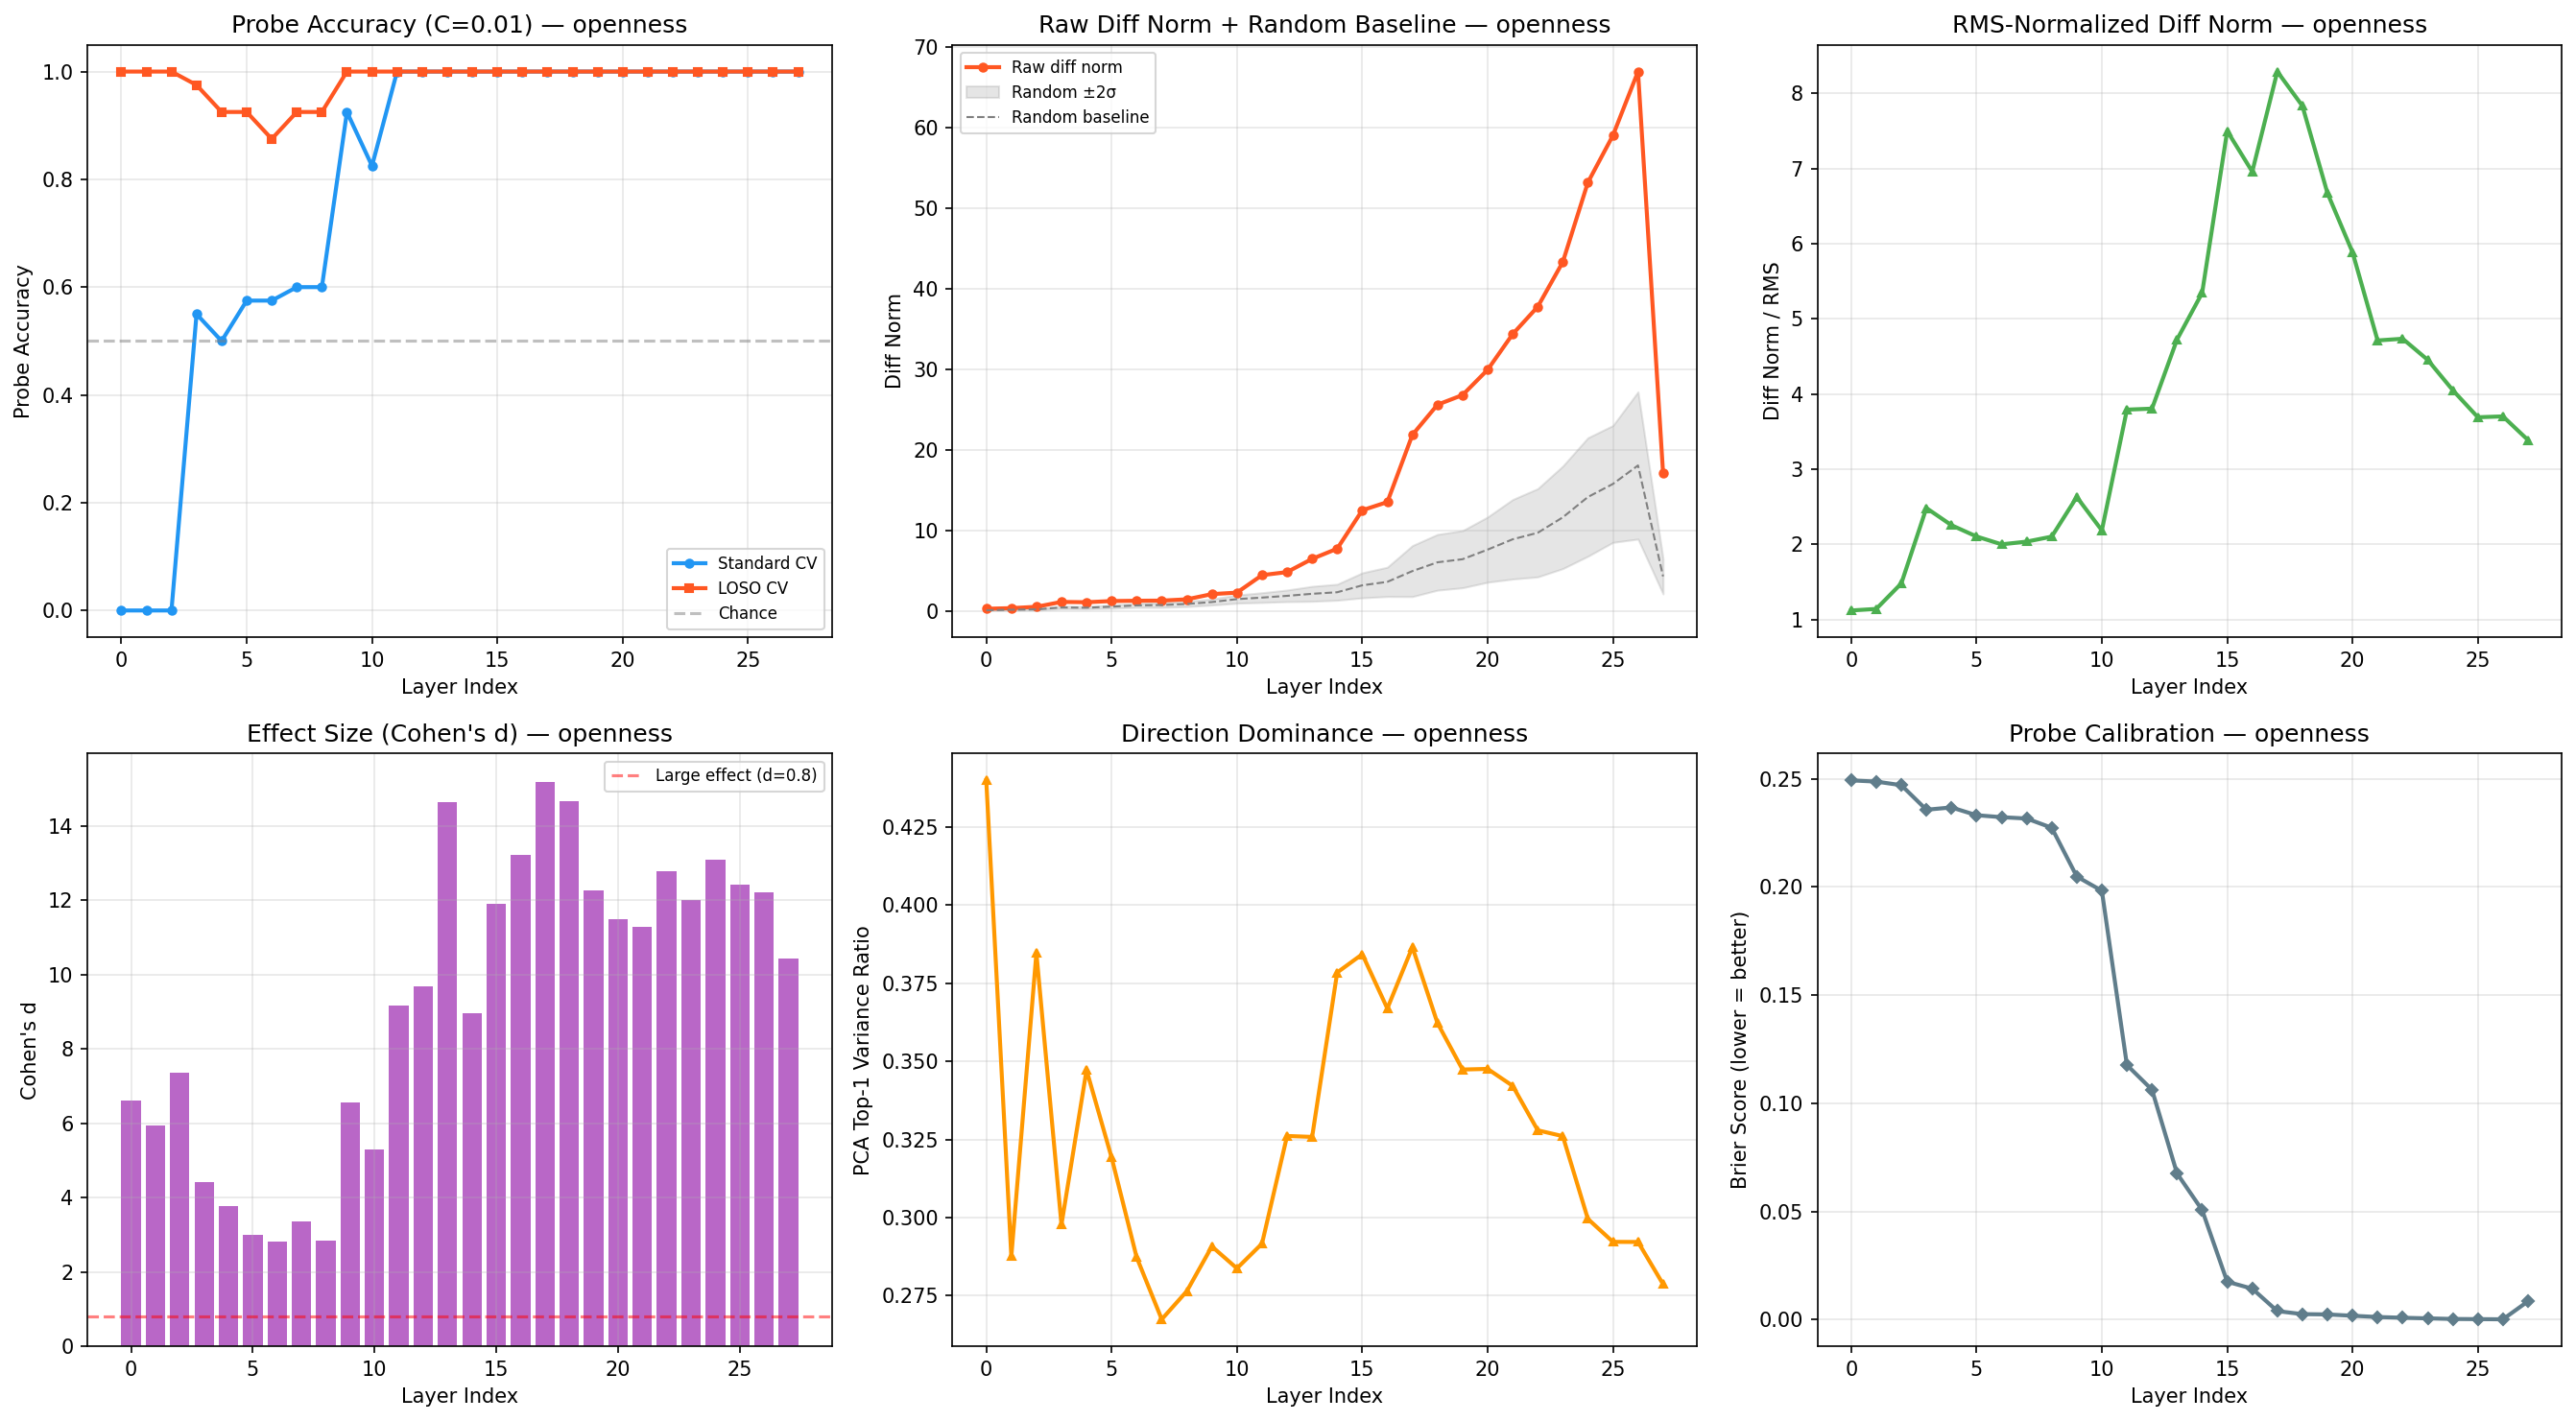
\includegraphics[width=\textwidth]{figures/layer_profile_Qwen_Qwen3-0.6B_openness.png}
\caption{\textbf{Qwen3-0.6B: Layer-wise personality encoding profile for Openness.}}
\label{fig:Qwen_Qwen3-0.6B_layer}
\end{figure}

\begin{figure}[H]
\centering
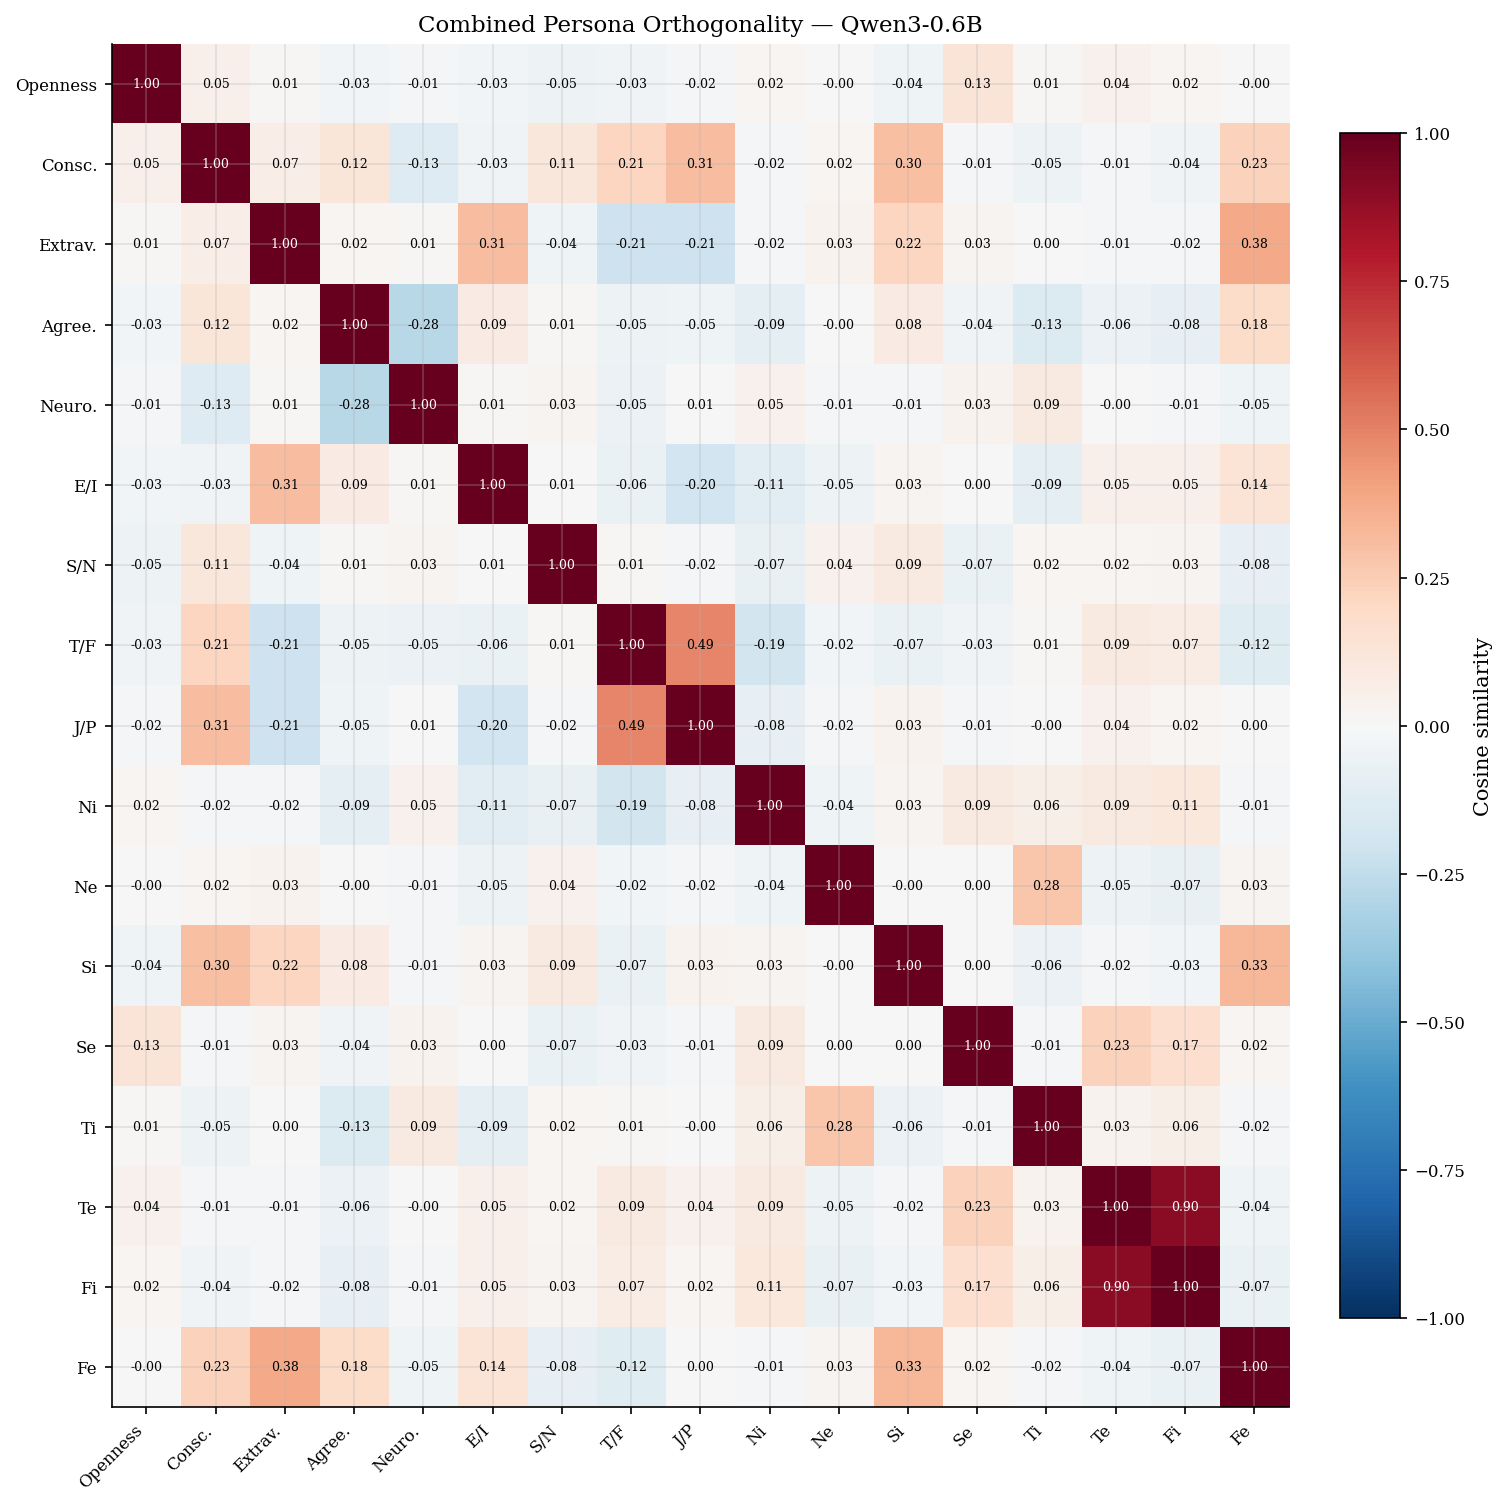
\includegraphics[width=\textwidth]{figures/ortho_Qwen_Qwen3-0.6B.png}
\caption{\textbf{Qwen3-0.6B: Cosine similarity matrix between persona vectors.}}
\label{fig:Qwen_Qwen3-0.6B_ortho}
\end{figure}

\clearpage

\subsection{TinyLlama-1.1B}

\begin{figure}[H]
\centering
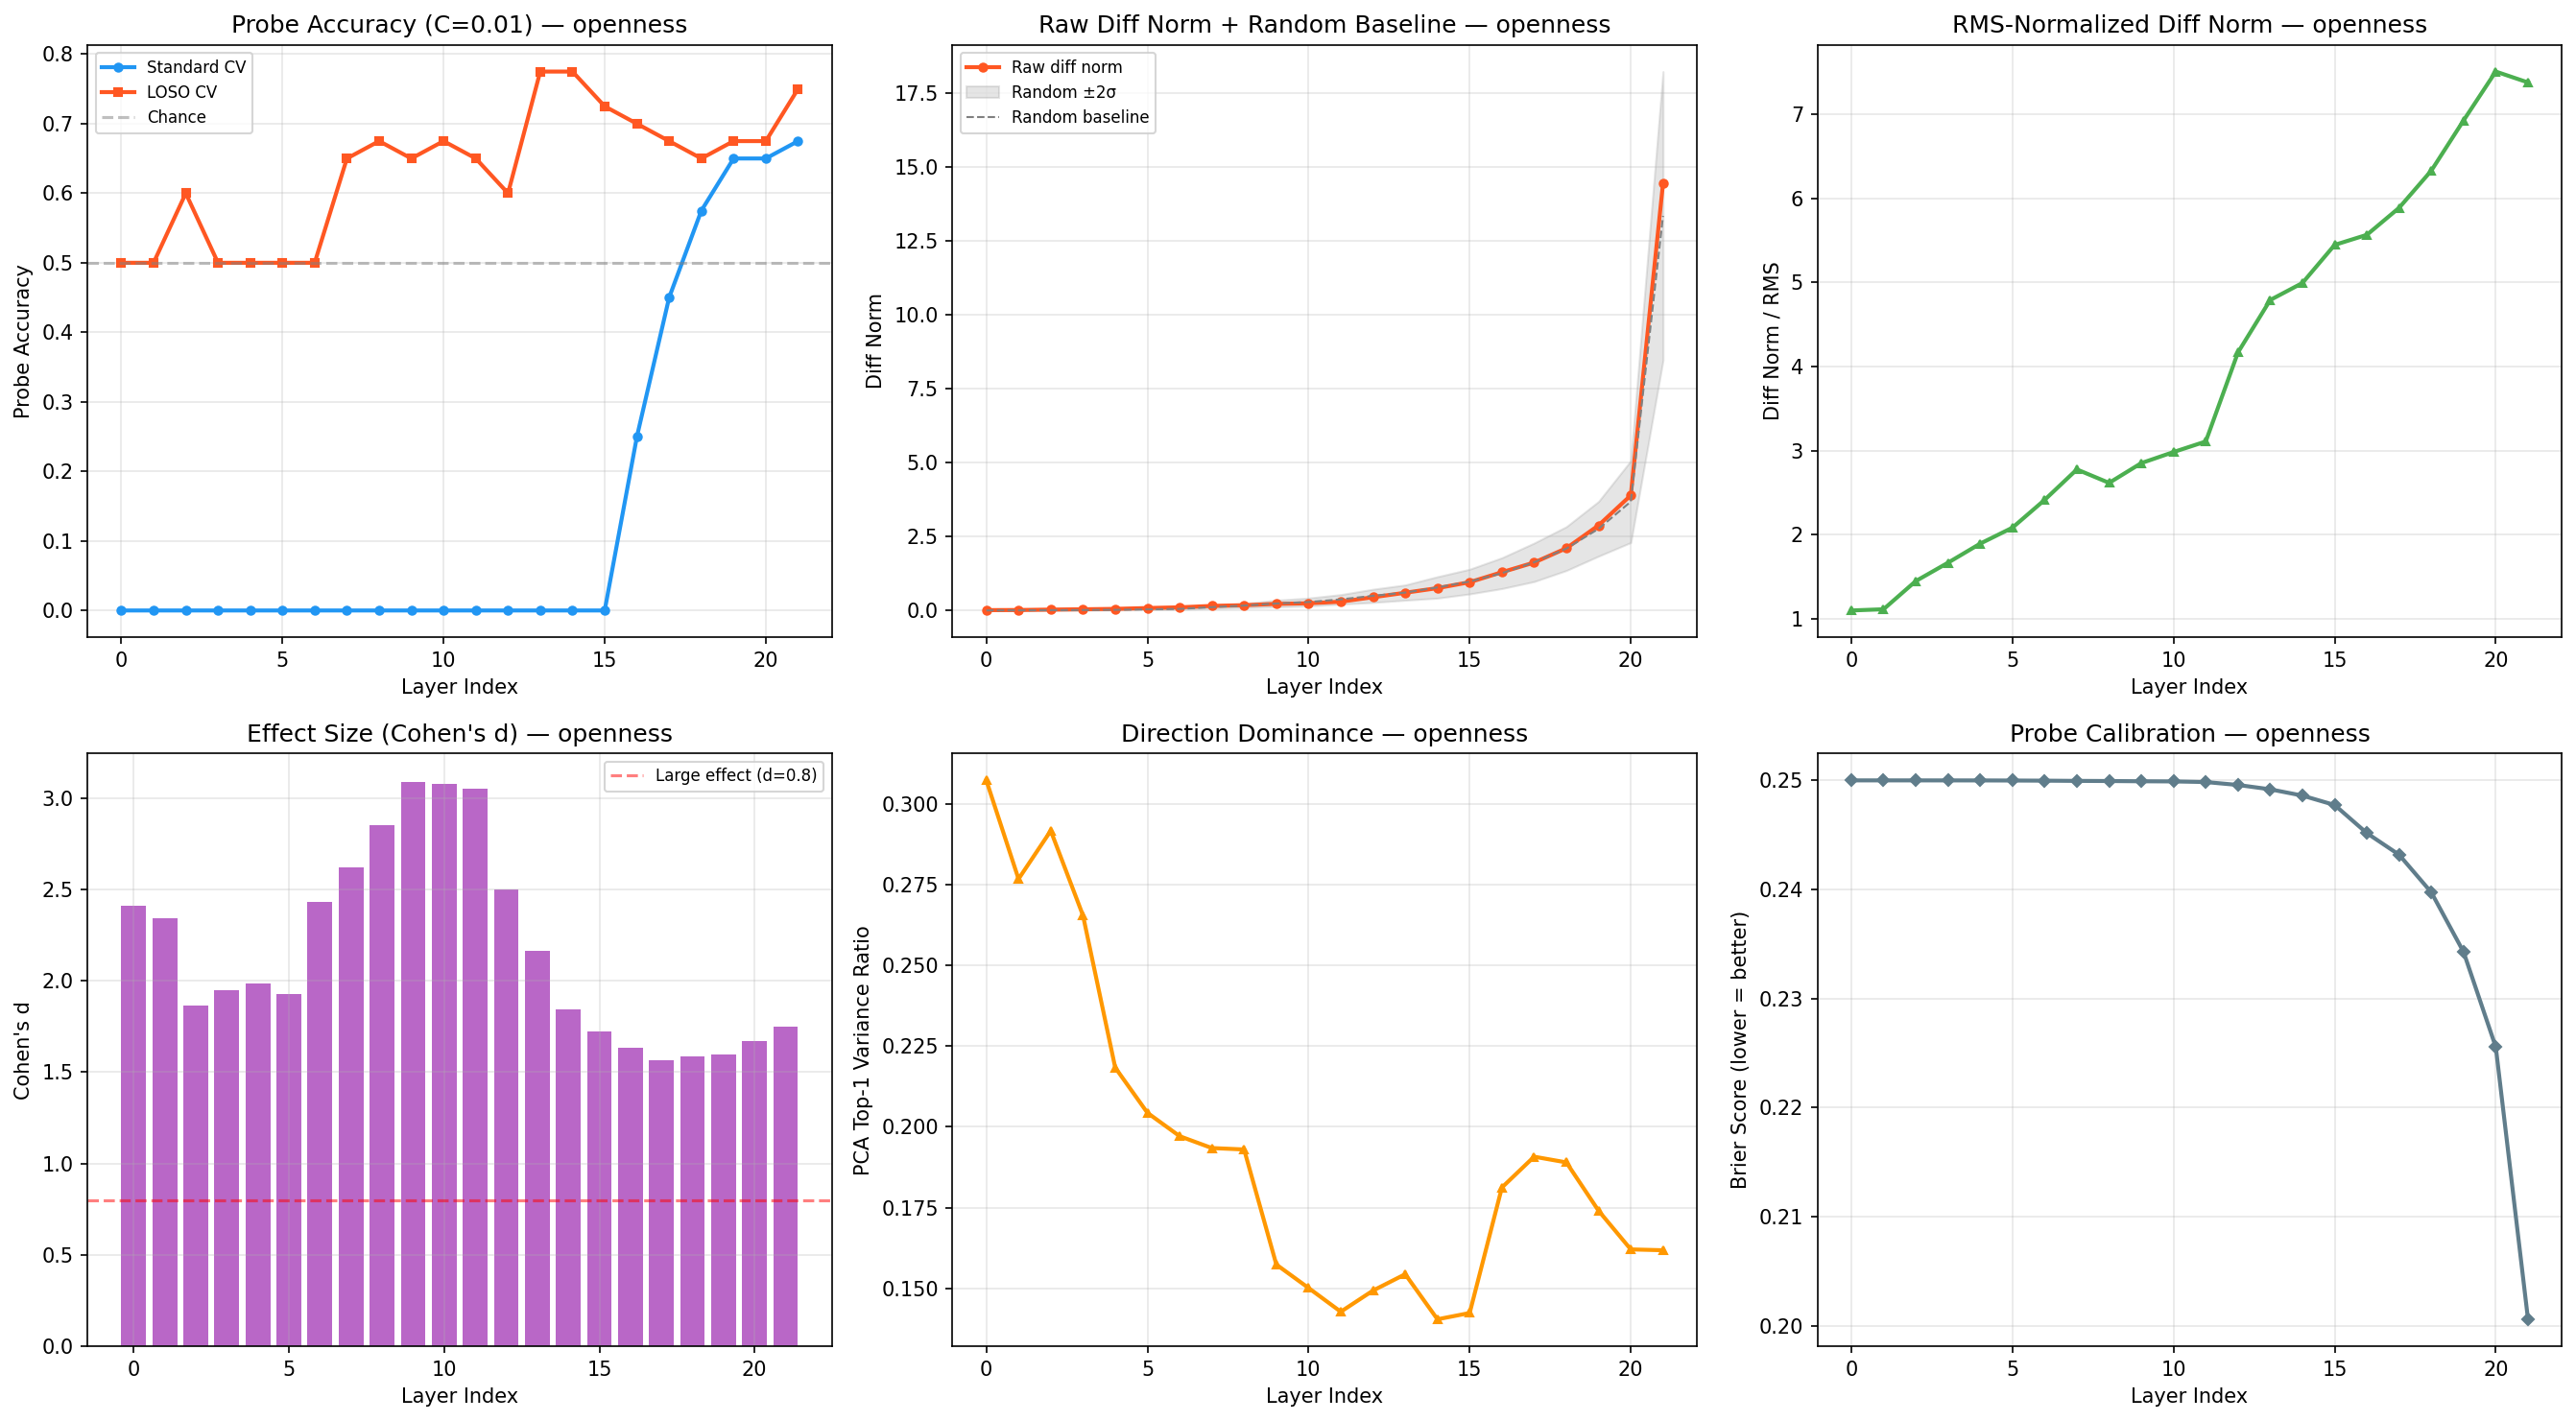
\includegraphics[width=\textwidth]{figures/layer_profile_TinyLlama_TinyLlama-1.1B-Chat-v1.0_openness.png}
\caption{\textbf{TinyLlama-1.1B: Layer-wise personality encoding profile for Openness.}}
\label{fig:TinyLlama_TinyLlama-1.1B-Chat-v1.0_layer}
\end{figure}

\begin{figure}[H]
\centering
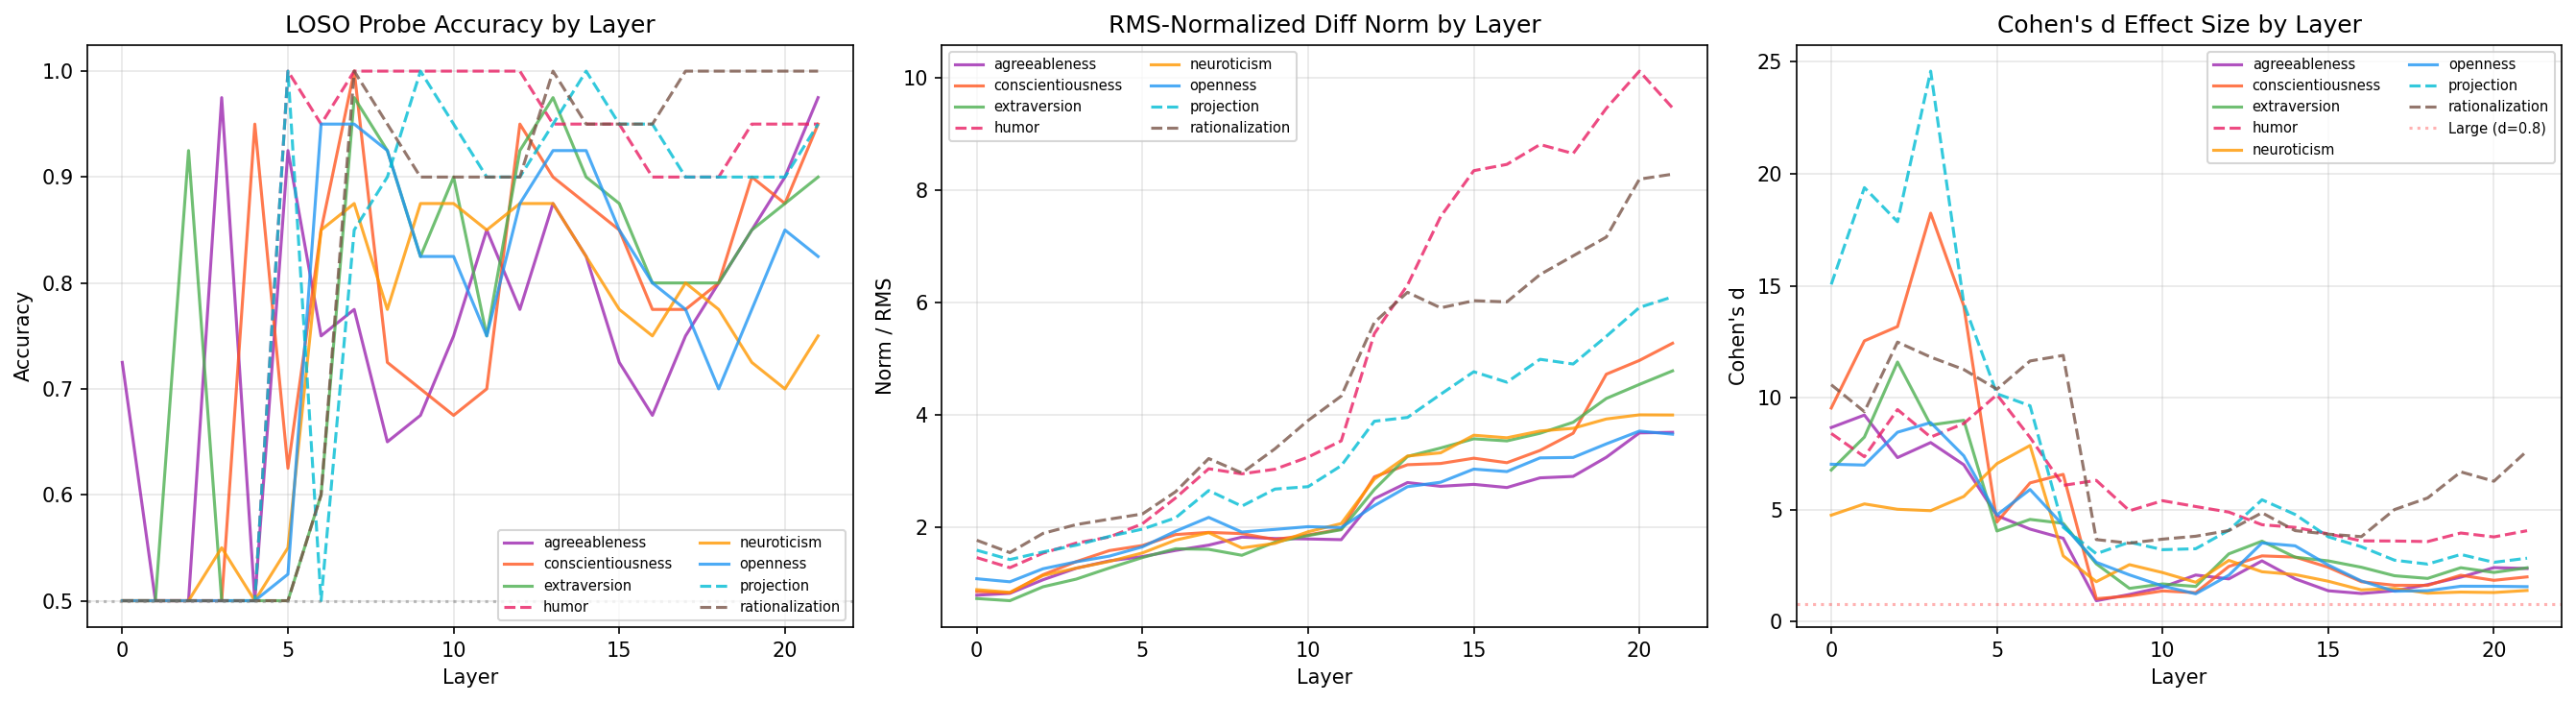
\includegraphics[width=\textwidth]{figures/ortho_TinyLlama_TinyLlama-1.1B-Chat-v1.0.png}
\caption{\textbf{TinyLlama-1.1B: Cosine similarity matrix between persona vectors.}}
\label{fig:TinyLlama_TinyLlama-1.1B-Chat-v1.0_ortho}
\end{figure}

\clearpage

\subsection{Llama-3.2-1B-Instruct}

\begin{figure}[H]
\centering
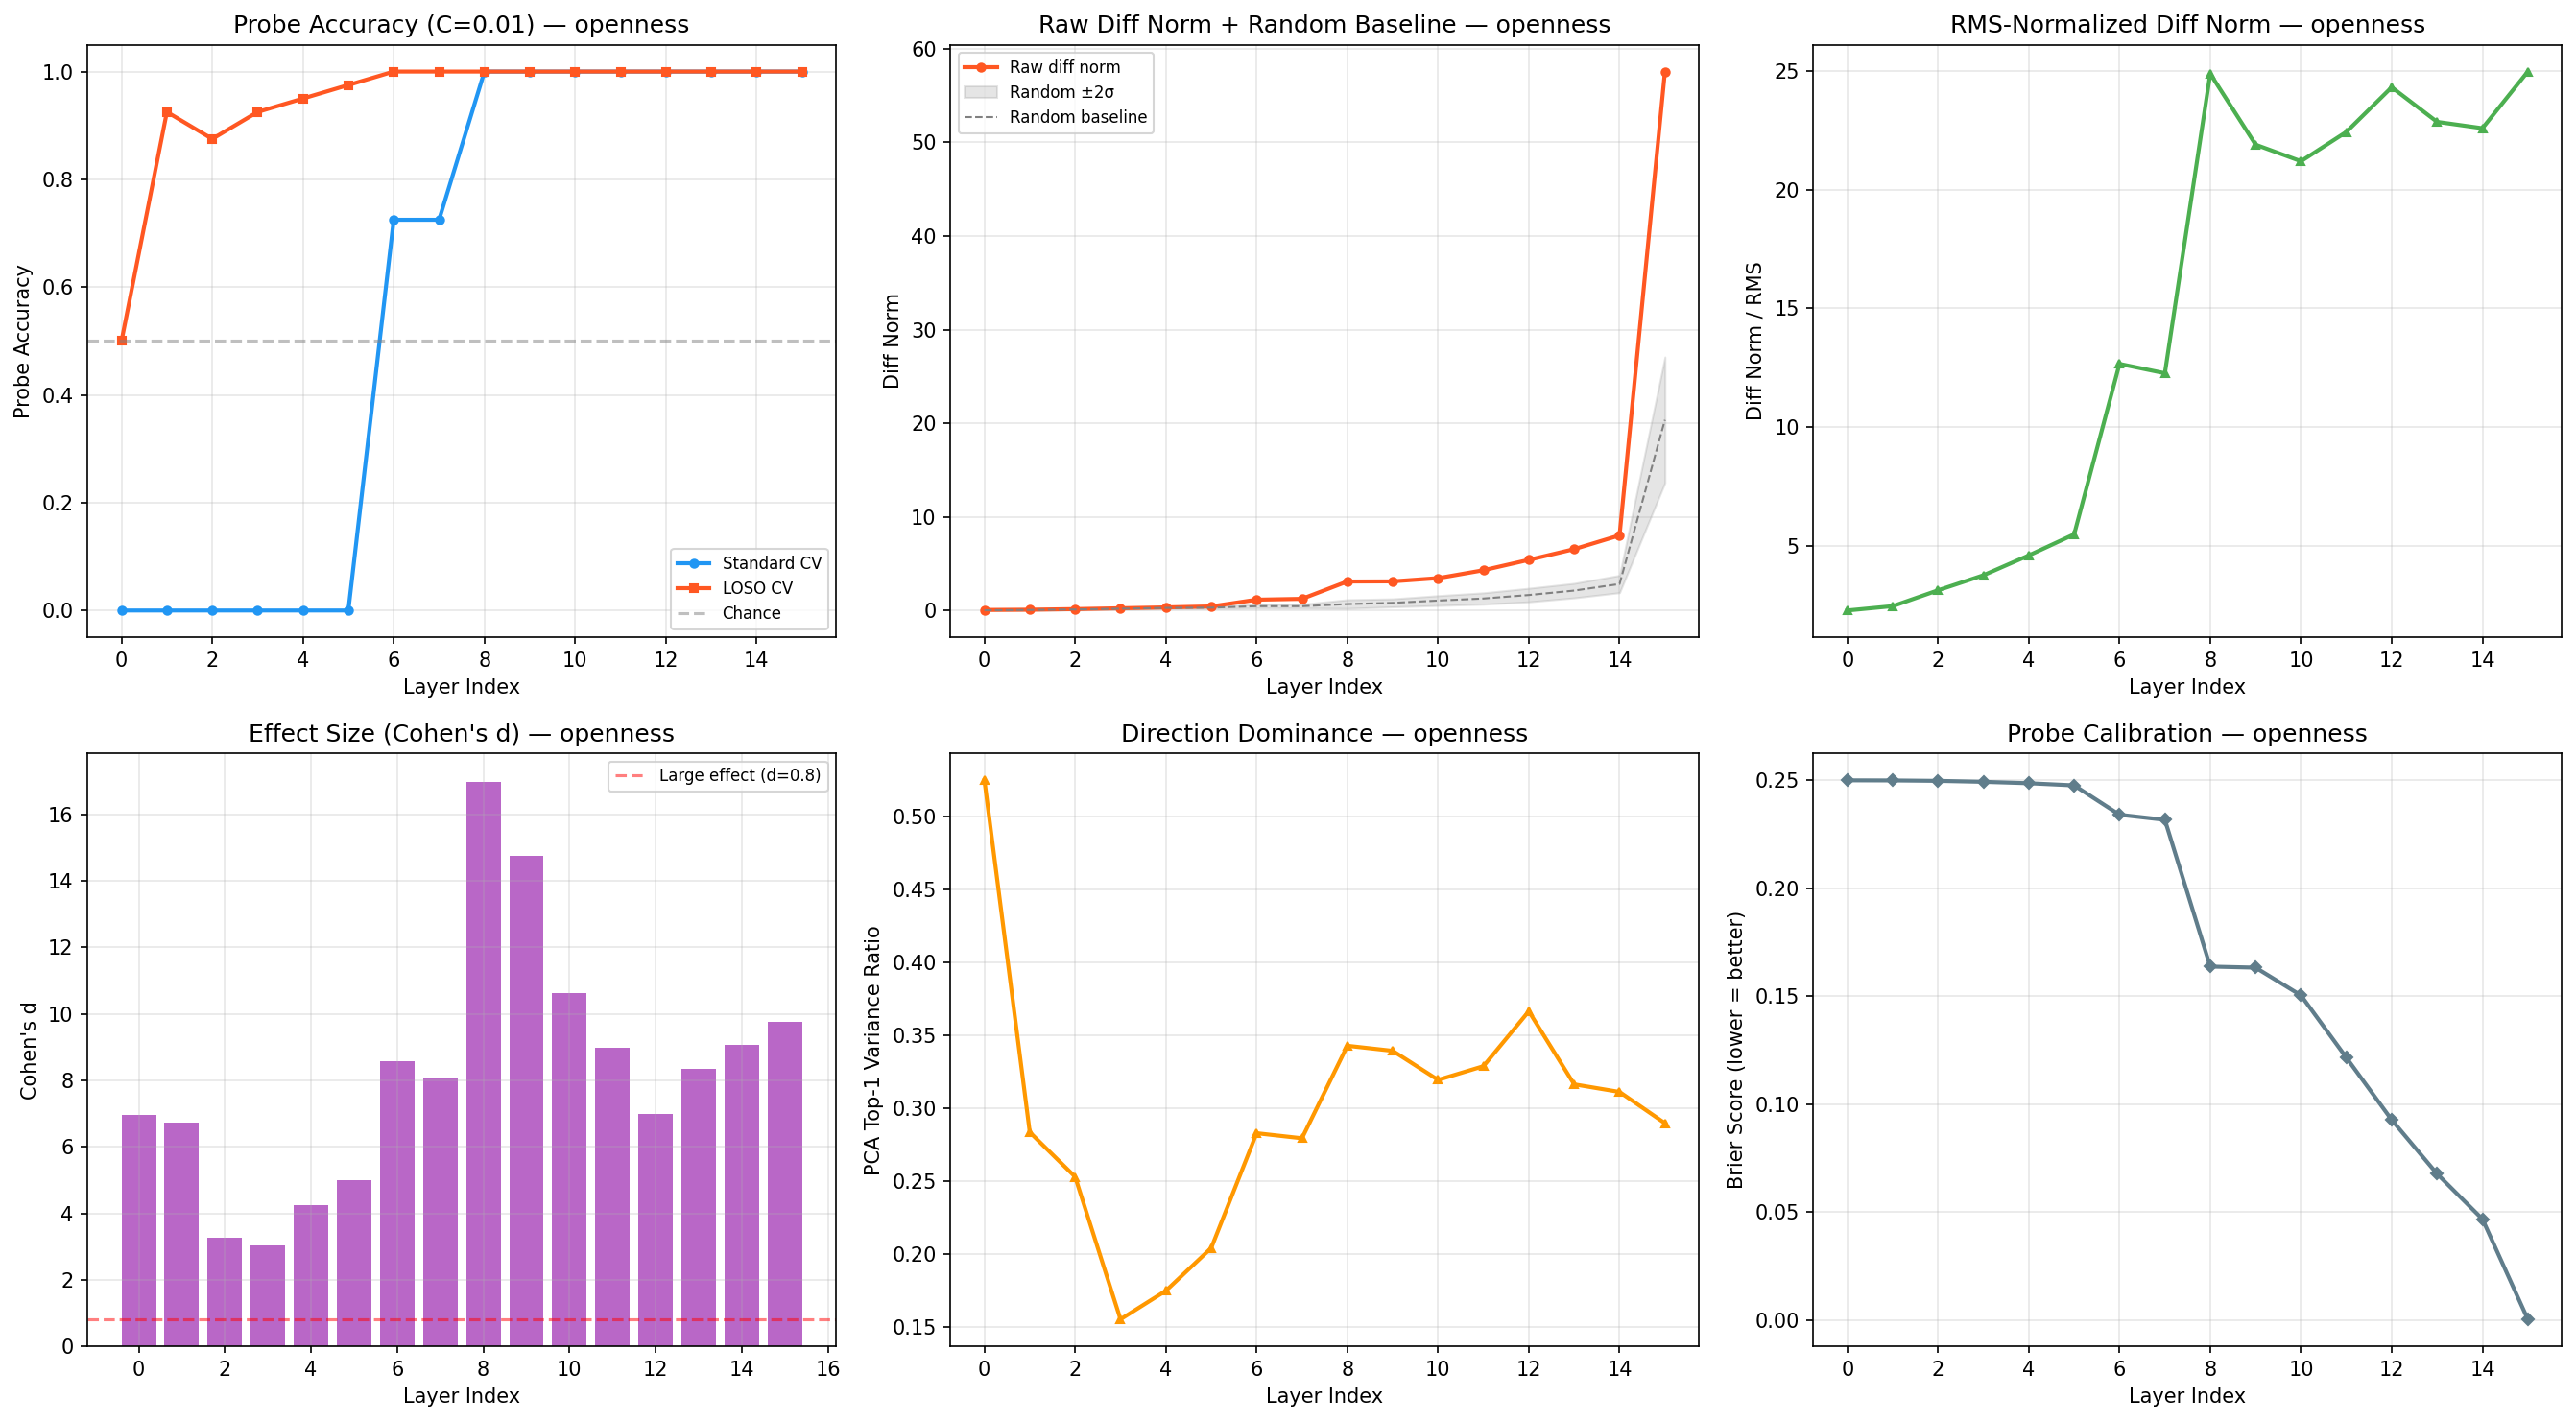
\includegraphics[width=\textwidth]{figures/layer_profile_unsloth_Llama-3.2-1B-Instruct_openness.png}
\caption{\textbf{Llama-3.2-1B-Instruct: Layer-wise personality encoding profile for Openness.}}
\label{fig:unsloth_Llama-3.2-1B-Instruct_layer}
\end{figure}

\begin{figure}[H]
\centering
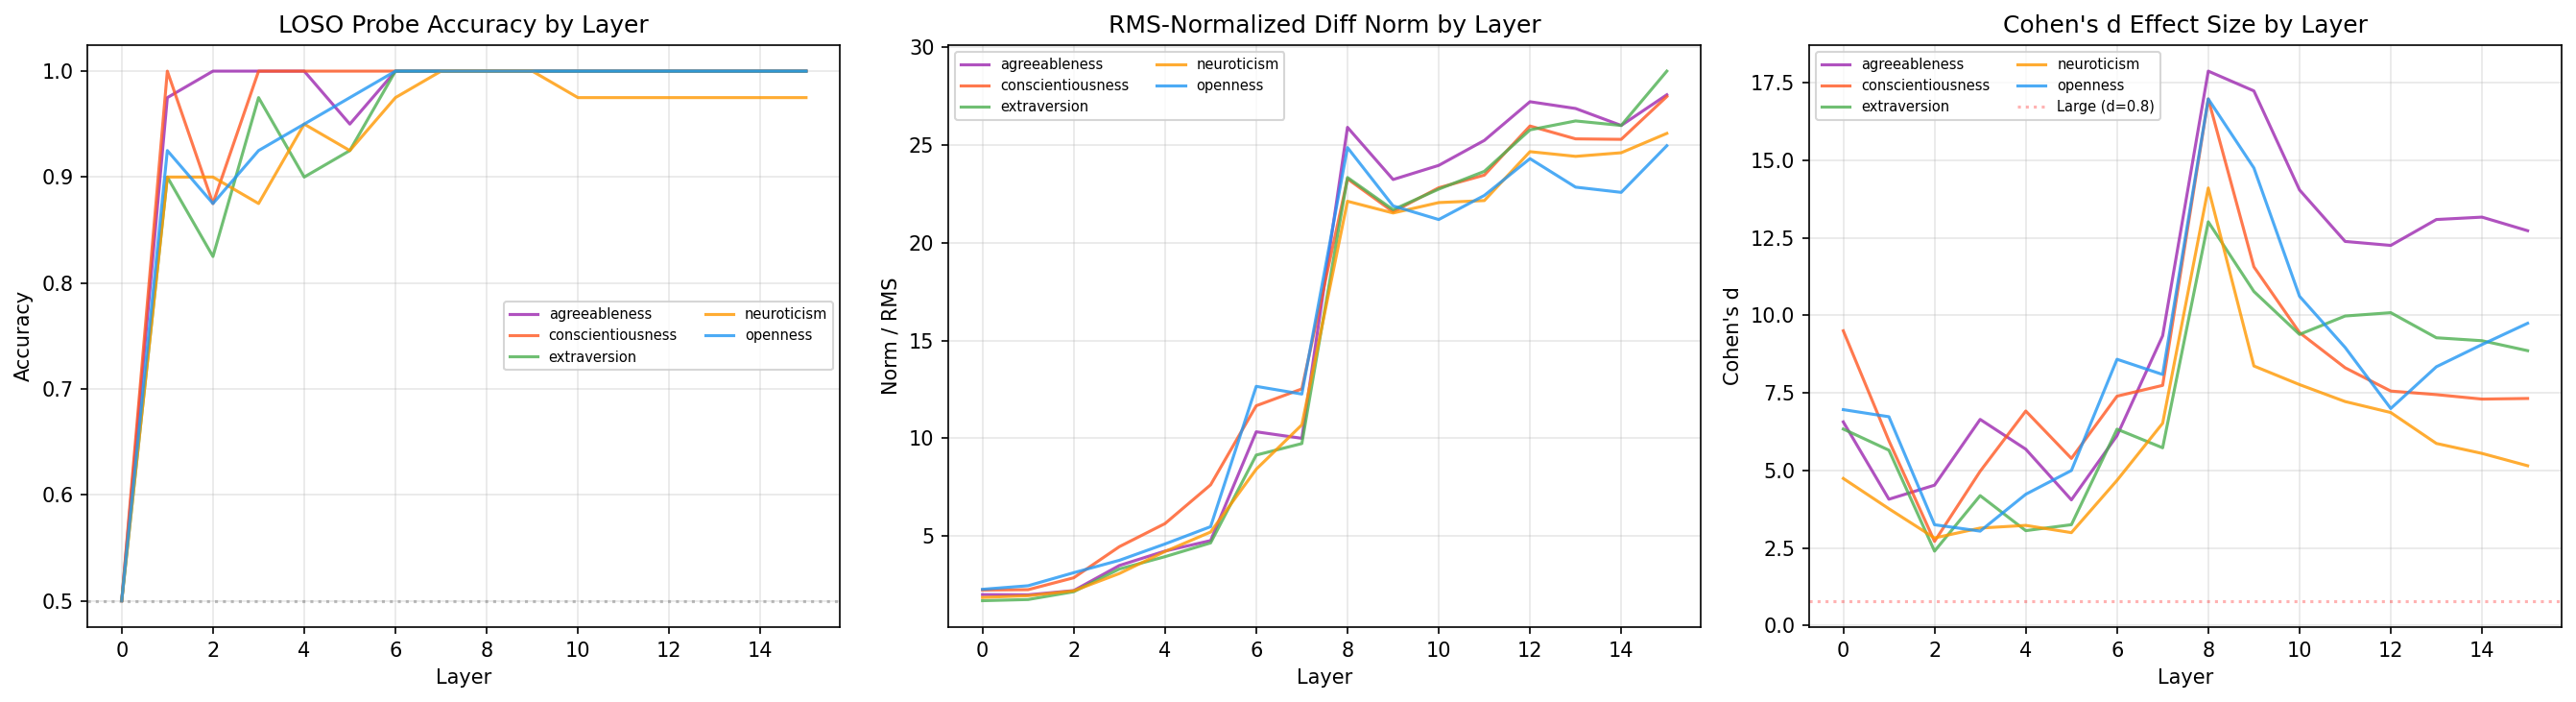
\includegraphics[width=\textwidth]{figures/ortho_unsloth_Llama-3.2-1B-Instruct.png}
\caption{\textbf{Llama-3.2-1B-Instruct: Cosine similarity matrix between persona vectors.}}
\label{fig:unsloth_Llama-3.2-1B-Instruct_ortho}
\end{figure}

\clearpage

\subsection{Gemma-2-2B-Instruct}

\begin{figure}[H]
\centering
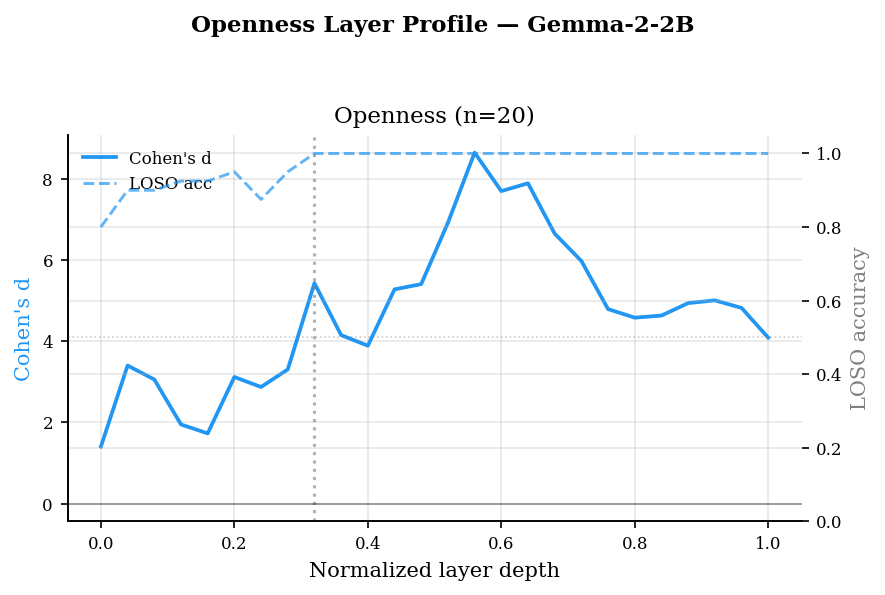
\includegraphics[width=\textwidth]{figures/layer_profile_unsloth_gemma-2-2b-it_openness.png}
\caption{\textbf{Gemma-2-2B-Instruct: Layer-wise personality encoding profile for Openness.}}
\label{fig:unsloth_gemma-2-2b-it_layer}
\end{figure}

\begin{figure}[H]
\centering
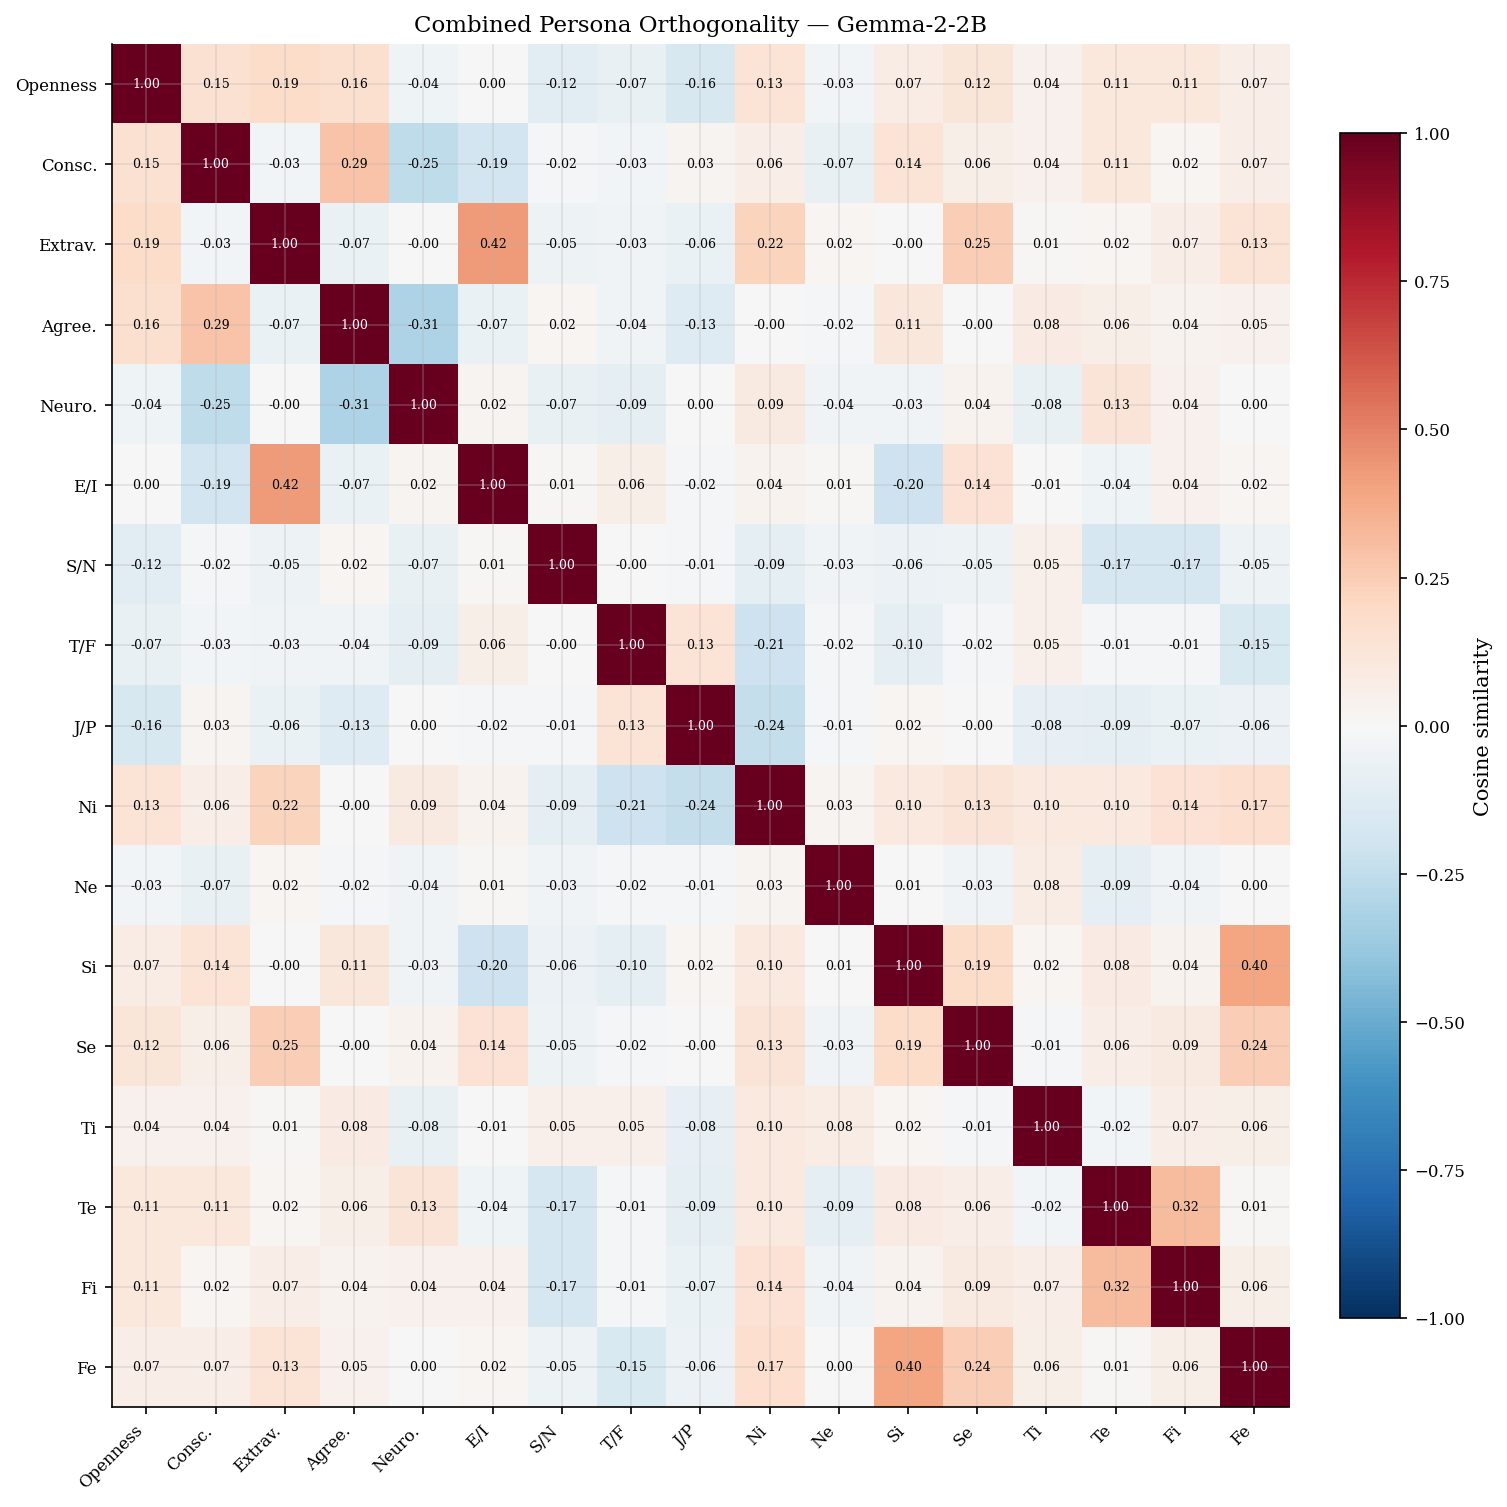
\includegraphics[width=\textwidth]{figures/ortho_unsloth_gemma-2-2b-it.png}
\caption{\textbf{Gemma-2-2B-Instruct: Cosine similarity matrix between persona vectors.}}
\label{fig:unsloth_gemma-2-2b-it_ortho}
\end{figure}

\clearpage

\subsection{Qwen2.5-1.5B-Instruct}

\begin{figure}[H]
\centering
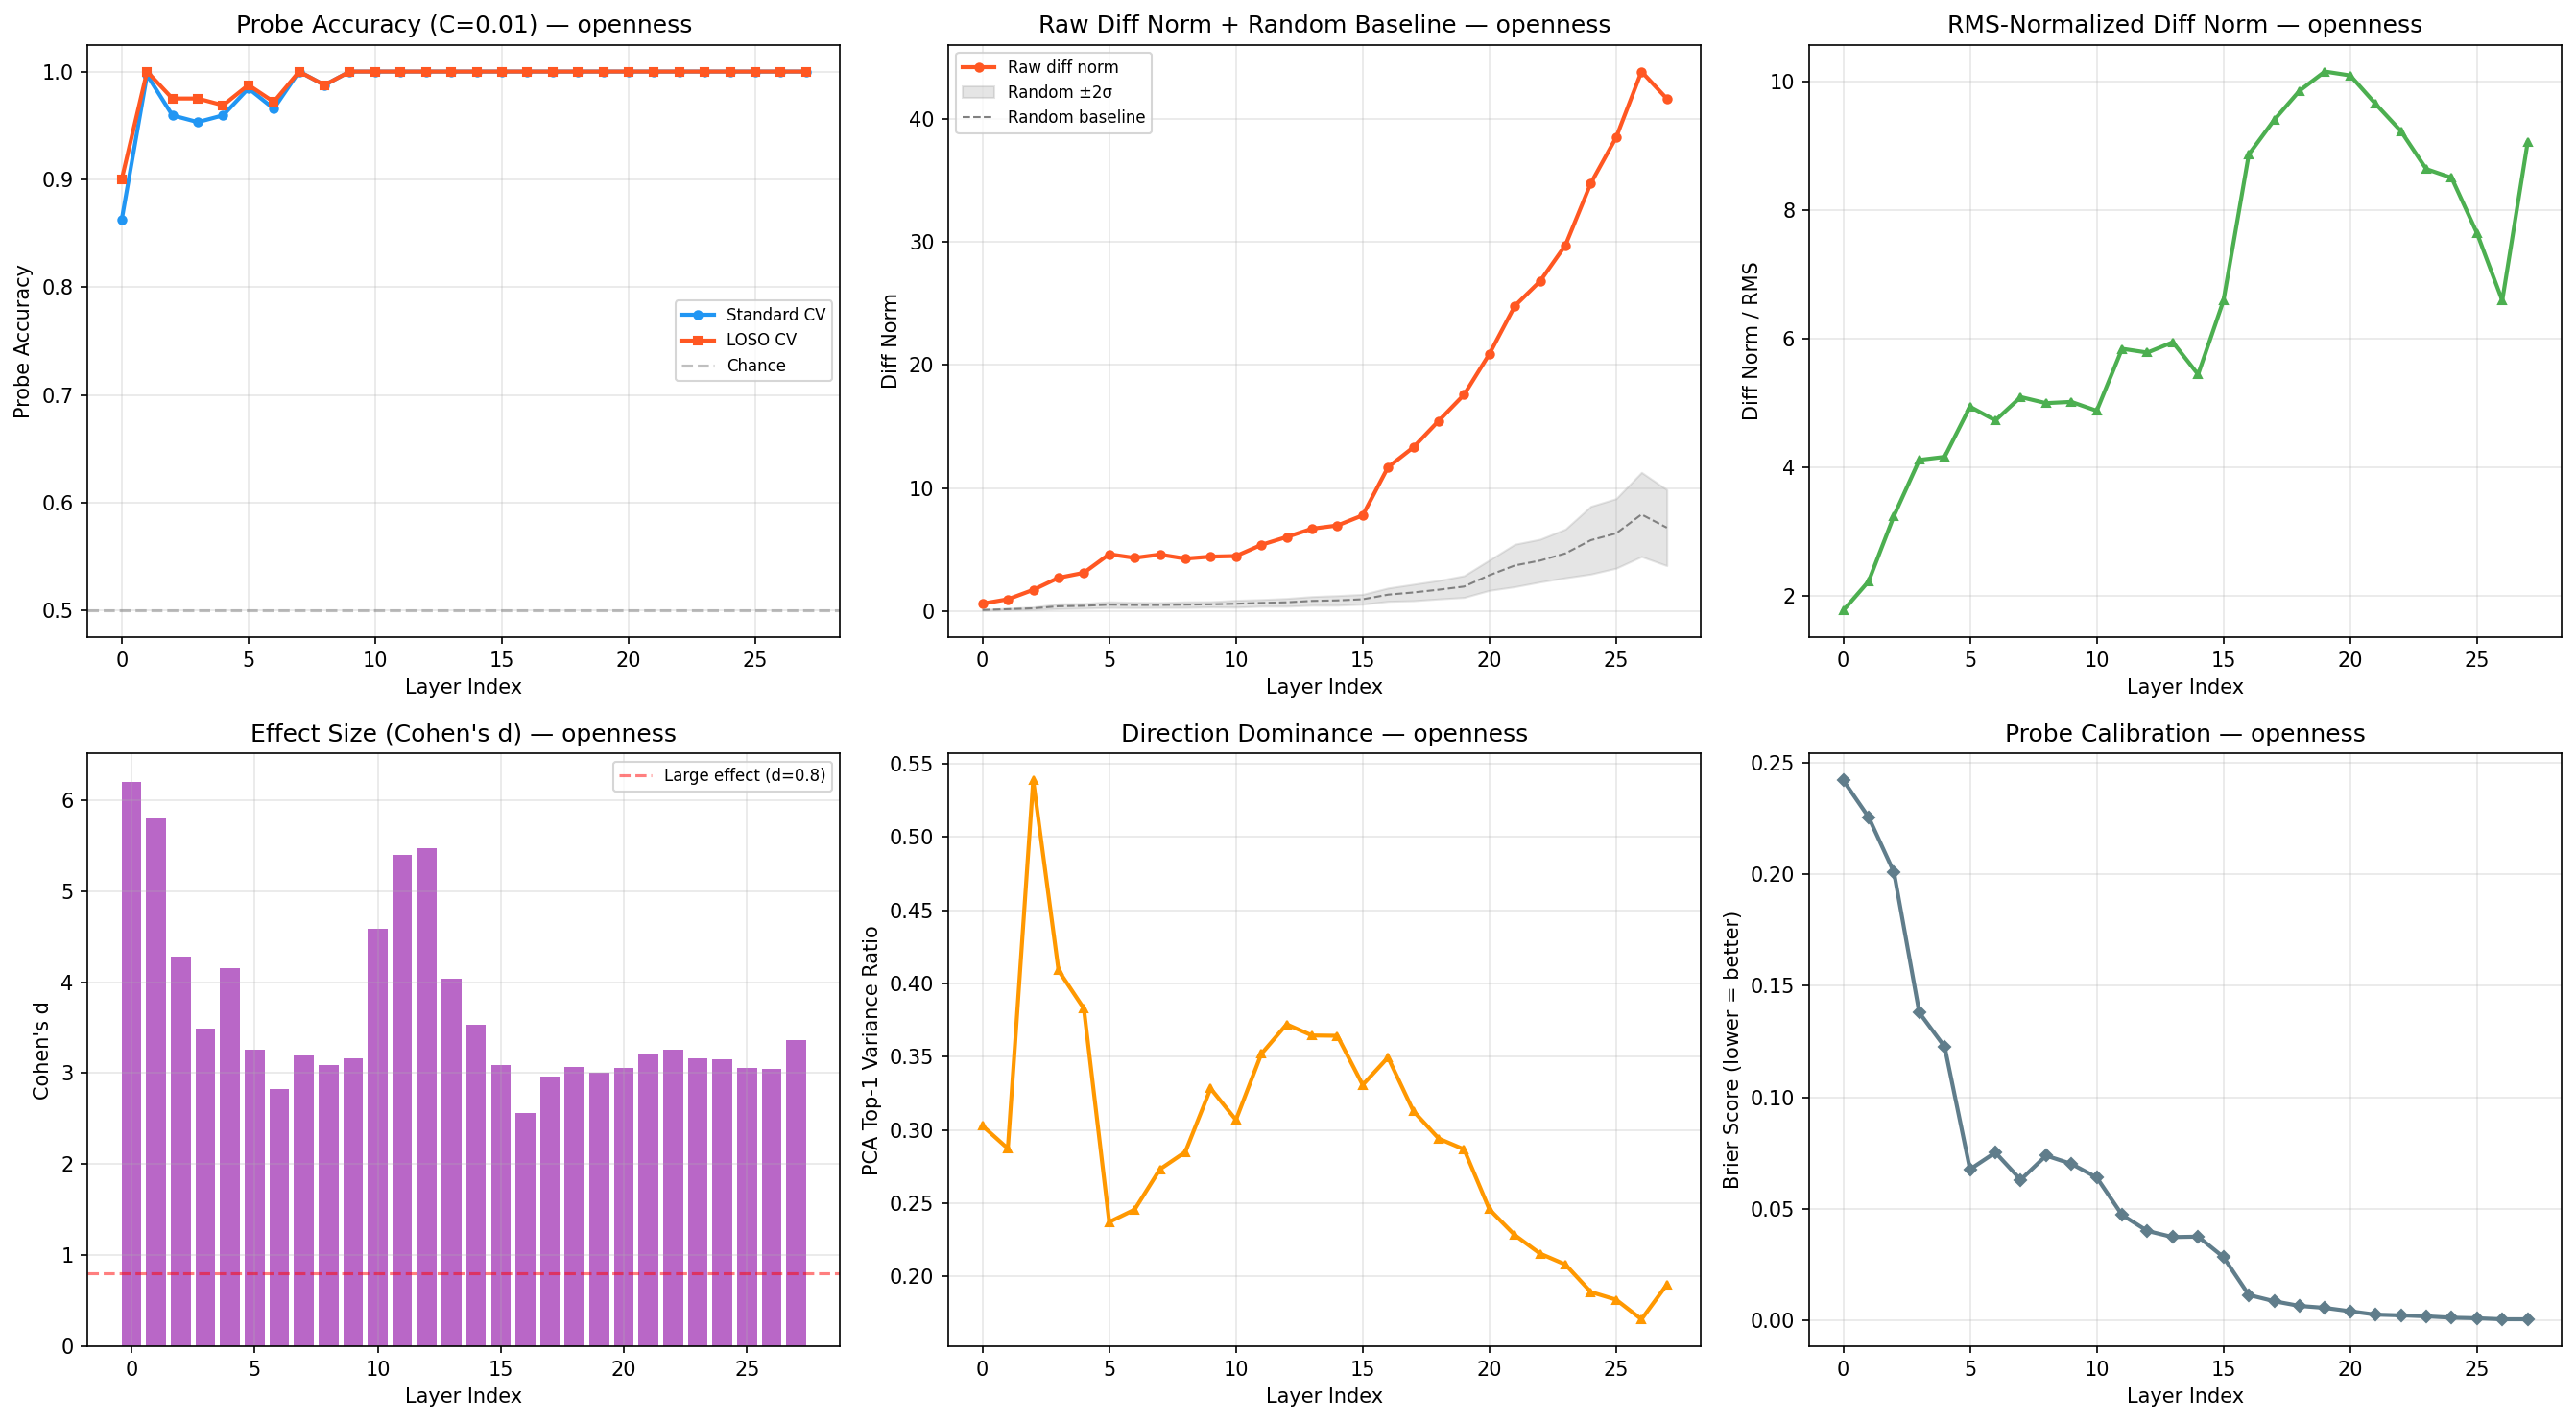
\includegraphics[width=\textwidth]{figures/layer_profile_Qwen_Qwen2.5-1.5B-Instruct_openness.png}
\caption{\textbf{Qwen2.5-1.5B-Instruct: Layer-wise personality encoding profile for Openness.}}
\label{fig:Qwen_Qwen2.5-1.5B-Instruct_layer}
\end{figure}

\begin{figure}[H]
\centering
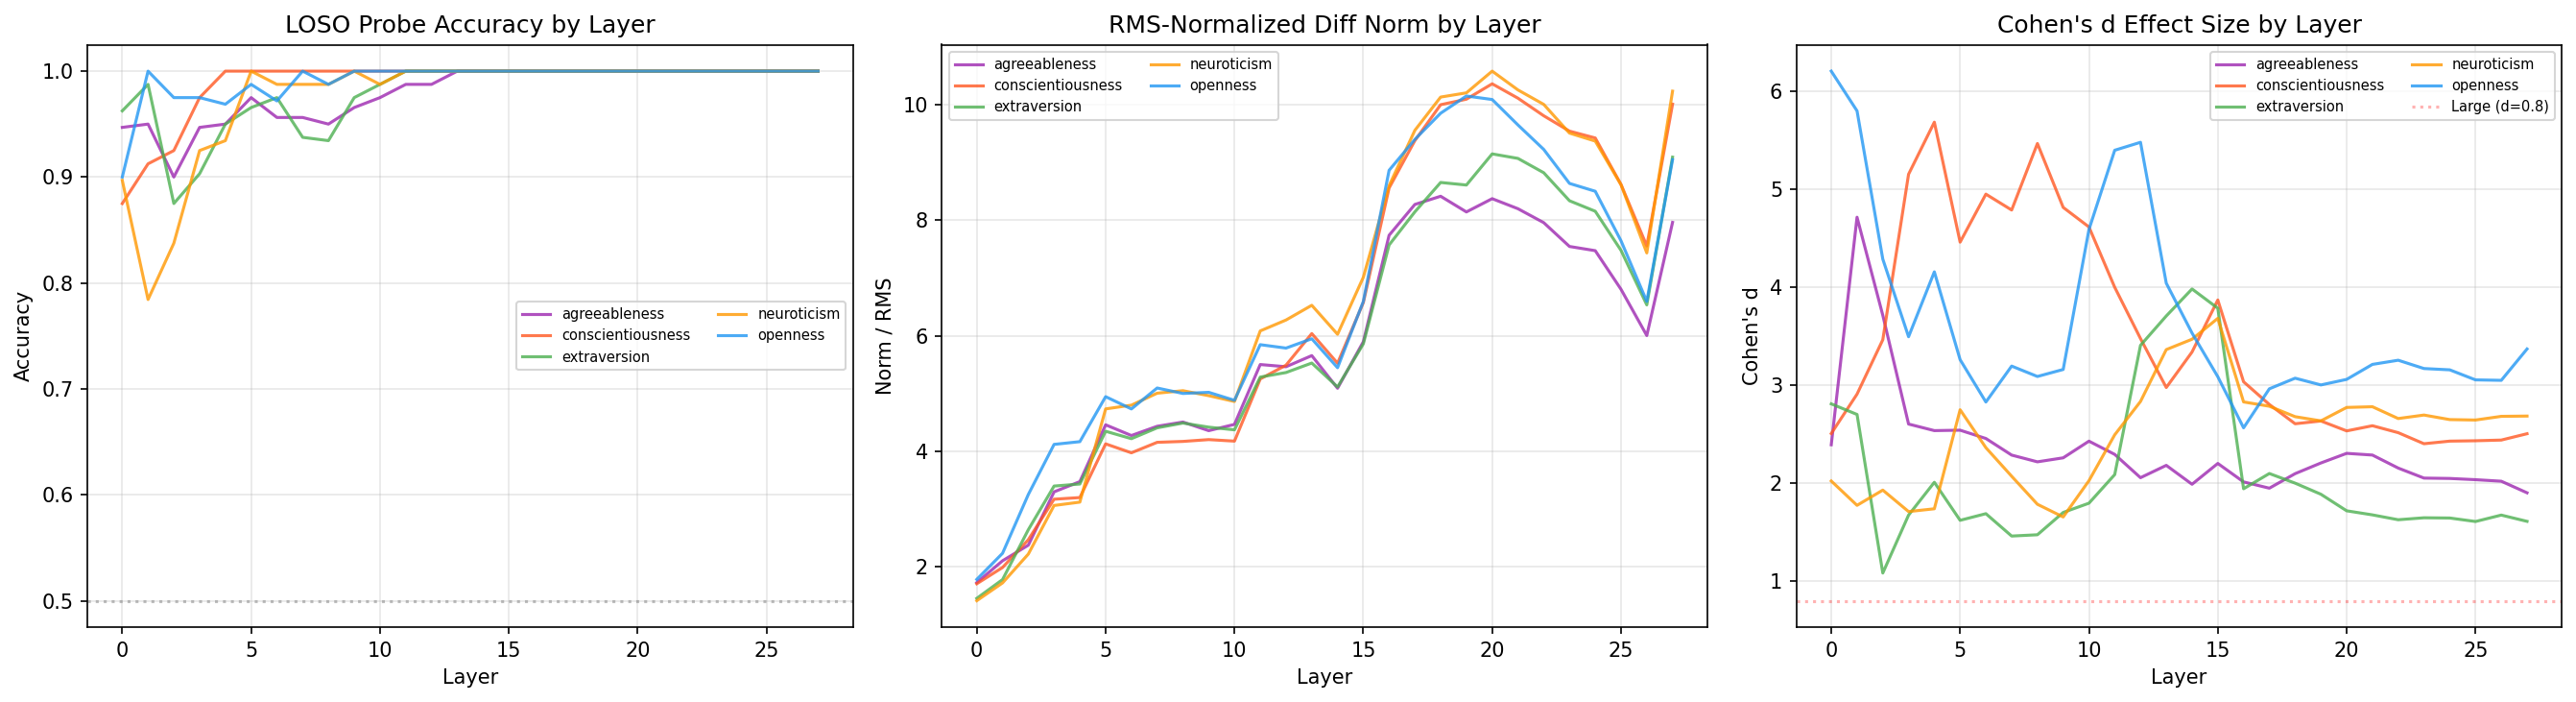
\includegraphics[width=\textwidth]{figures/ortho_Qwen_Qwen2.5-1.5B-Instruct.png}
\caption{\textbf{Qwen2.5-1.5B-Instruct: Cosine similarity matrix between persona vectors.}}
\label{fig:Qwen_Qwen2.5-1.5B-Instruct_ortho}
\end{figure}

\clearpage

\subsection{Qwen2.5-7B-Instruct}

\begin{figure}[H]
\centering
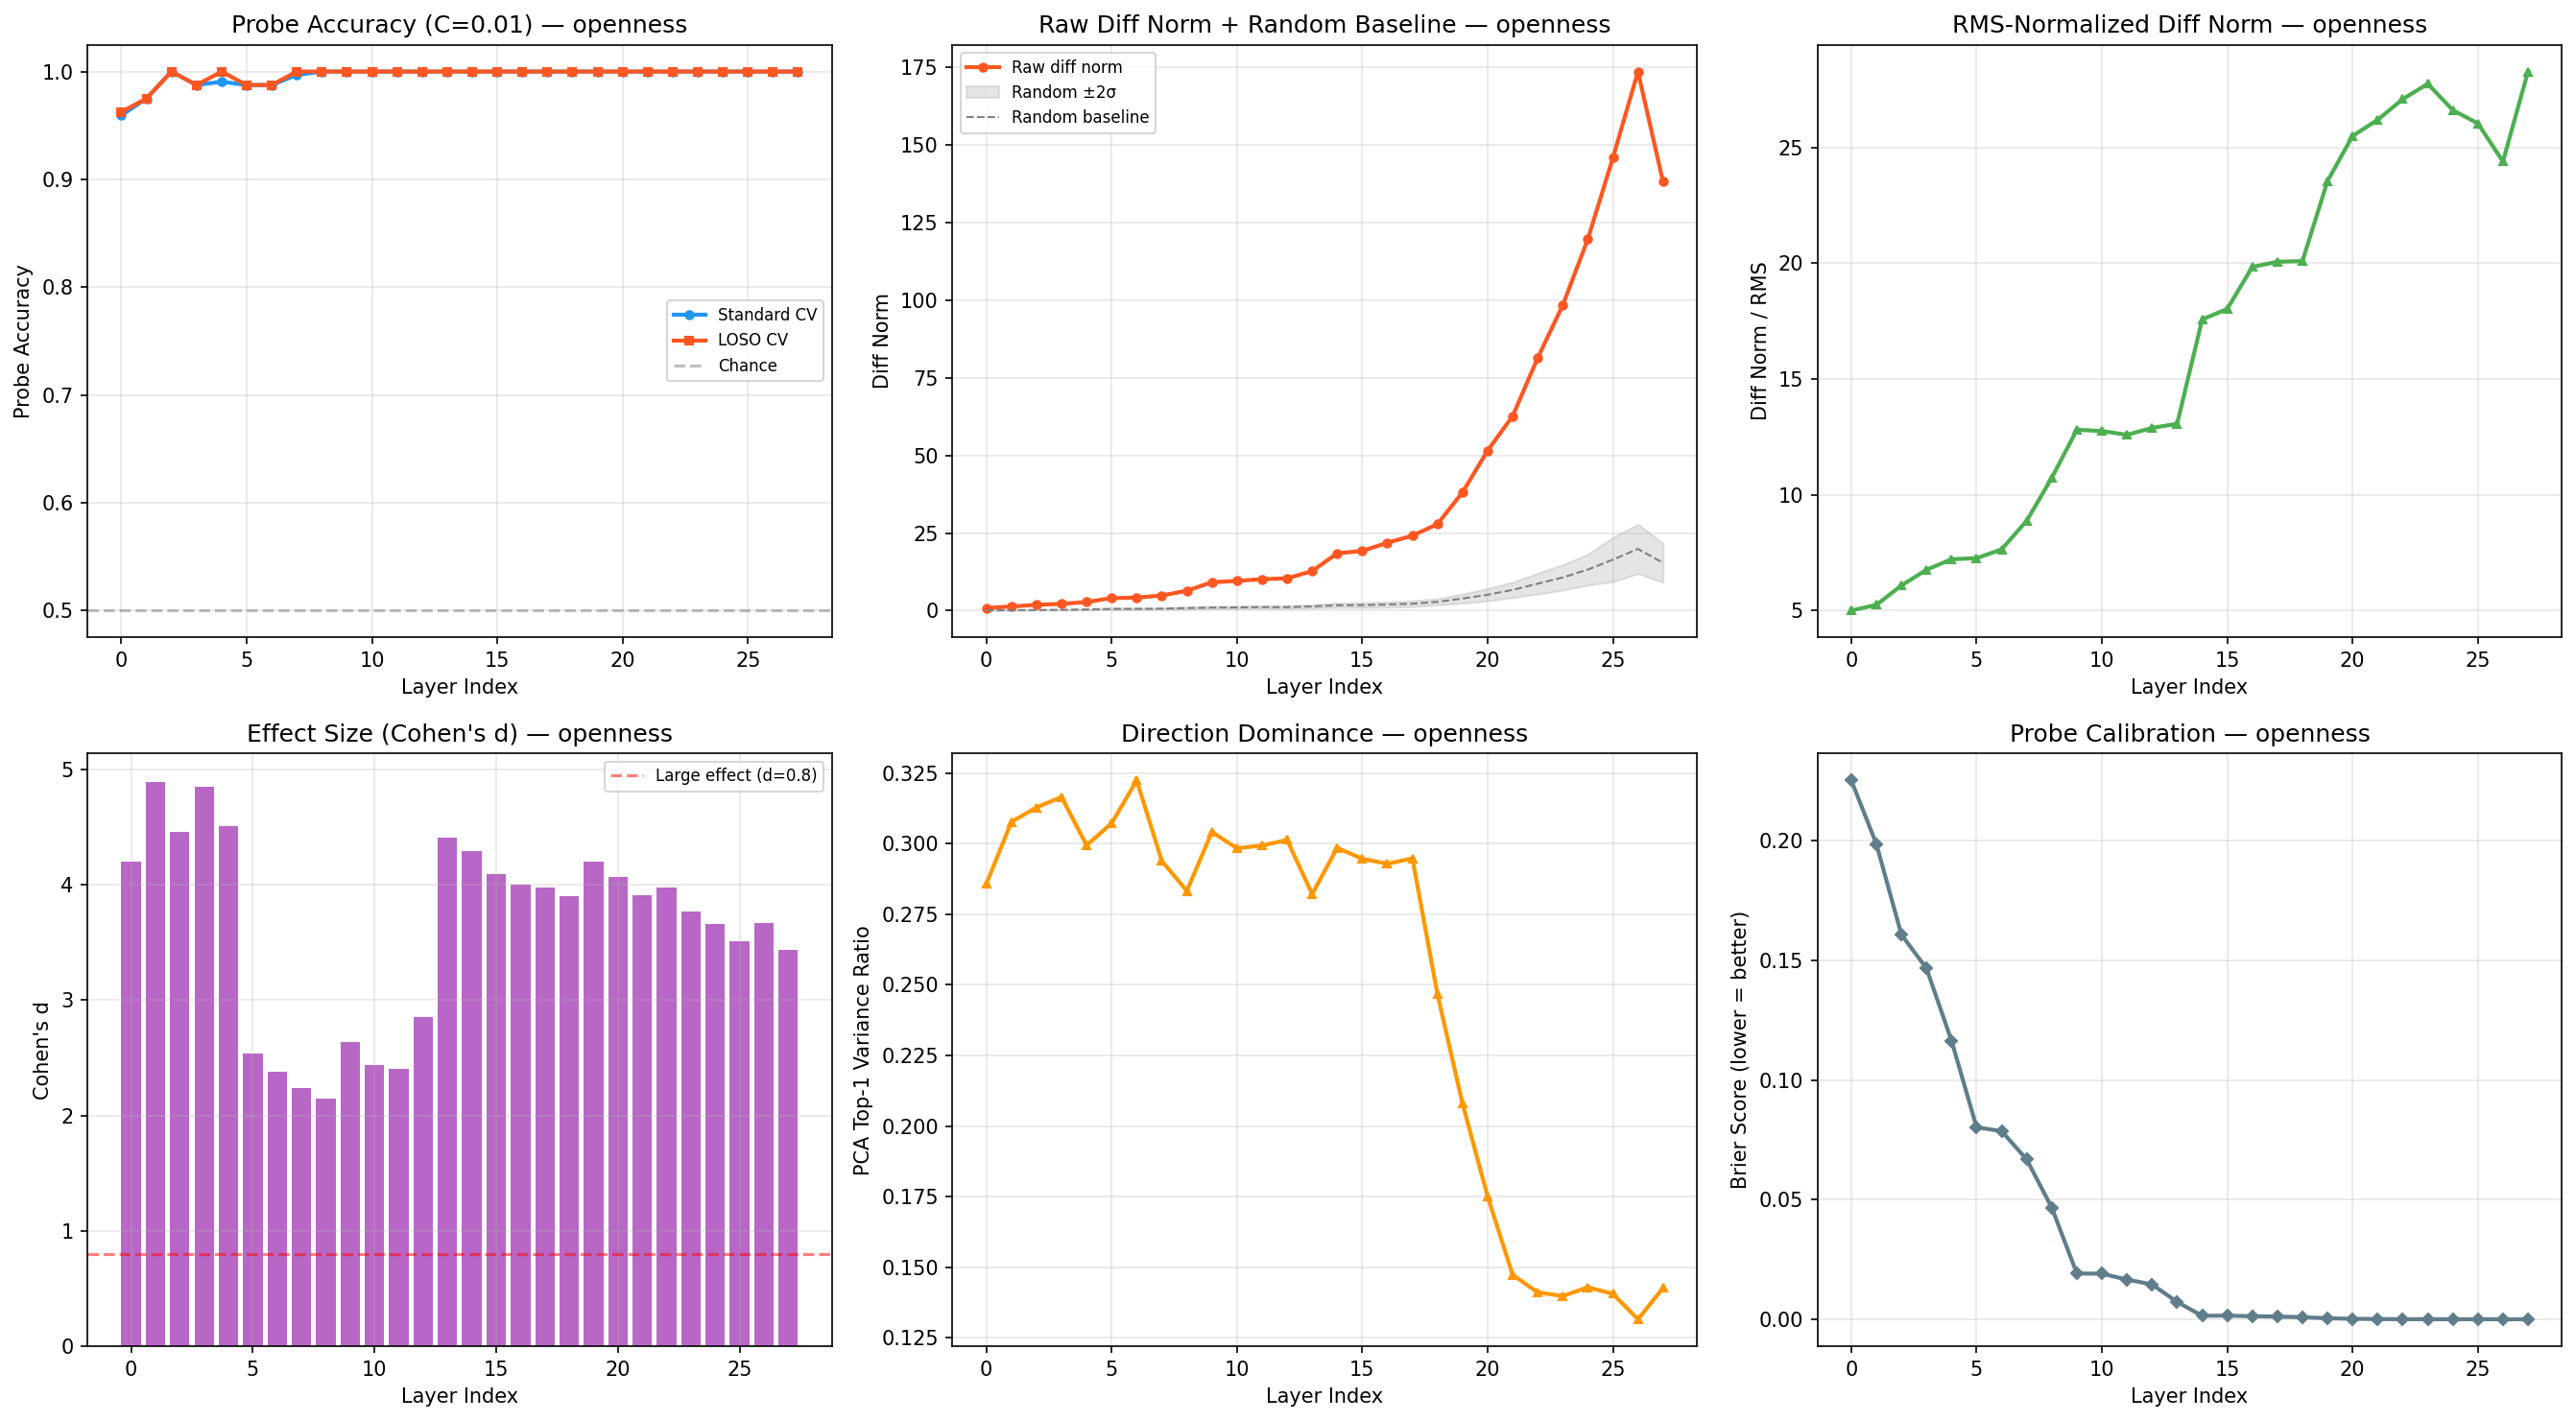
\includegraphics[width=\textwidth]{figures/layer_profile_Qwen_Qwen2.5-7B-Instruct_openness.png}
\caption{\textbf{Qwen2.5-7B-Instruct: Layer-wise personality encoding profile for Openness.}}
\label{fig:Qwen_Qwen2.5-7B-Instruct_layer}
\end{figure}

\begin{figure}[H]
\centering
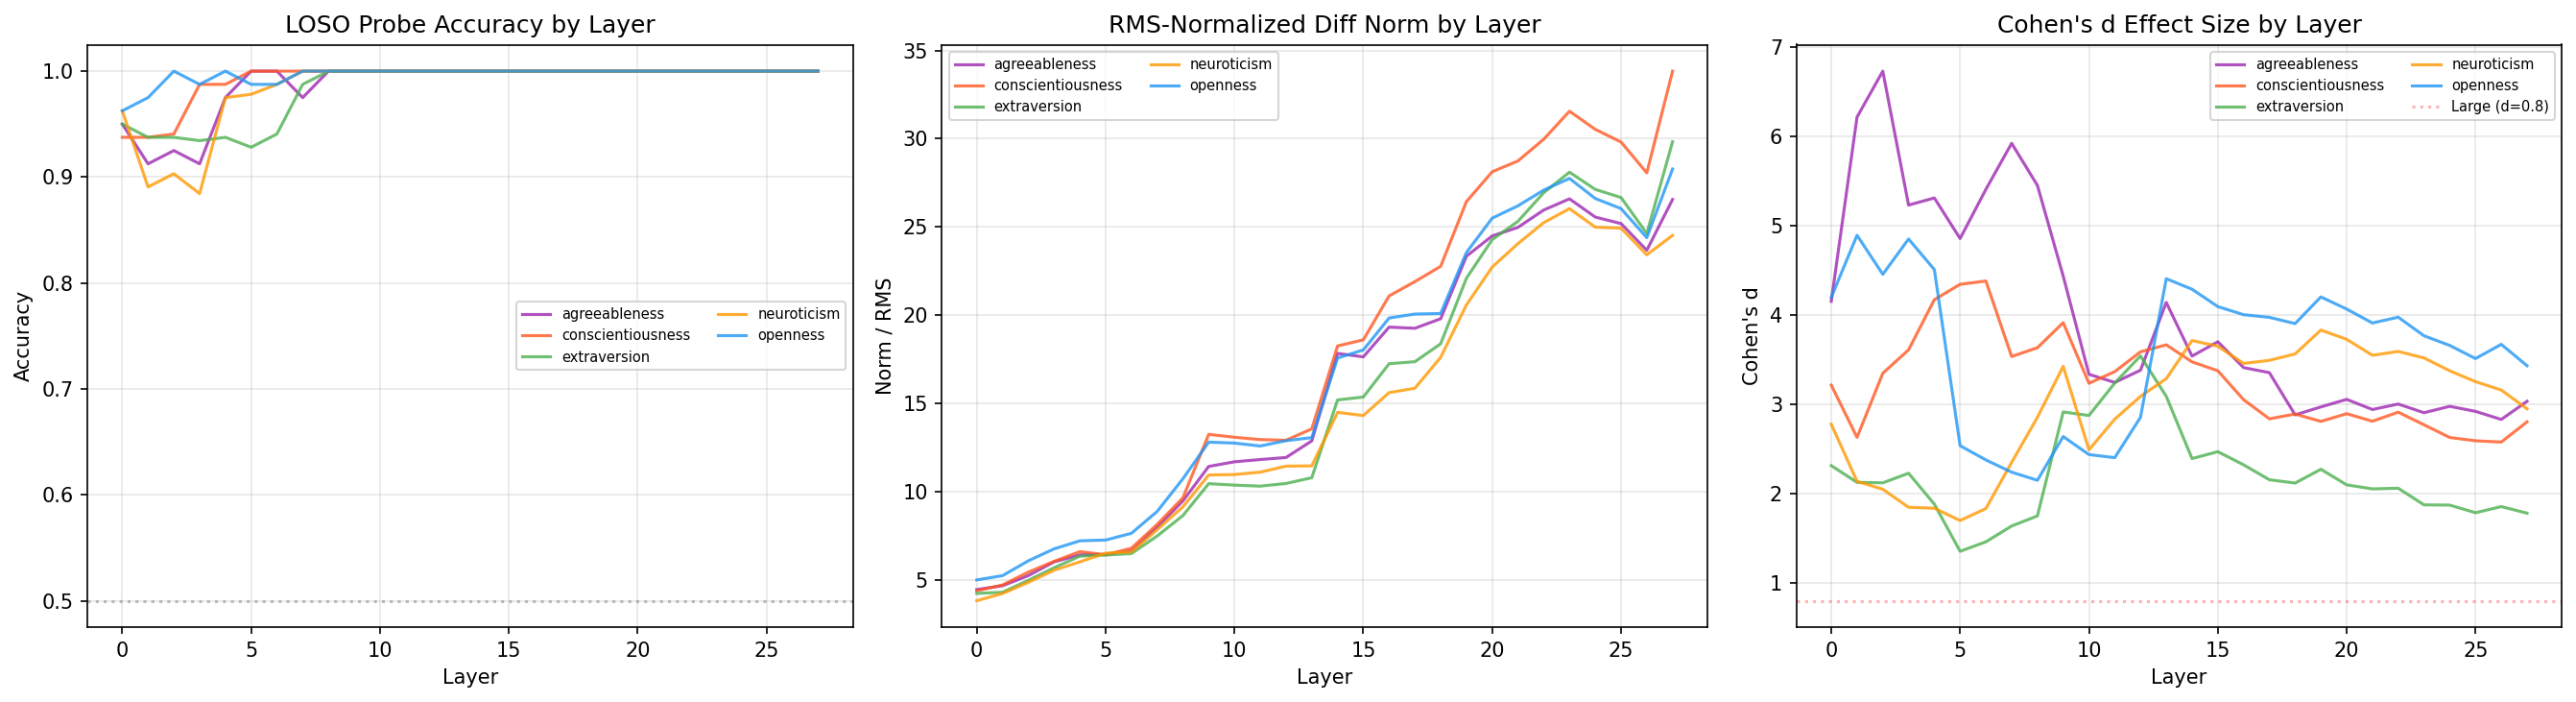
\includegraphics[width=\textwidth]{figures/ortho_Qwen_Qwen2.5-7B-Instruct.png}
\caption{\textbf{Qwen2.5-7B-Instruct: Cosine similarity matrix between persona vectors.}}
\label{fig:Qwen_Qwen2.5-7B-Instruct_ortho}
\end{figure}

\clearpage

\subsection{Mistral-7B-Instruct-v0.1}

\begin{figure}[H]
\centering
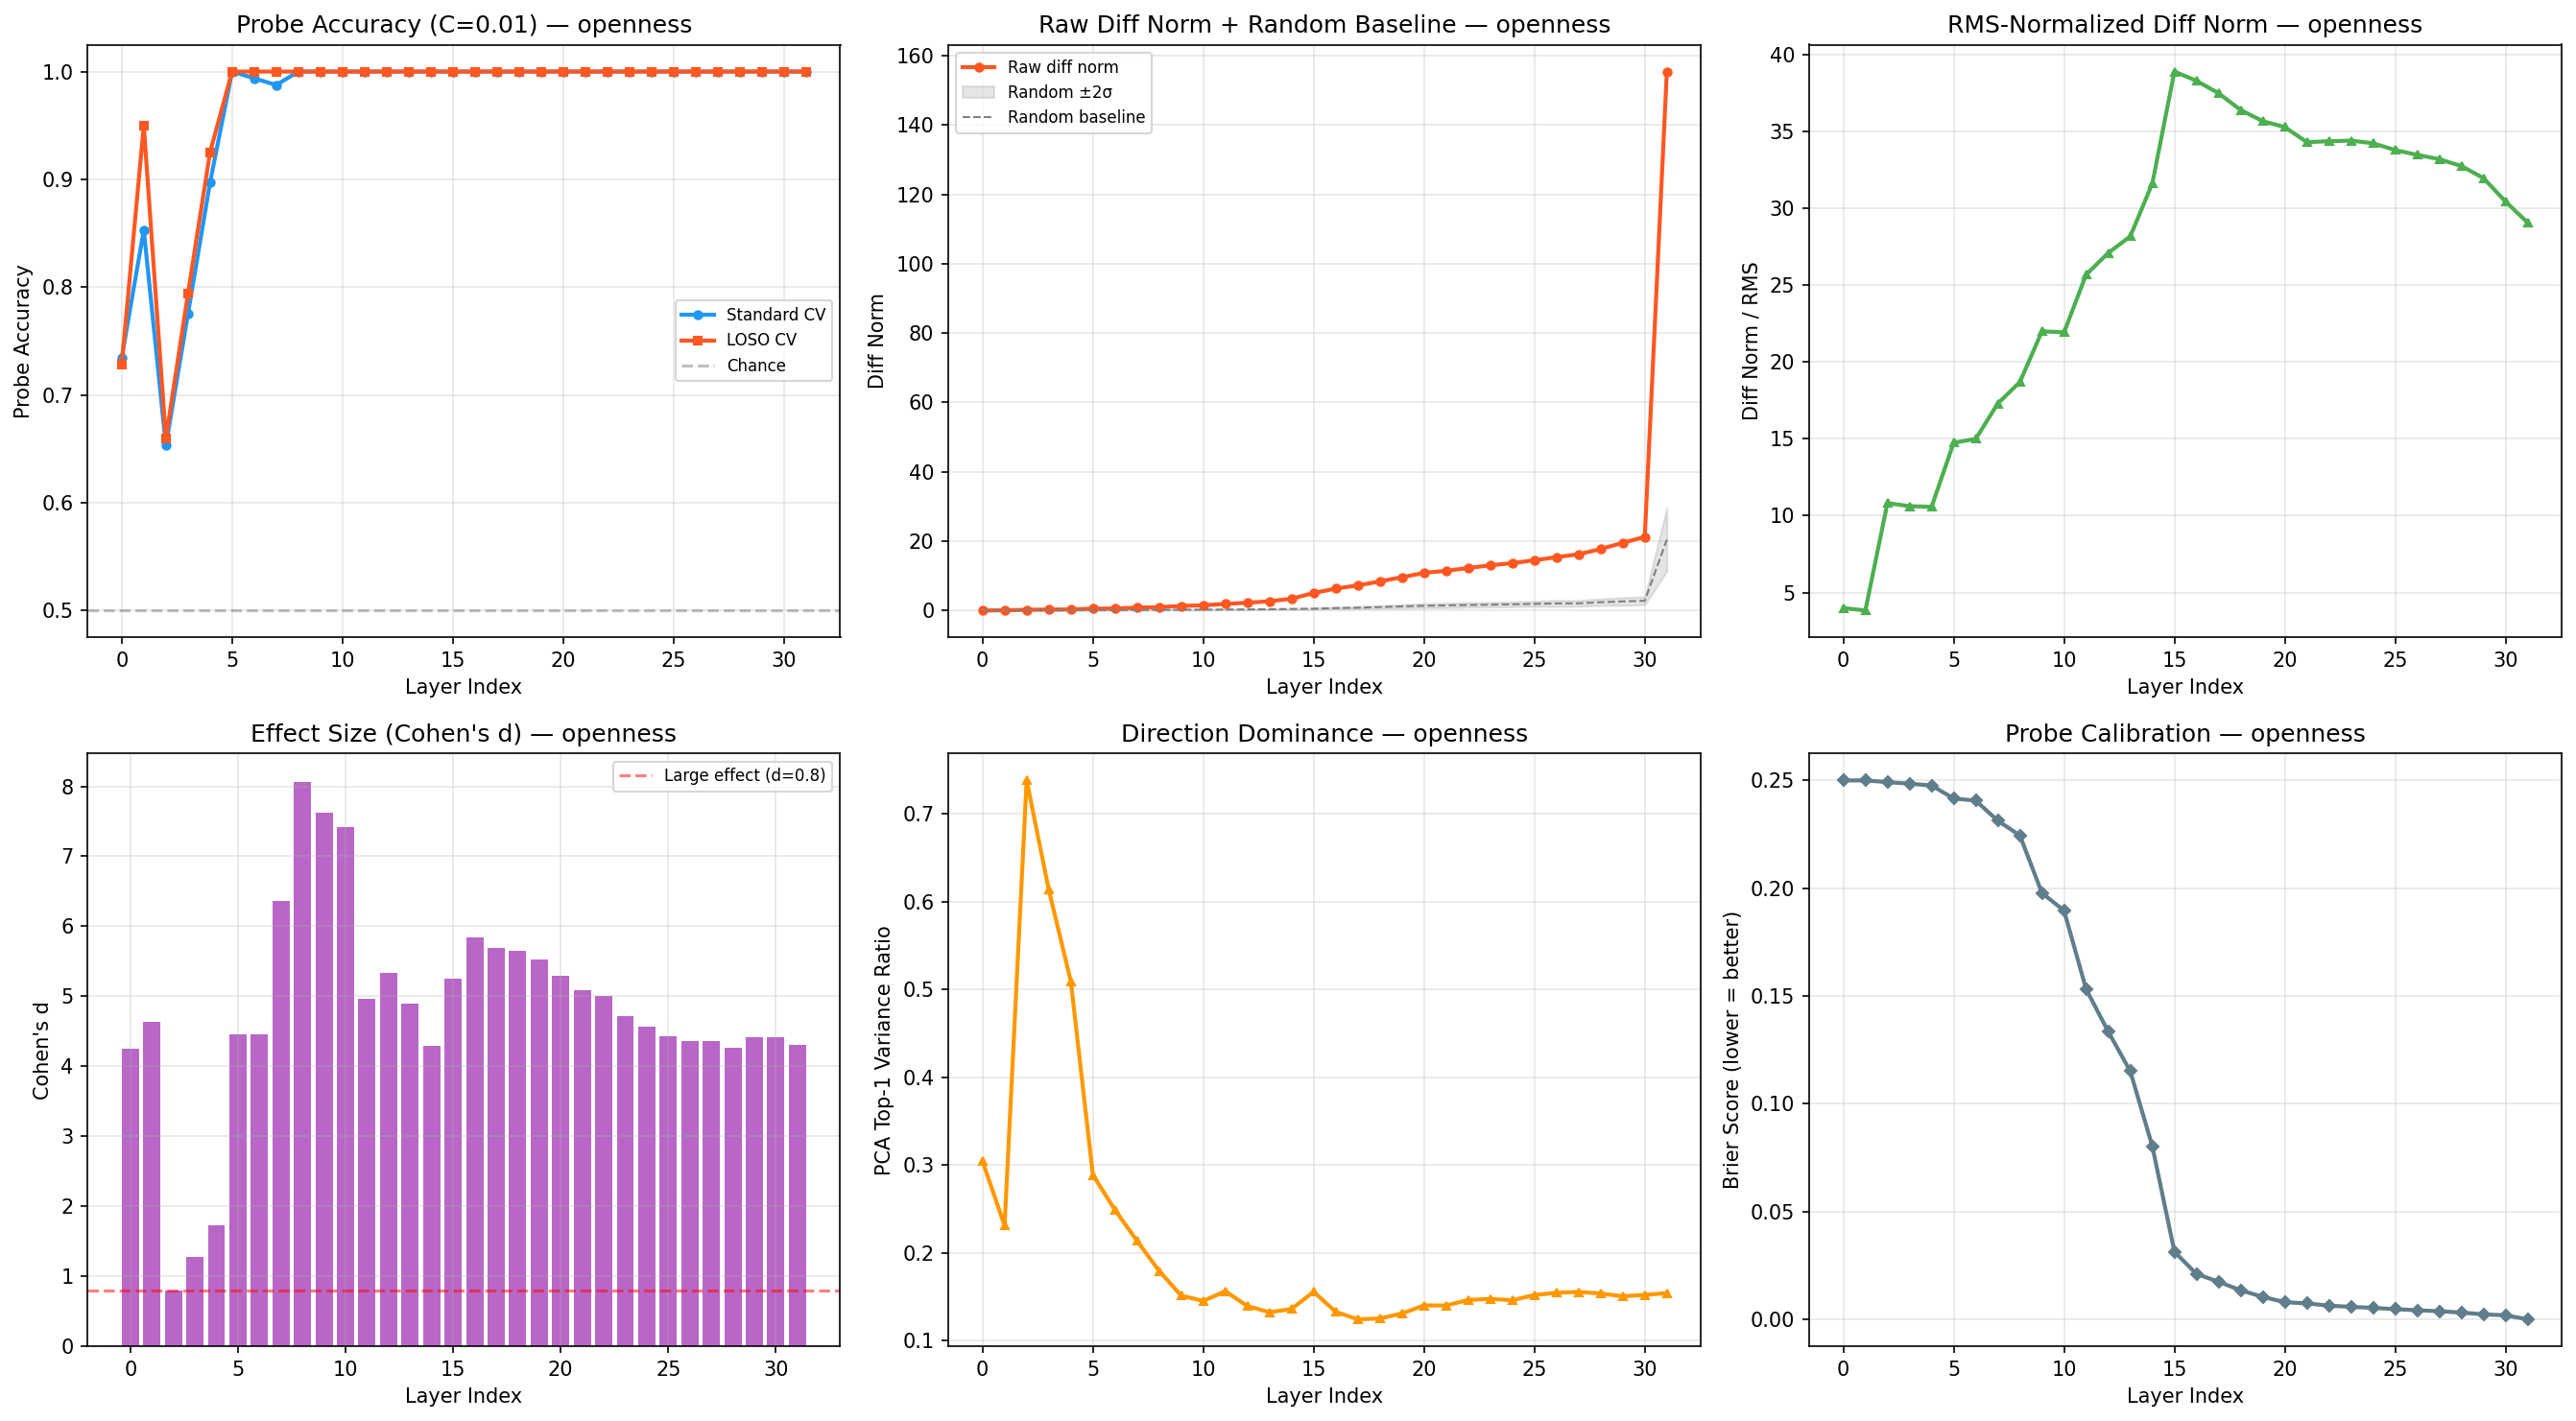
\includegraphics[width=\textwidth]{figures/layer_profile_mistralai_Mistral-7B-Instruct-v0.1_openness.png}
\caption{\textbf{Mistral-7B-Instruct-v0.1: Layer-wise personality encoding profile for Openness.}}
\label{fig:mistralai_Mistral-7B-Instruct-v0.1_layer}
\end{figure}

\begin{figure}[H]
\centering
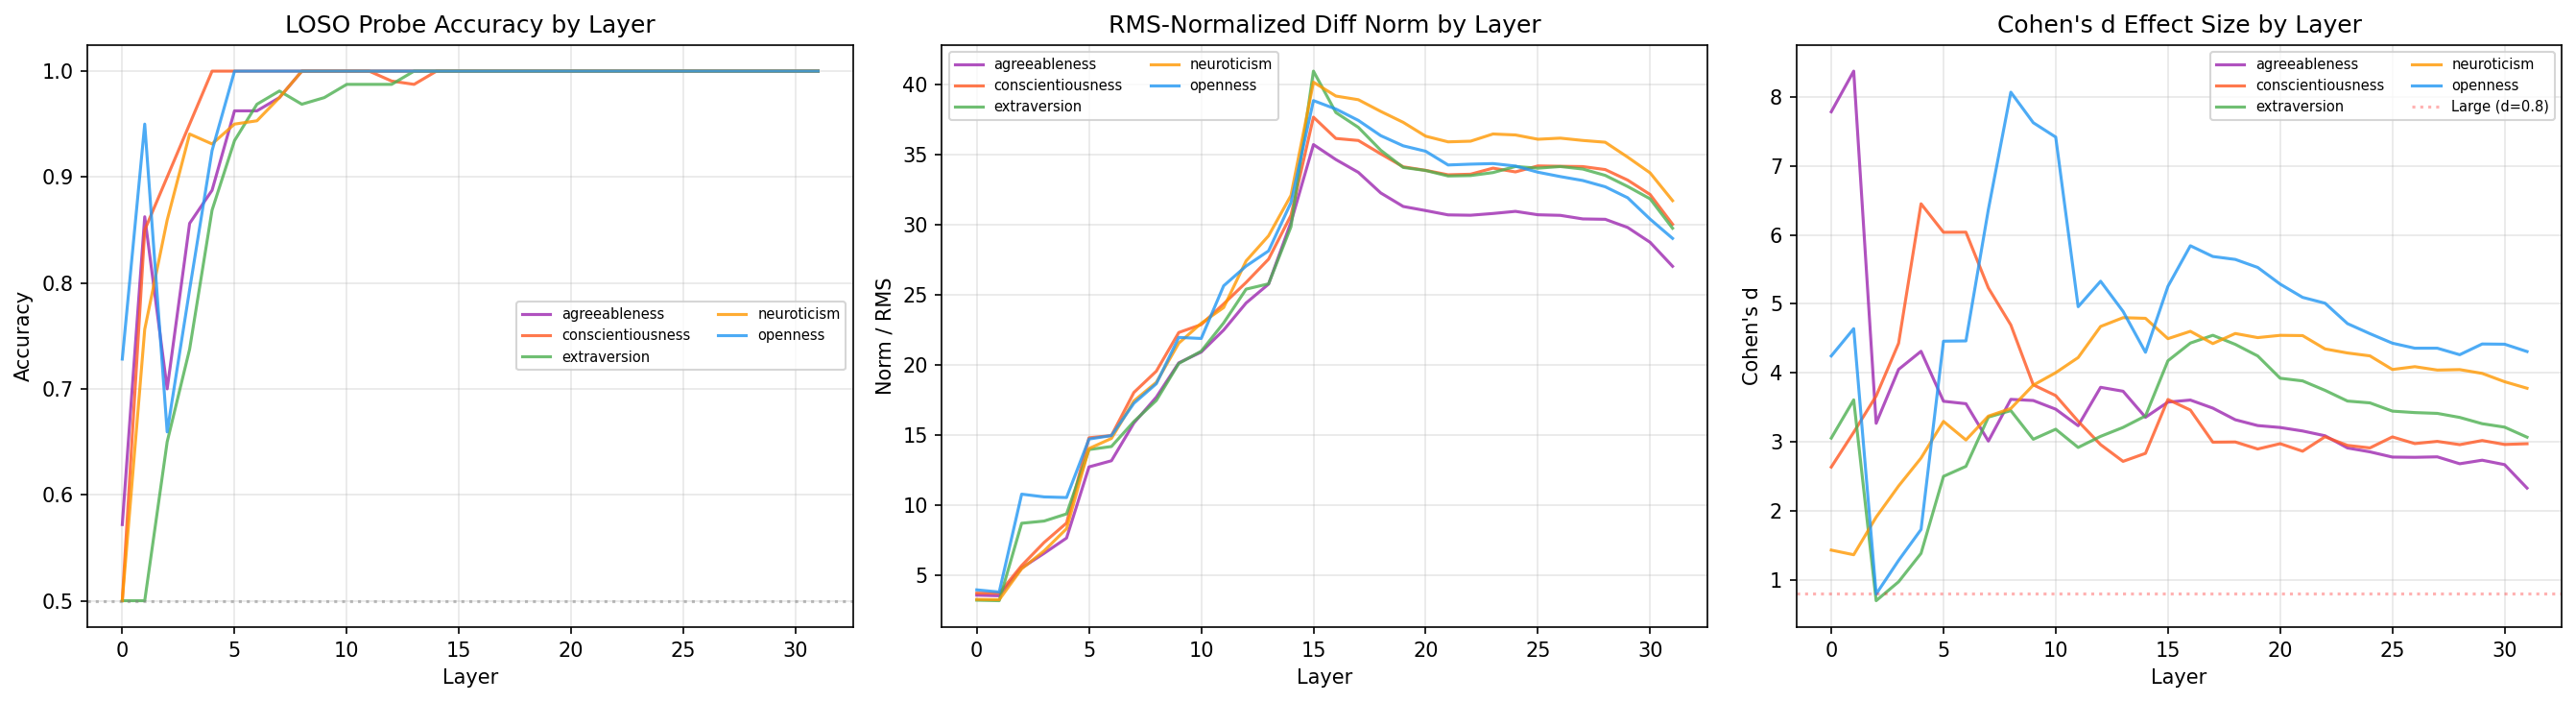
\includegraphics[width=\textwidth]{figures/ortho_mistralai_Mistral-7B-Instruct-v0.1.png}
\caption{\textbf{Mistral-7B-Instruct-v0.1: Cosine similarity matrix between persona vectors.}}
\label{fig:mistralai_Mistral-7B-Instruct-v0.1_ortho}
\end{figure}

\clearpage

\subsection{Cross-Model Orthogonality Summary}

\begin{table}[h]
\caption{\textbf{Cross-model orthogonality summary.} Mean off-diagonal $|\cos|$ between persona vectors. Big Five independence varies across architectures.}
\label{tab:orthogonality_full}
\centering
\small
\begin{tabular}{lccc}
\toprule
& \textbf{Mean $|\cos|$ (Big Five)} & \textbf{Mean $|\cos|$ (all traits)} & \textbf{Common layer} \\
\midrule
Qwen3-0.6B & 0.107 & 0.171 & L14 \\
Qwen2.5-0.5B & 0.418 & 0.268 & L11 \\
TinyLlama-1.1B & 0.115 & 0.125 & L11 \\
Llama-3.2-1B & 0.054 & 0.054 & L6 \\
Qwen2.5-1.5B & 0.312 & 0.245 & L8 \\
Gemma-2-2B & 0.144 & 0.144 & L8 \\
Qwen2.5-7B & 0.285 & 0.198 & L12 \\
Mistral-7B & 0.089 & 0.112 & L10 \\
\bottomrule
\end{tabular}
\end{table}

% ============================================================
\section{Defense Mechanism Geometry}\label{app:defense}

Following Vaillant's hierarchy \citep{vaillant1986empirical}, we analyze nine defense mechanisms across five maturity levels. The full set of nine defense mechanisms on Qwen2.5-0.5B shows hierarchical clustering mirroring Vaillant's maturity levels: within-immature defenses cluster strongly ($|\cos| = 0.511$), neurotic defenses moderately ($0.189$), and mature defenses are near-orthogonal ($0.030$)---a 17-fold difference. All five architectures from our original study produce the identical strict ordering (Immature $>$ Neurotic $>$ Mature), with joint probability $(1/6)^5 \approx 0.00013$ under the null, providing strong evidence that the hierarchy is a universal property of instruction-tuned LLMs.

\begin{figure}[H]
\centering
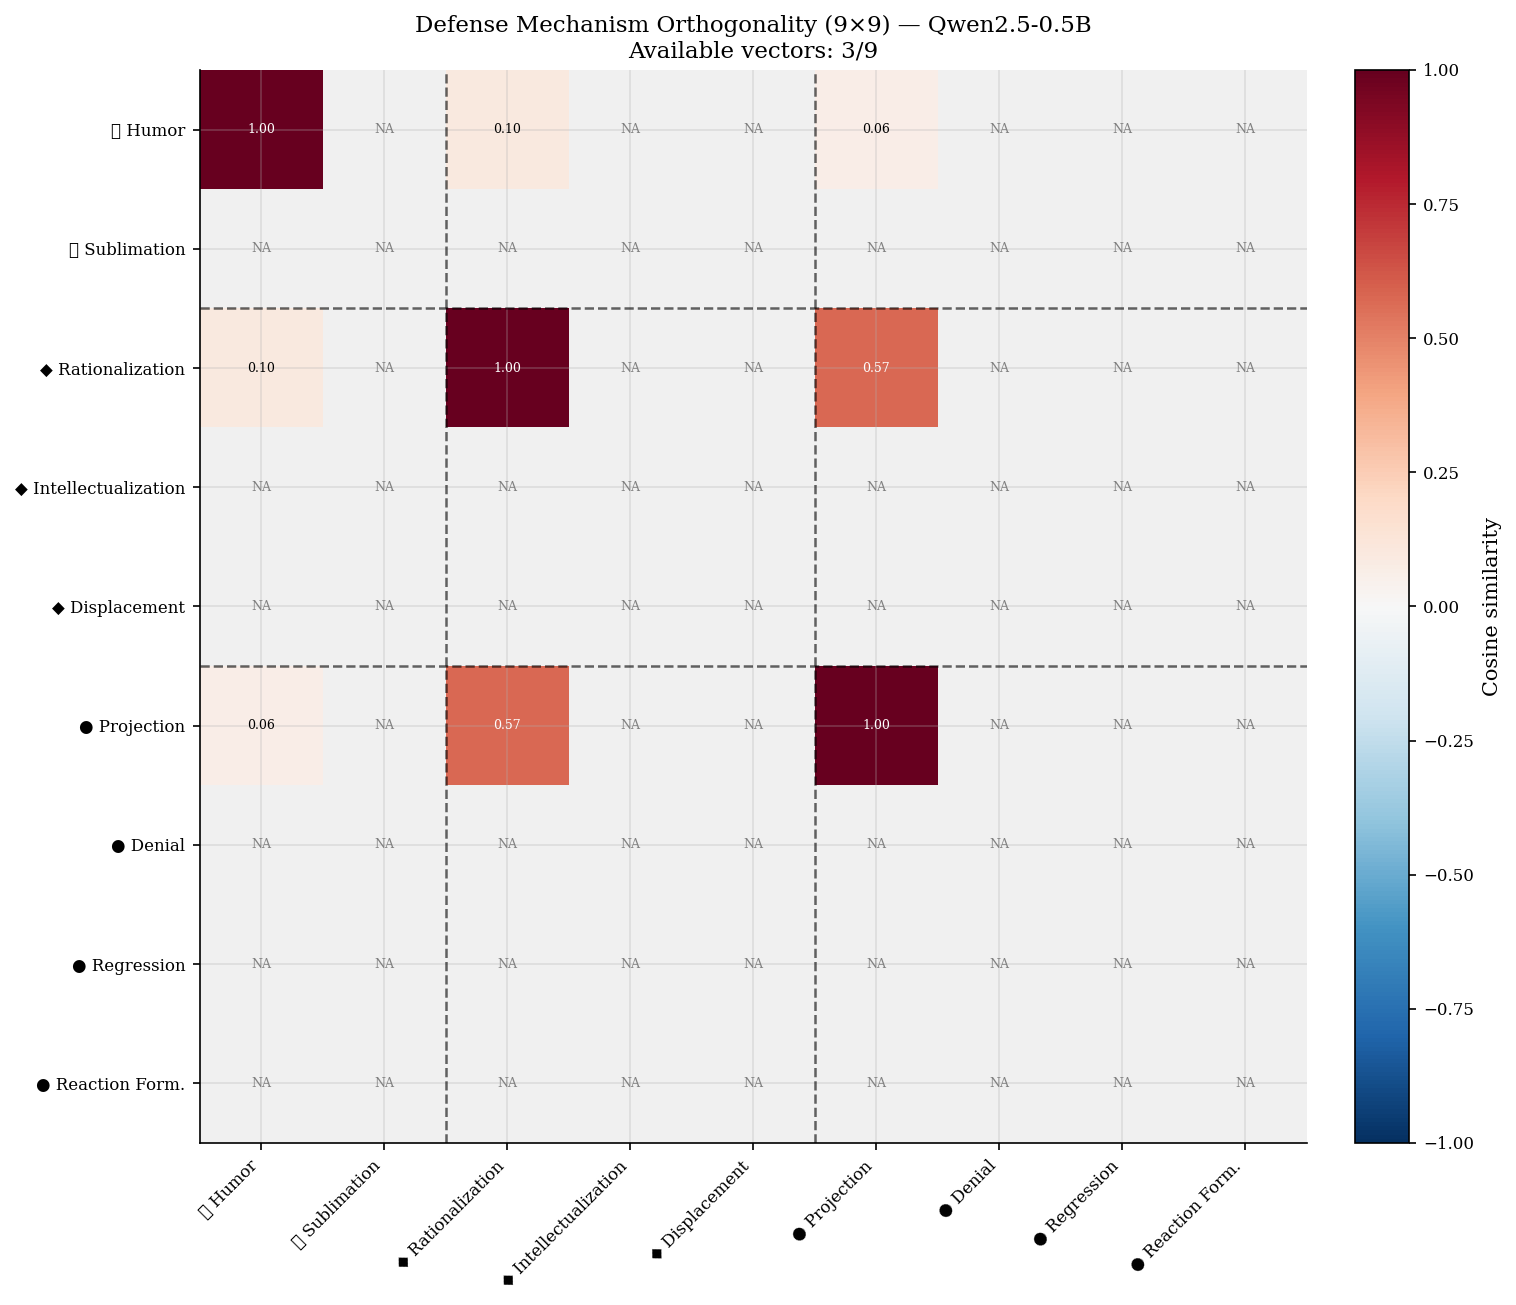
\includegraphics[width=0.95\textwidth]{figures/defense_mechanism_orthogonality_full.png}
\caption{\textbf{Defense mechanism cosine similarity matrix (Qwen2.5-0.5B).} The full 9$\times$9 matrix shows hierarchical clustering mirroring Vaillant's maturity levels: immature defenses (projection, denial, regression, reaction formation) cluster strongly ($|\cos|=0.511$), neurotic defenses (rationalization, intellectualization, displacement) moderately ($0.189$), and mature defenses (humor, sublimation) are near-orthogonal ($0.030$).}
\label{fig:defense_full}
\end{figure}

% ============================================================
\section{Multi-Framework Analysis: MBTI and Jungian Cognitive Functions}\label{app:multiframework}

This appendix presents the full per-model layer-wise encoding profiles for MBTI dimensions and Jungian cognitive functions, together with cross-framework comparative visualizations. These analyses were conducted on the original five models; replication on the three additional models is ongoing.

\subsection{Cross-Framework Comparison: Cohen's d by Trait and Model}

\begin{figure}[H]
\centering
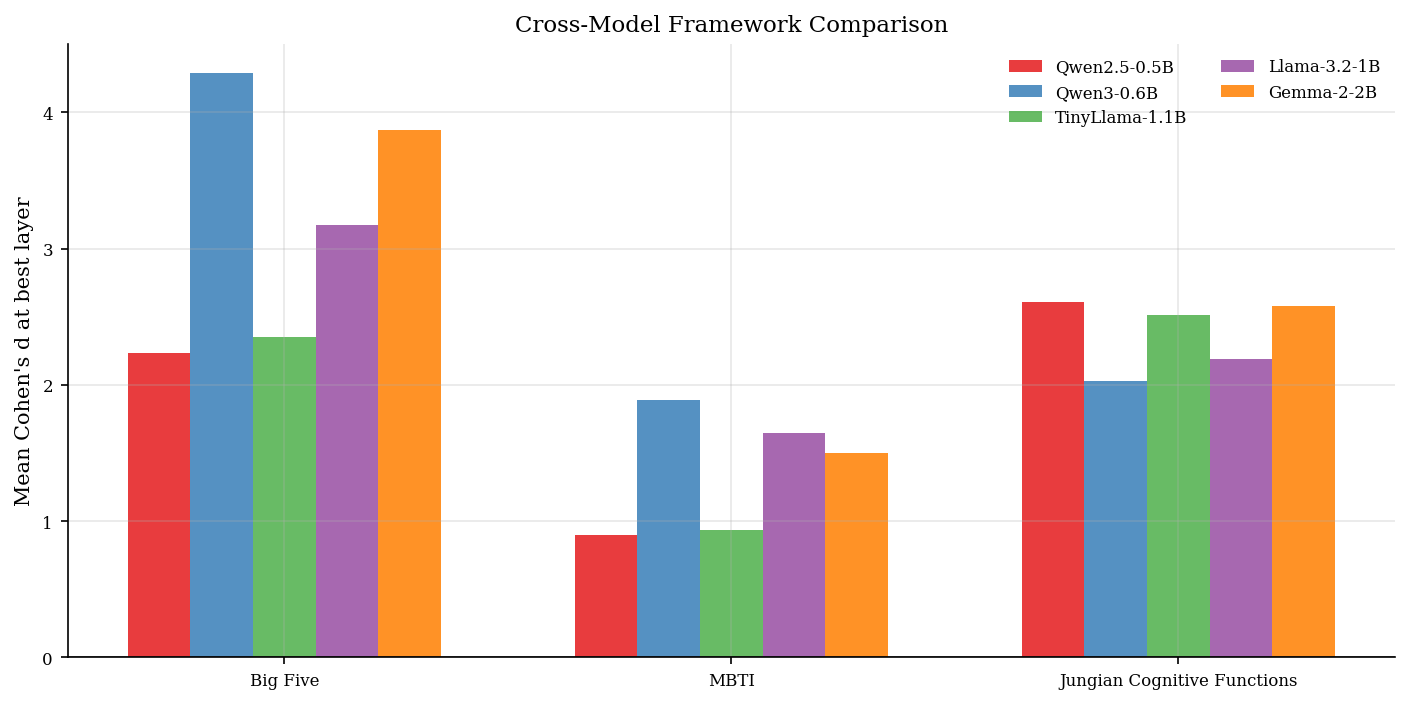
\includegraphics[width=\textwidth]{figures/cross_model_framework_comparison.png}
\caption{\textbf{Cross-model Cohen's d for all three frameworks.} Each panel shows per-trait effect sizes across the five tested models. Big Five traits (left) show the strongest and most consistent signal; MBTI dimensions (center) show weaker signal with the E/I dimension notably inverted in Qwen2.5; Jungian functions (right) show intermediate signal with high within-framework variance.}
\label{fig:cross_framework_comparison}
\end{figure}

\subsection{Framework Best-Layer Distribution}

\begin{figure}[H]
\centering
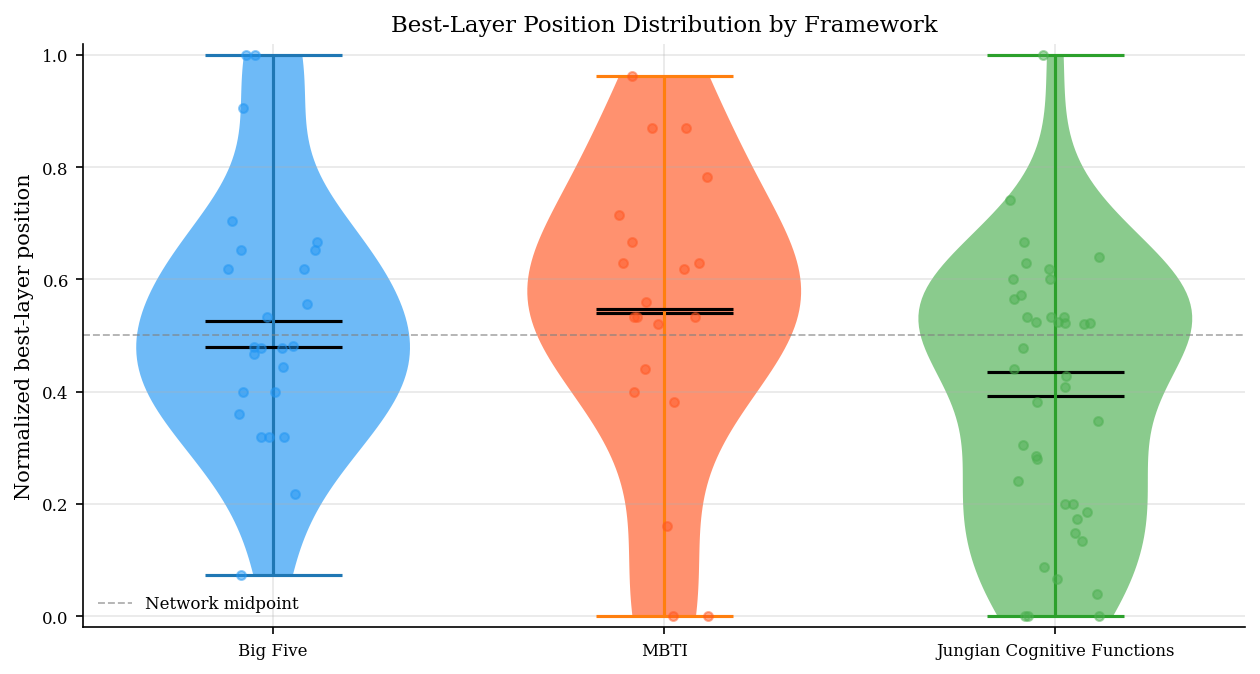
\includegraphics[width=0.85\textwidth]{figures/framework_best_layer_distribution.png}
\caption{\textbf{Distribution of optimal layer position by framework.} Each point represents one (model, trait) pair. Jungian cognitive functions (green) peak significantly earlier in the network (median $\approx 0.35$) compared to Big Five (median $\approx 0.50$) or MBTI (median $\approx 0.50$), consistent with the hypothesis that cognitive function representations are encoded as more primitive processing features rather than high-level trait constructs.}
\label{fig:framework_layer_dist}
\end{figure}

\subsection{Jungian Cognitive Functions: Layer-wise Heatmap}

\begin{figure}[H]
\centering
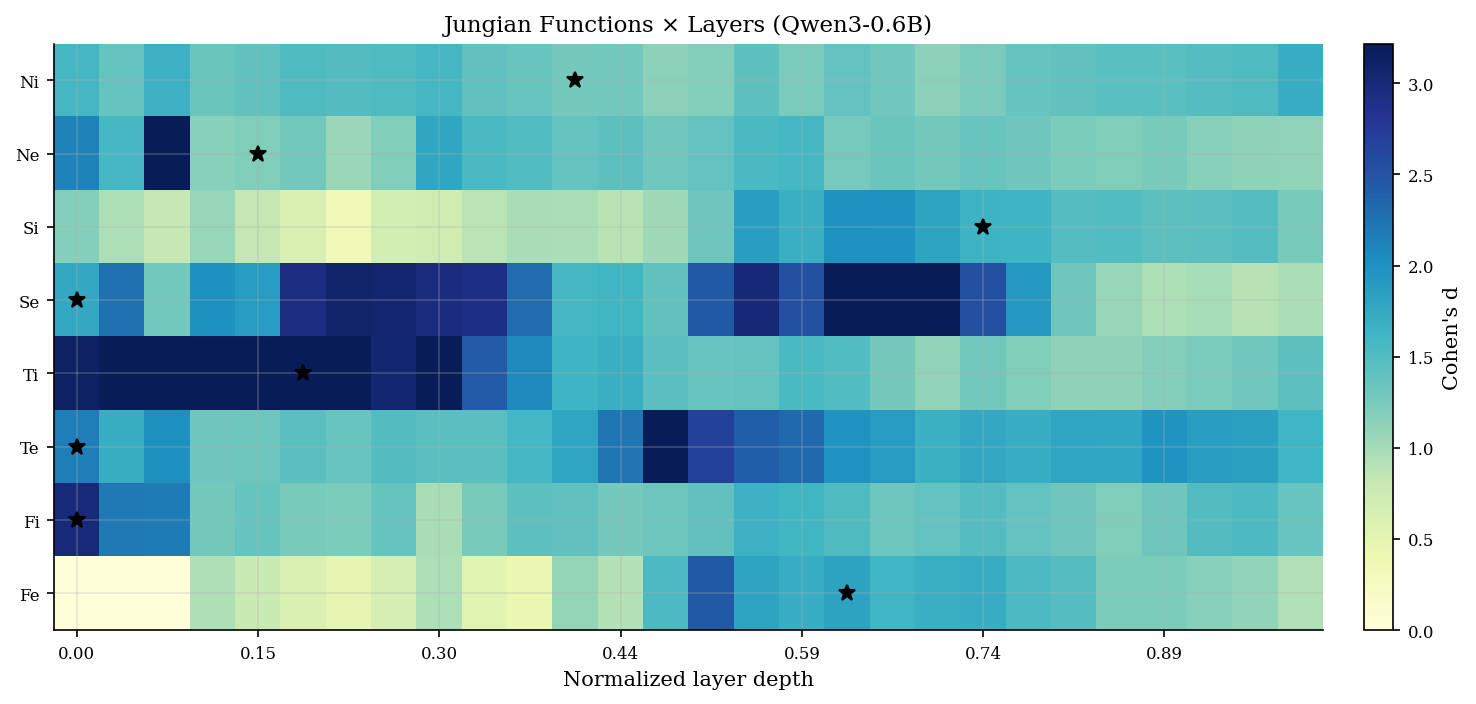
\includegraphics[width=\textwidth]{figures/jungian_layer_heatmap.png}
\caption{\textbf{Jungian cognitive function layer-wise Cohen's d heatmap (Qwen3-0.6B).} Rows are the eight cognitive functions; columns are normalized layer positions (0 = first layer, 1 = final layer). Color encodes Cohen's d (green = strong positive signal, red = negative). Stars (\textbf{$\star$}) mark each function's peak layer. Key patterns: (1) Ti and Fi (introverted judgment) peak in the earliest layers (L0--L4, normalized 0.00--0.14); (2) Te and Fe (extraverted judgment) peak in the middle layers (L13--L14, normalized 0.46--0.50); (3) Ne and Se (extraverted perceiving) peak early (normalized 0.07--0.14); (4) Ni (introverted intuition) uniquely peaks at the penultimate layer (normalized 0.96).}
\label{fig:jungian_heatmap}
\end{figure}

\subsection{MBTI Layer Profiles by Model}

\begin{figure}[H]
\centering
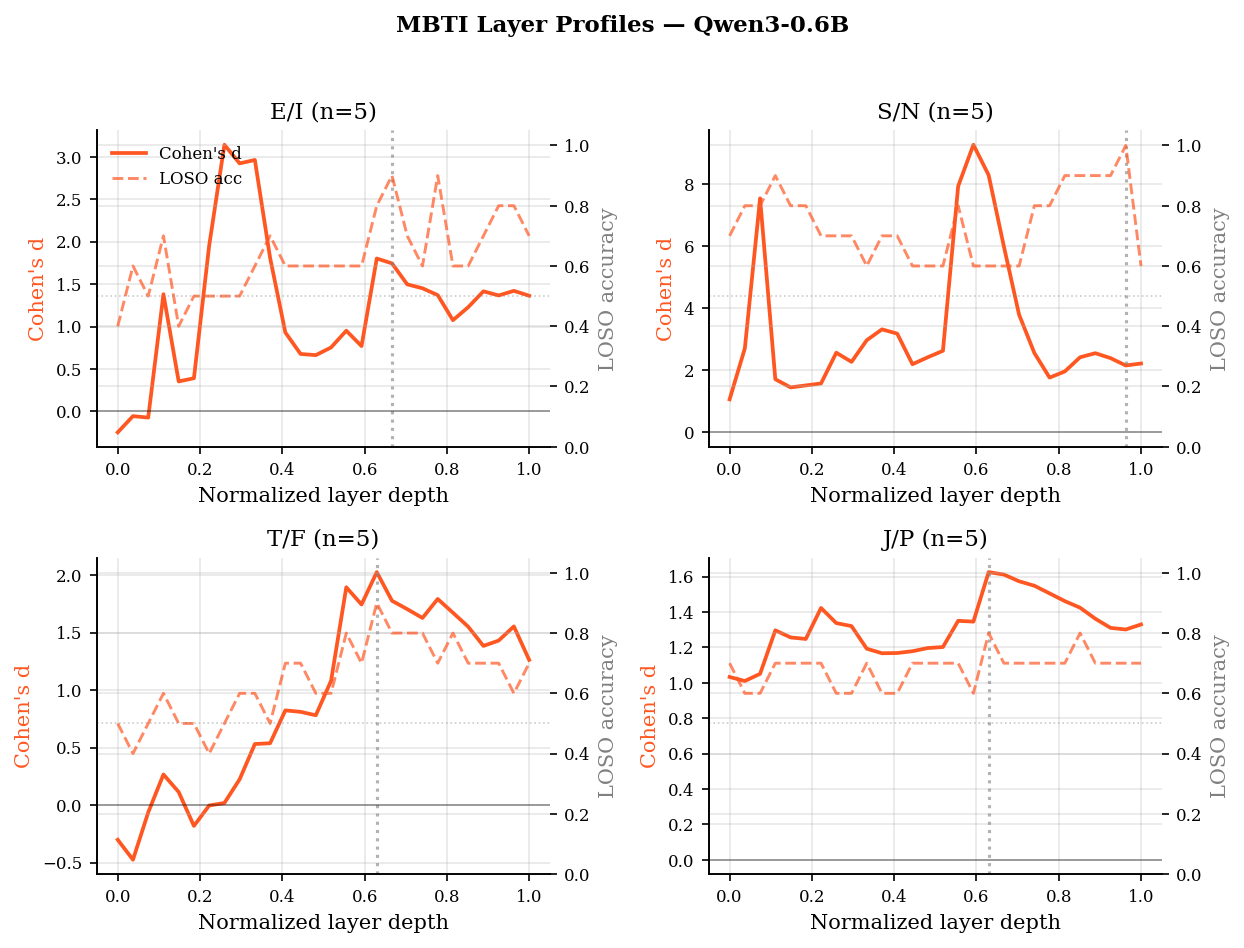
\includegraphics[width=\textwidth]{figures/layer_profile_Qwen_Qwen3-0.6B_mbti.png}
\caption{\textbf{Qwen3-0.6B: MBTI dimension layer profiles.}}
\label{fig:qwen3_mbti}
\end{figure}

\begin{figure}[H]
\centering
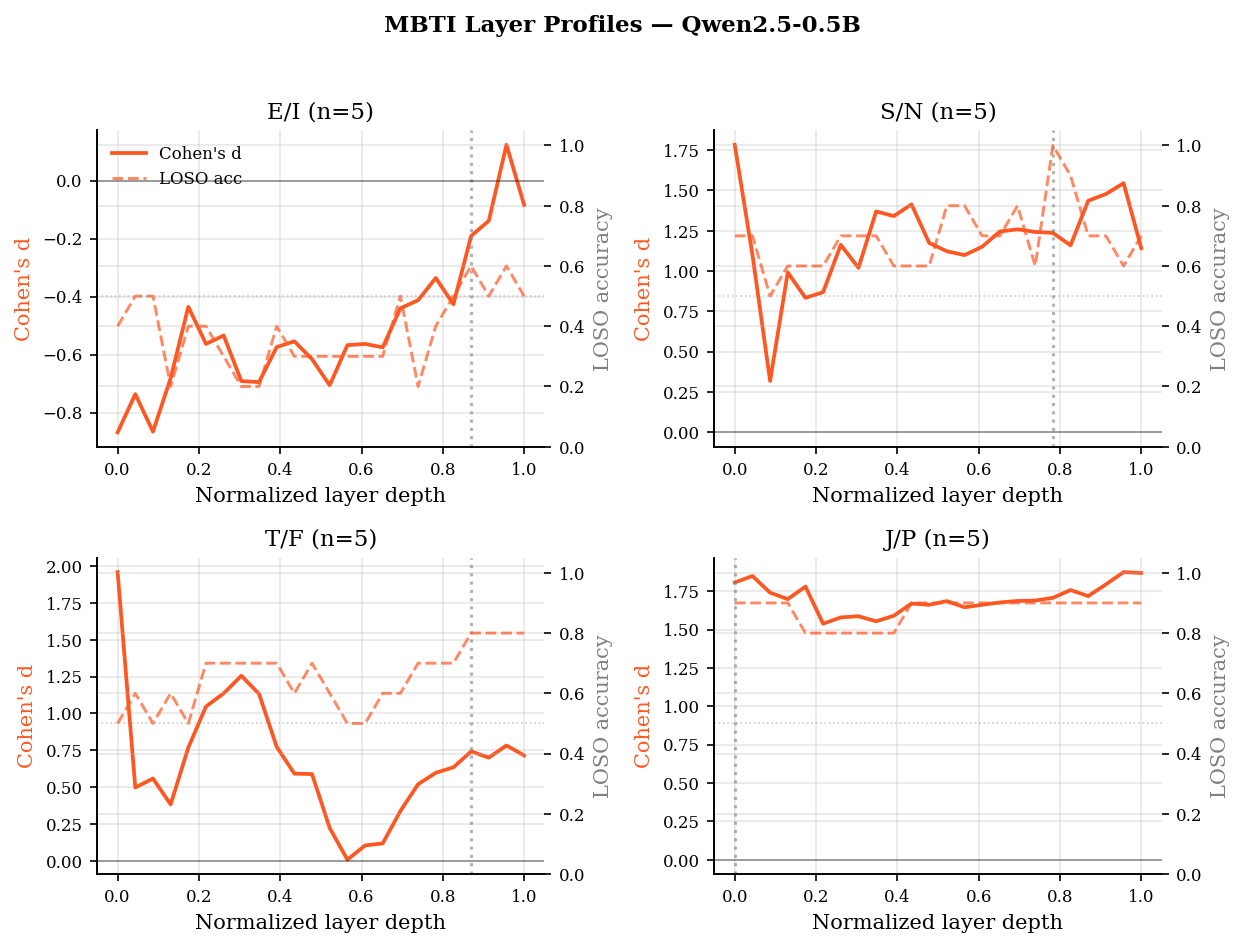
\includegraphics[width=\textwidth]{figures/layer_profile_Qwen_Qwen2.5-0.5B-Instruct_mbti.png}
\caption{\textbf{Qwen2.5-0.5B: MBTI dimension layer profiles.} The E/I subplot shows negative or near-zero d across all layers---the inversion anomaly.}
\label{fig:qwen25_mbti}
\end{figure}

\begin{figure}[H]
\centering
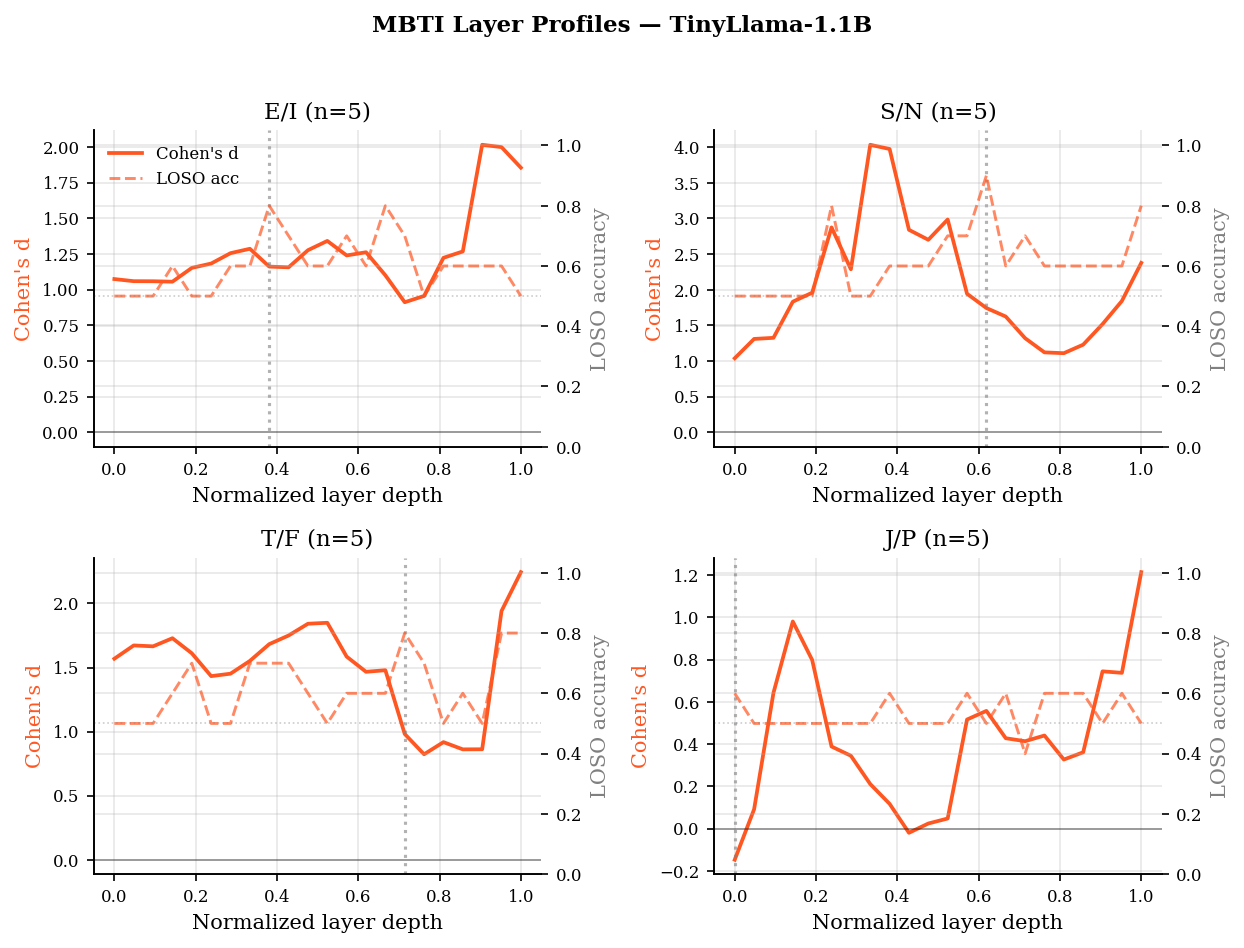
\includegraphics[width=\textwidth]{figures/layer_profile_TinyLlama_TinyLlama-1.1B-Chat-v1.0_mbti.png}
\caption{\textbf{TinyLlama-1.1B: MBTI dimension layer profiles.}}
\label{fig:tinyllama_mbti}
\end{figure}

\begin{figure}[H]
\centering
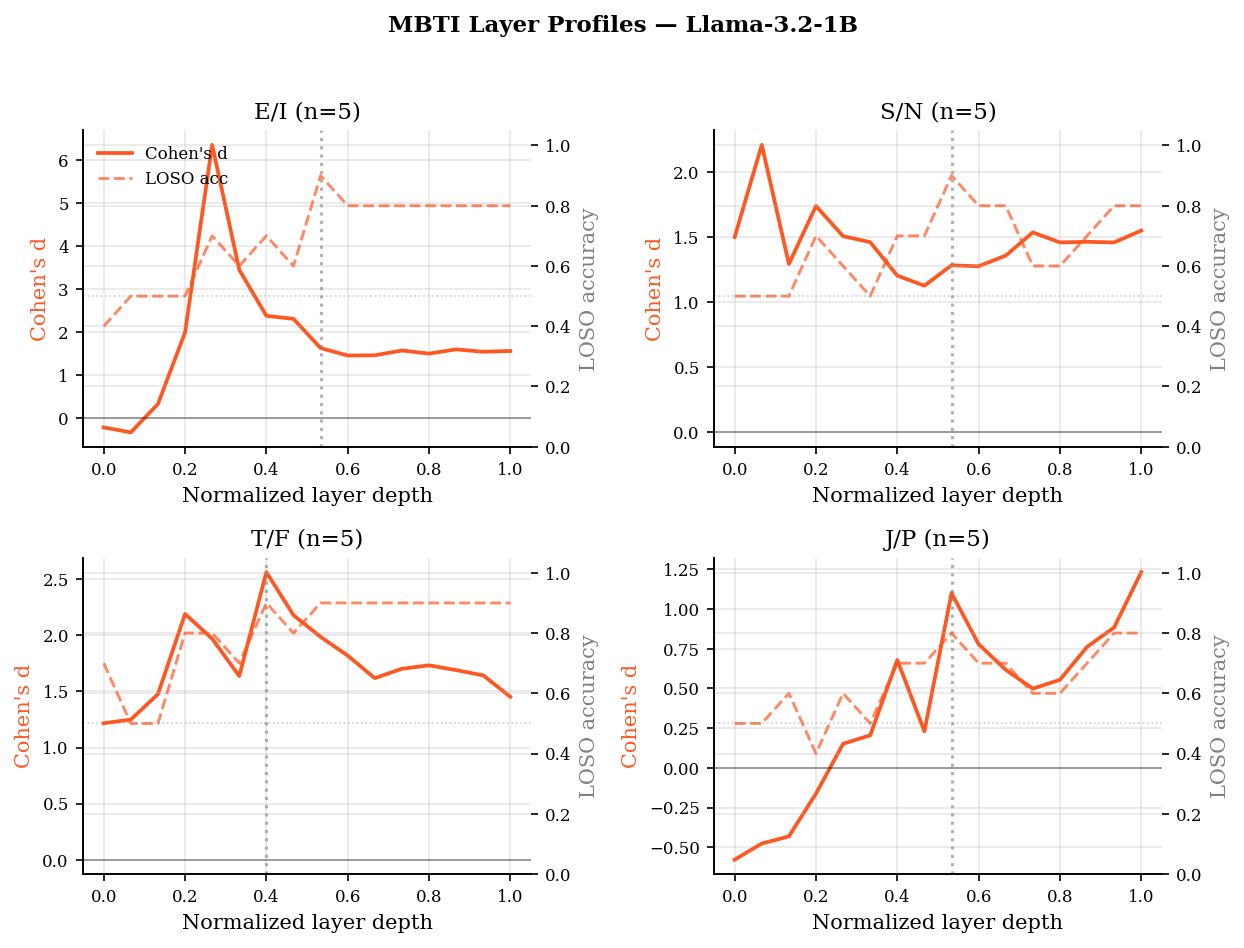
\includegraphics[width=\textwidth]{figures/layer_profile_unsloth_Llama-3.2-1B-Instruct_mbti.png}
\caption{\textbf{Llama-3.2-1B: MBTI dimension layer profiles.}}
\label{fig:llama32_mbti}
\end{figure}

\begin{figure}[H]
\centering
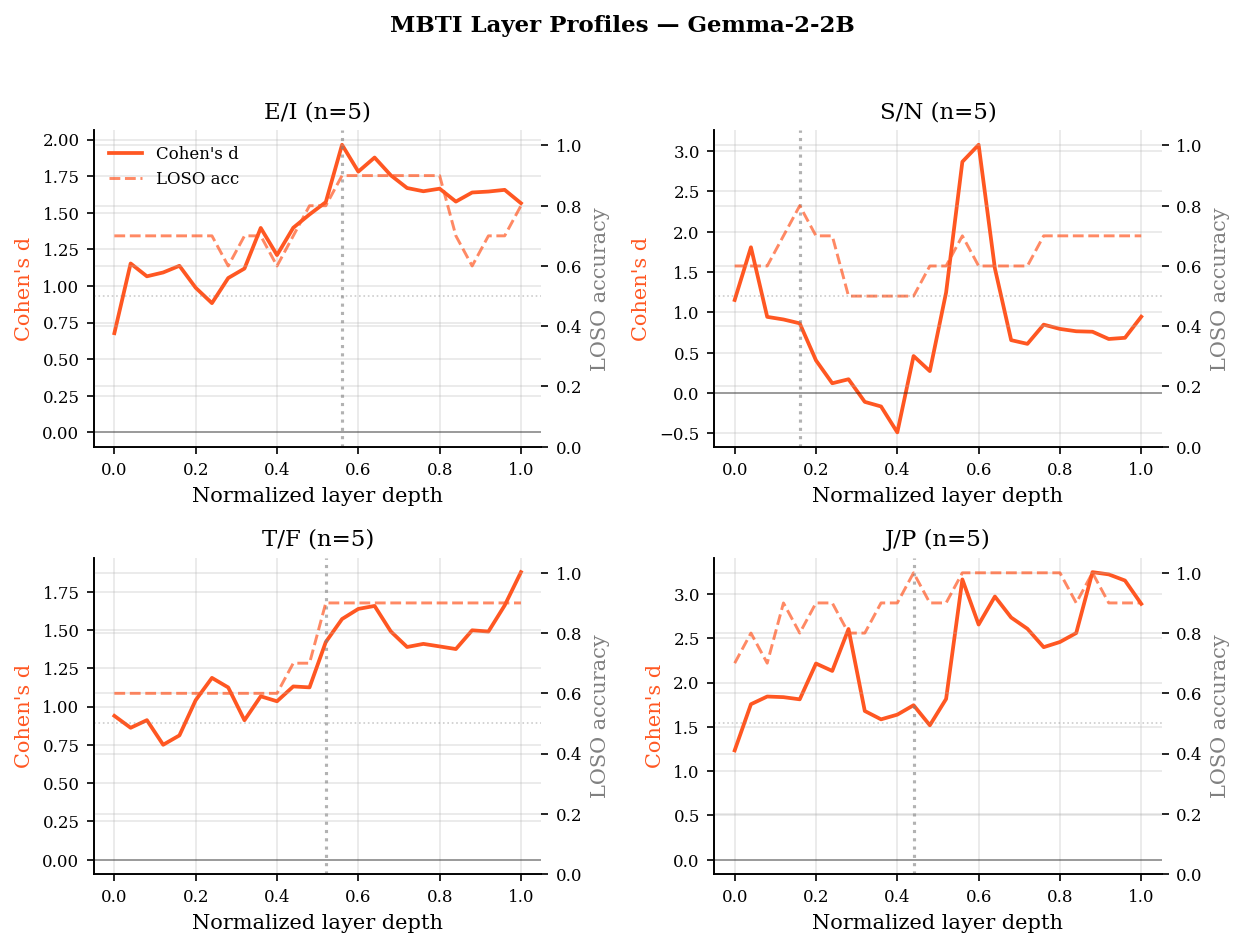
\includegraphics[width=\textwidth]{figures/layer_profile_unsloth_gemma-2-2b-it_mbti.png}
\caption{\textbf{Gemma-2-2B: MBTI dimension layer profiles.}}
\label{fig:gemma2_mbti}
\end{figure}

\clearpage

\subsection{Jungian Cognitive Function Layer Profiles by Model}

\begin{figure}[H]
\centering
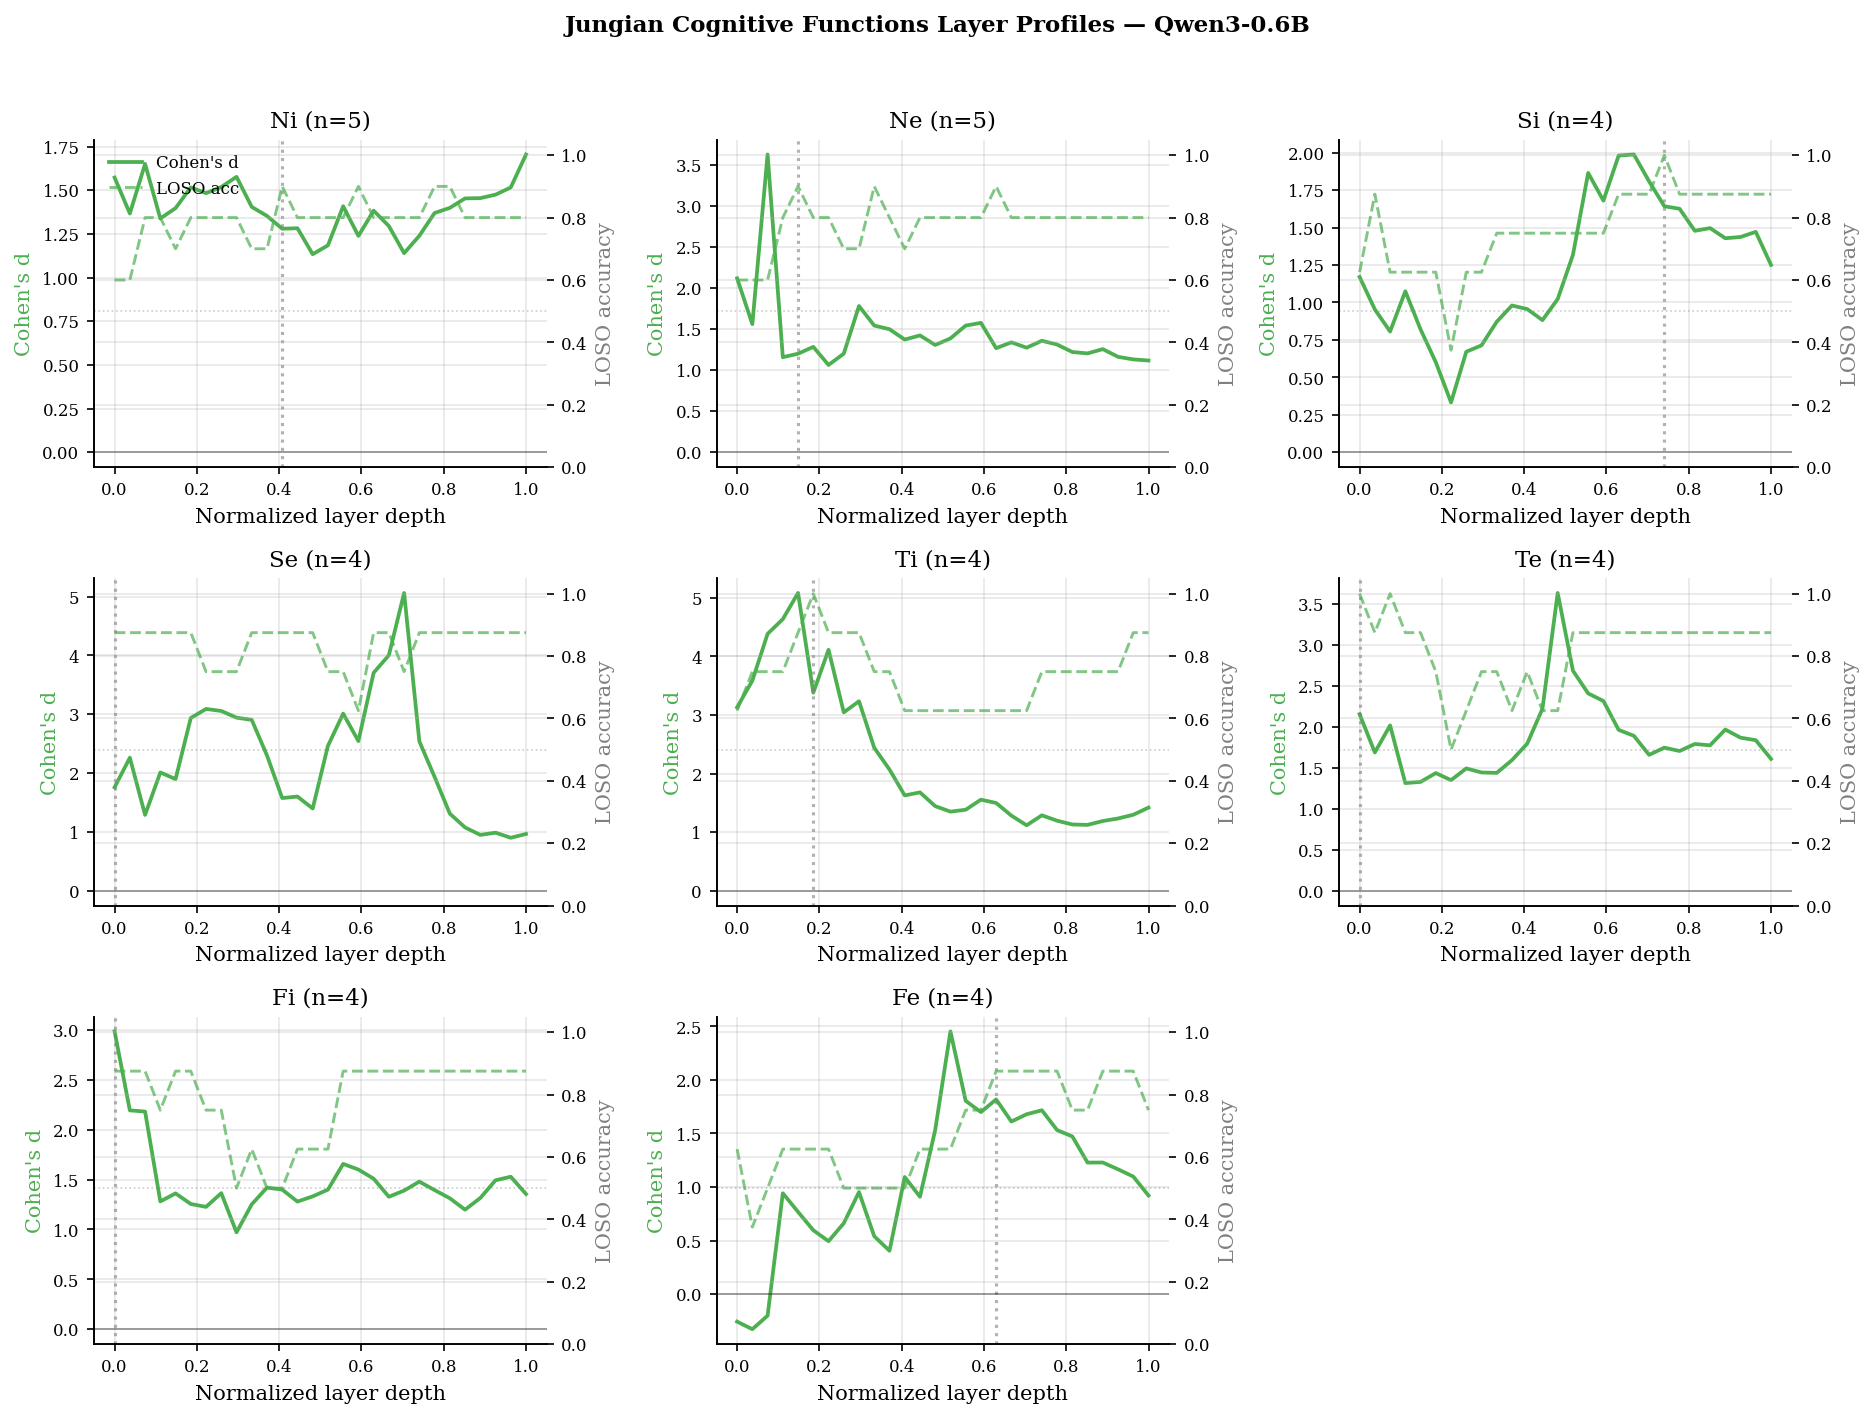
\includegraphics[width=\textwidth]{figures/layer_profile_Qwen_Qwen3-0.6B_jungian.png}
\caption{\textbf{Qwen3-0.6B: Jungian cognitive function layer profiles.} Ti and Fi peak sharply at the earliest layers (L0--L4); Te and Fe peak in middle layers; Ni uniquely peaks at the penultimate layer.}
\label{fig:qwen3_jungian}
\end{figure}

\begin{figure}[H]
\centering
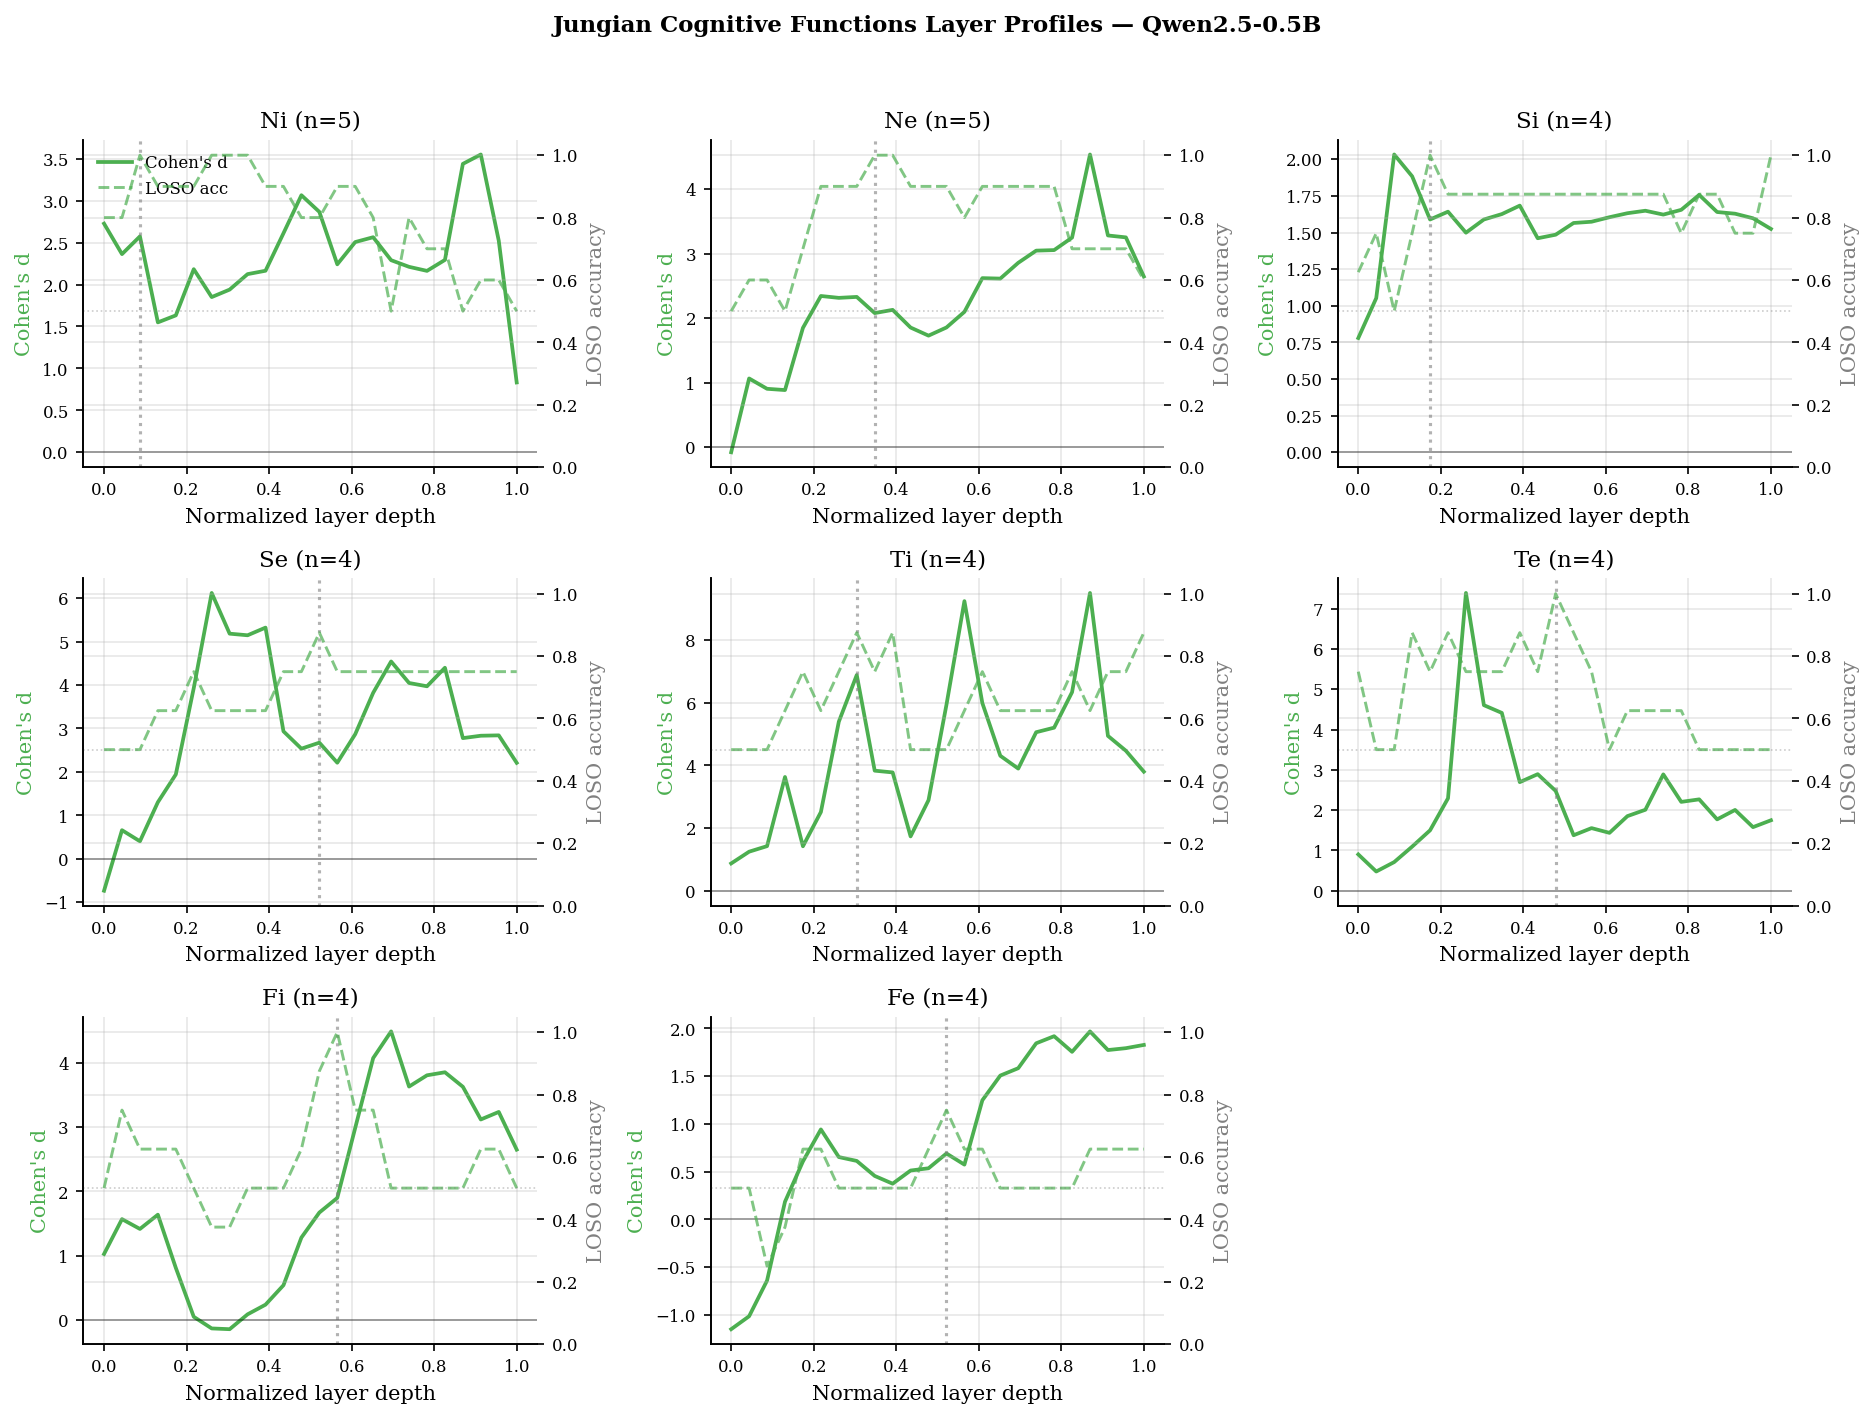
\includegraphics[width=\textwidth]{figures/layer_profile_Qwen_Qwen2.5-0.5B-Instruct_jungian.png}
\caption{\textbf{Qwen2.5-0.5B: Jungian cognitive function layer profiles.} Ti achieves an exceptionally high d=6.88 at an early layer.}
\label{fig:qwen25_jungian}
\end{figure}

\begin{figure}[H]
\centering
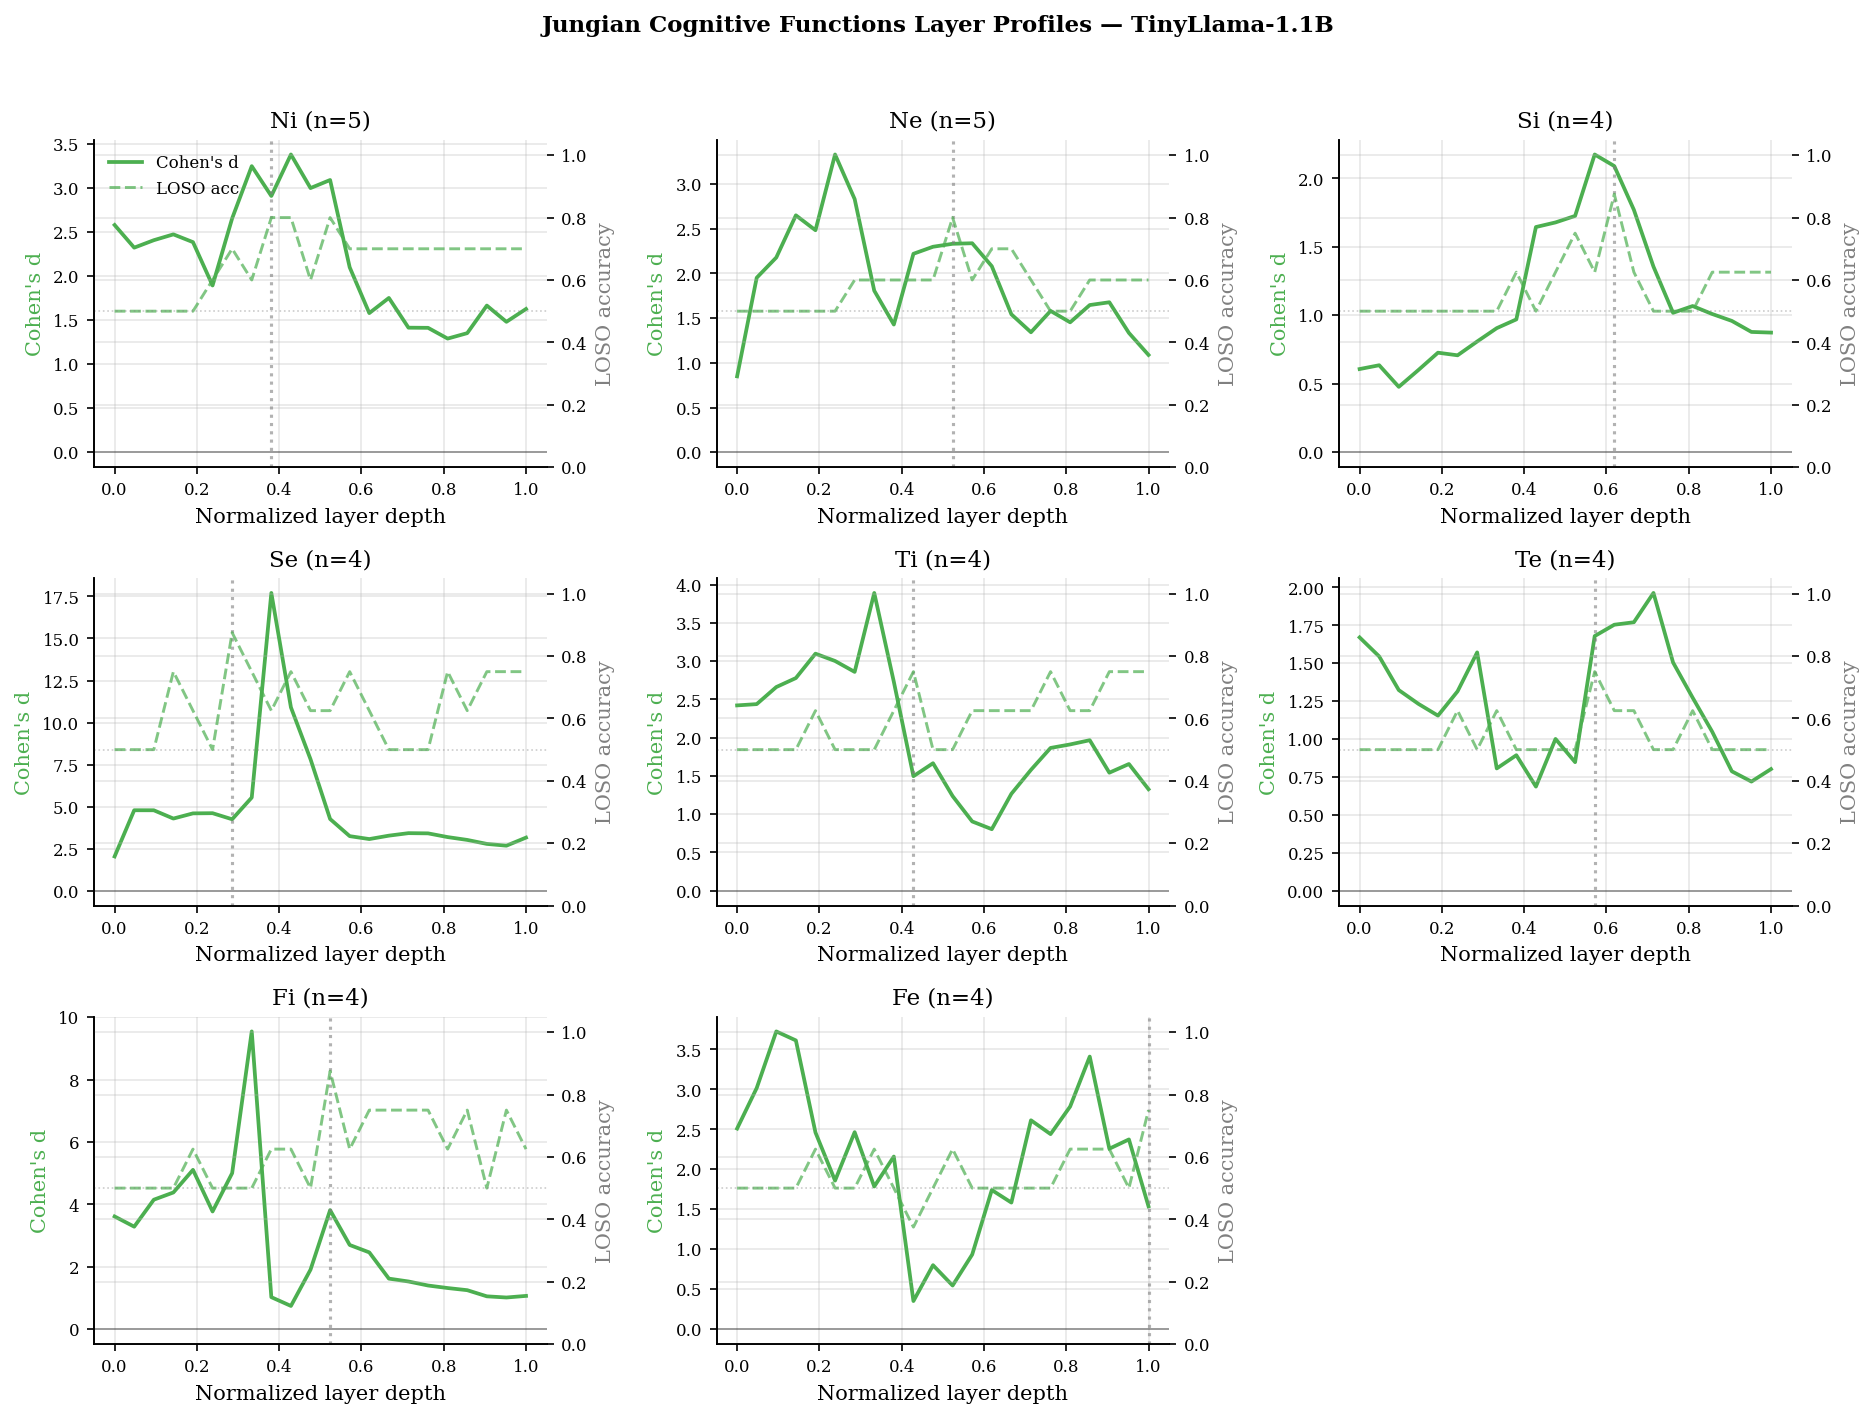
\includegraphics[width=\textwidth]{figures/layer_profile_TinyLlama_TinyLlama-1.1B-Chat-v1.0_jungian.png}
\caption{\textbf{TinyLlama-1.1B: Jungian cognitive function layer profiles.}}
\label{fig:tinyllama_jungian}
\end{figure}

\begin{figure}[H]
\centering
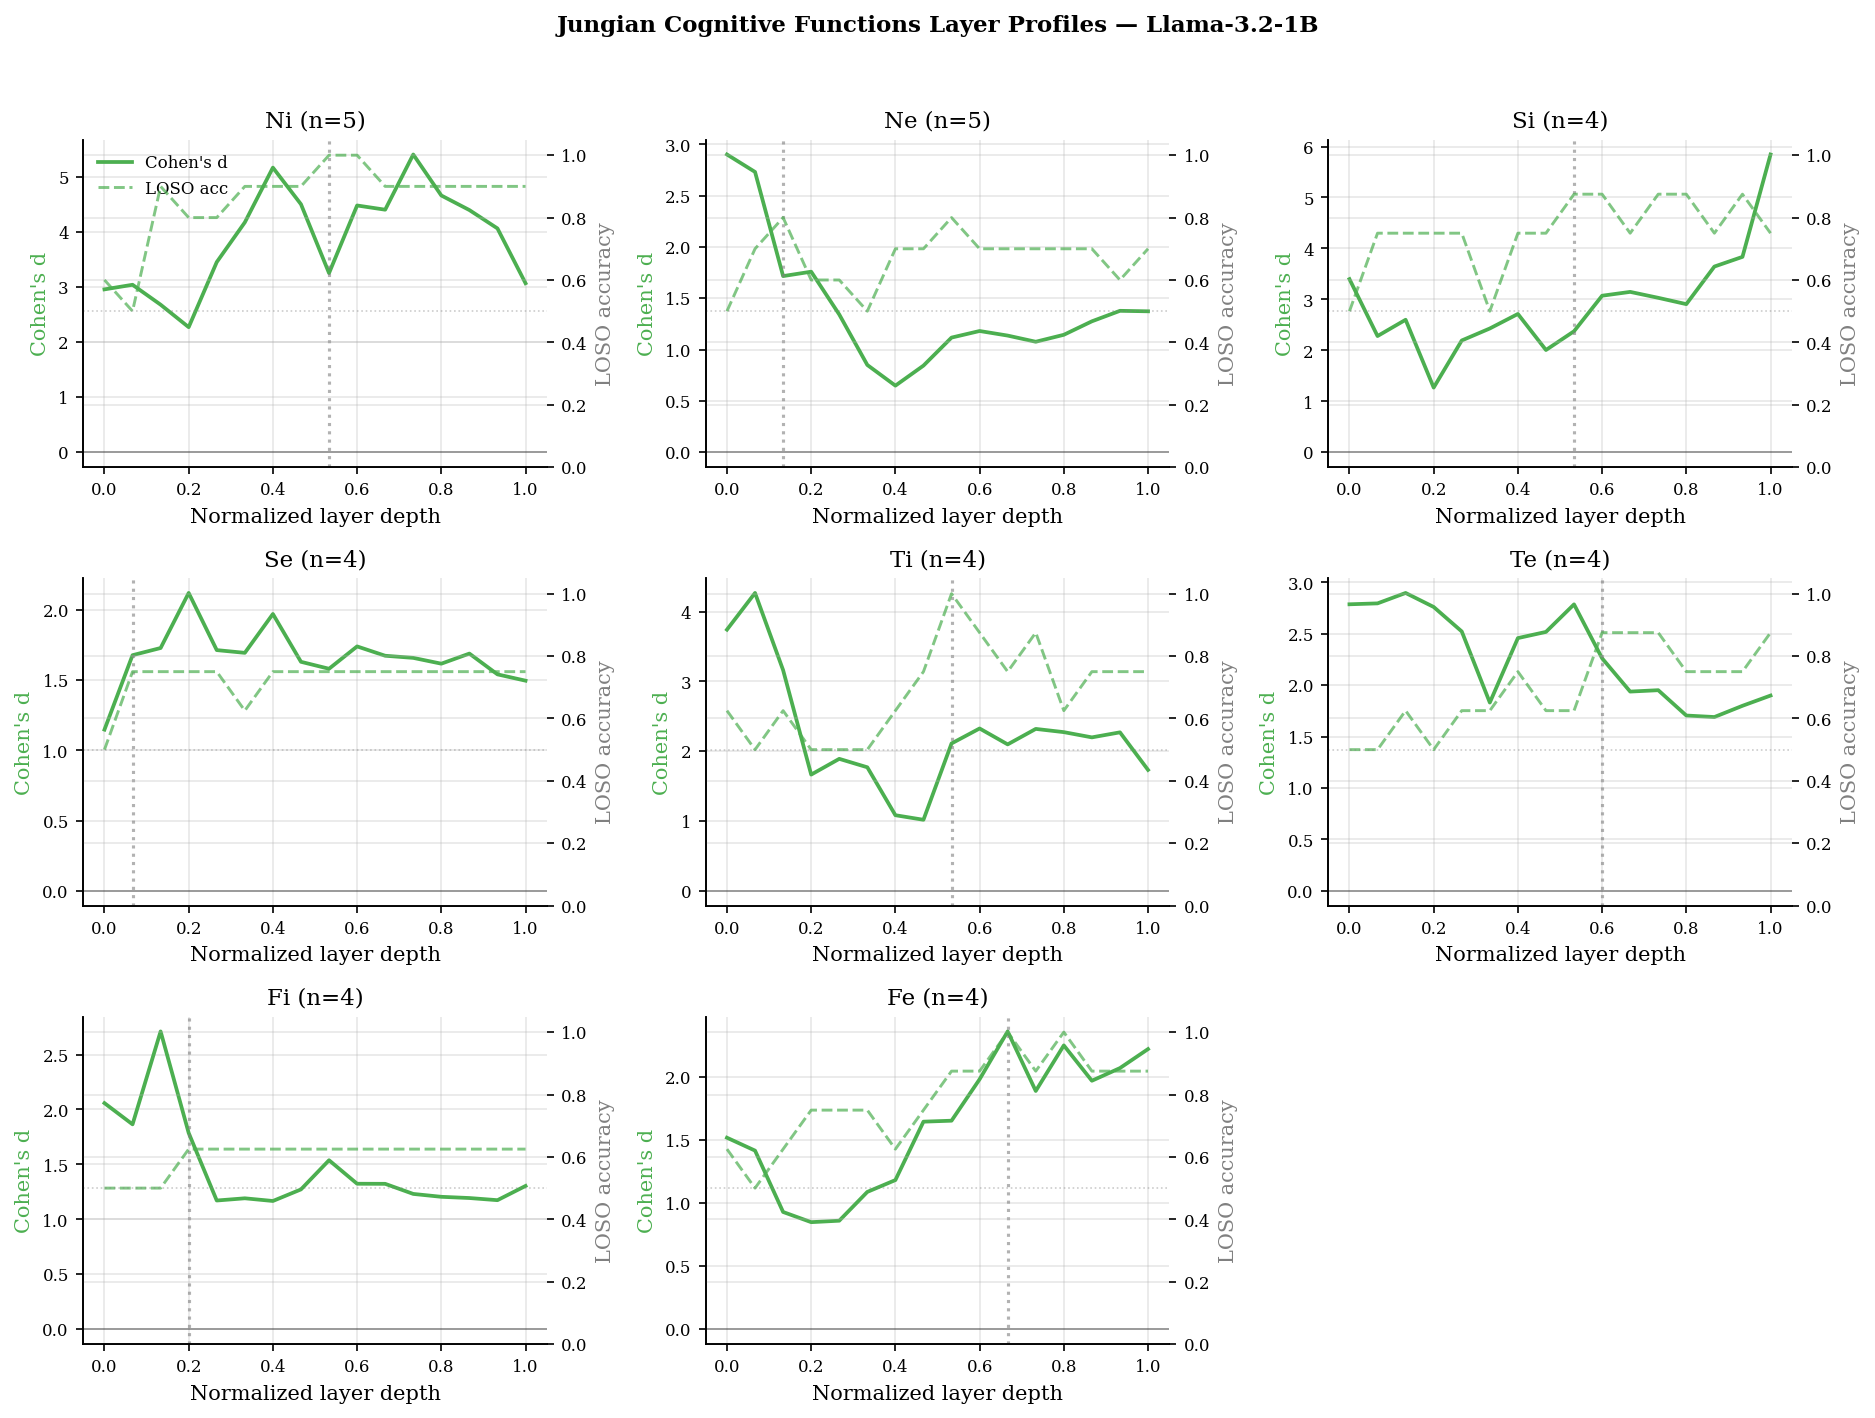
\includegraphics[width=\textwidth]{figures/layer_profile_unsloth_Llama-3.2-1B-Instruct_jungian.png}
\caption{\textbf{Llama-3.2-1B: Jungian cognitive function layer profiles.}}
\label{fig:llama32_jungian}
\end{figure}

\begin{figure}[H]
\centering
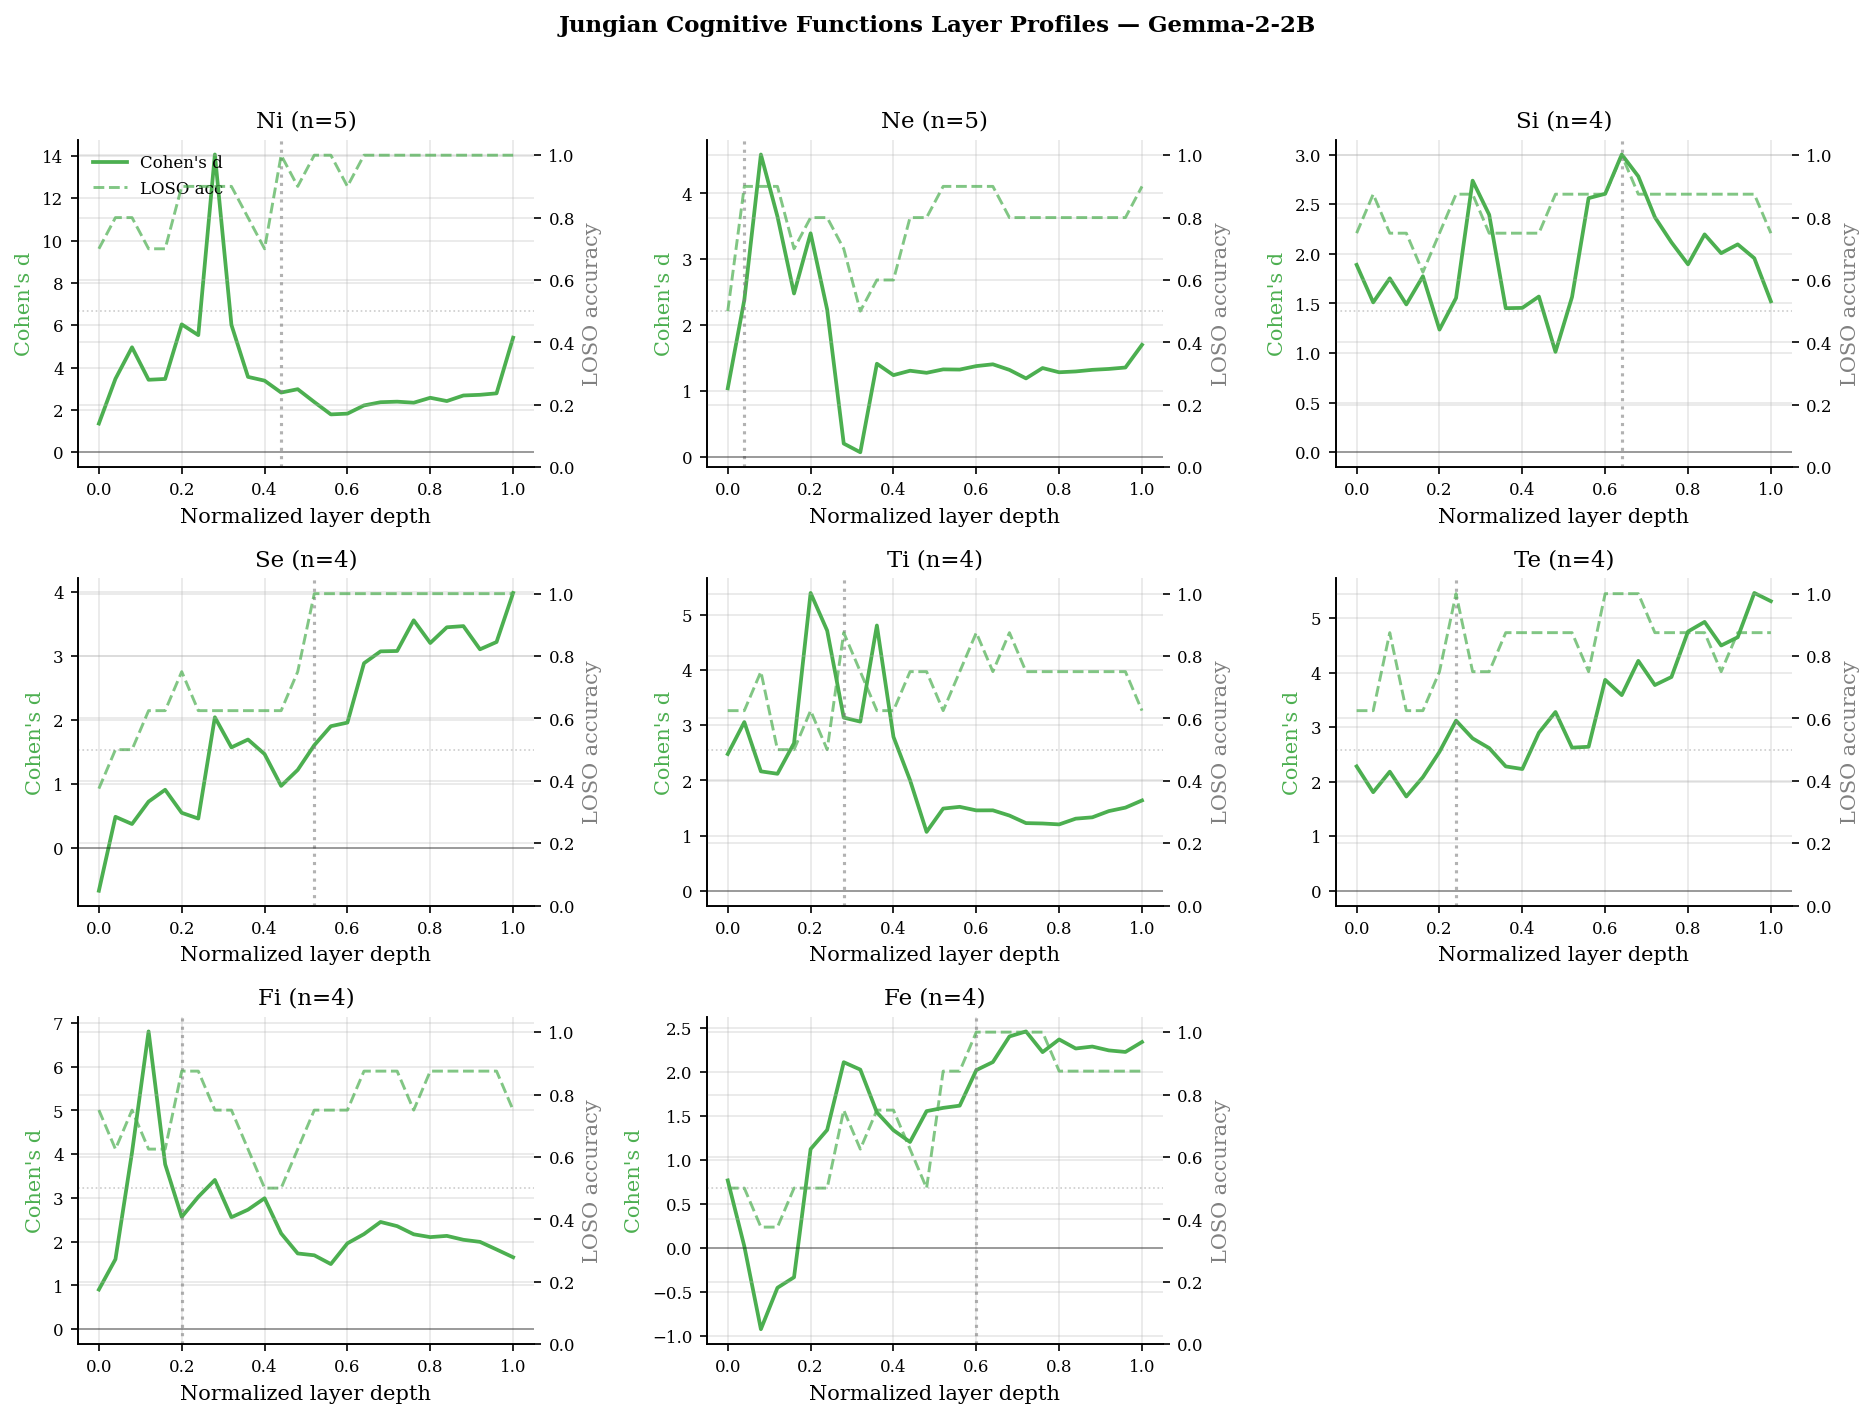
\includegraphics[width=\textwidth]{figures/layer_profile_unsloth_gemma-2-2b-it_jungian.png}
\caption{\textbf{Gemma-2-2B: Jungian cognitive function layer profiles.}}
\label{fig:gemma2_jungian}
\end{figure}

\clearpage

% ============================================================
\section{Control Experiments}\label{app:control}

\subsection{Position-Swap Control}\label{app:position_swap}

To address concerns that user-token causal dominance might reflect positional artifacts (recency effect), we reverse the prompt layout: placing the neutral scenario in the system role and the persona instruction in the user role.

Results reveal that causal influence remains concentrated at sequence-final positions regardless of content placement. This confirms a positional component consistent with the autoregressive bottleneck: the model's output distribution is most sensitive to activations nearest the generation point. However, early-layer specificity persists regardless of content placement, confirming attention-mediated propagation as the operative mechanism.

\subsection{Paraphrase Control}\label{app:paraphrase}

To rule out keyword confounding, we train probes on Template A (original prompts) and test on Template B (paraphrased versions), achieving 91.2\% mean cross-template accuracy (range: 87.5--100\%). Openness achieves perfect bidirectional transfer (1.000), confirming abstract conceptual representation rather than surface lexical cues.

\subsection{Out-of-Domain Generalization}\label{app:ood}

When extracting vectors from non-overlapping 50\% splits, OOD stability is strong for larger models (Llama-3.2 mean 0.988, Gemma-2 mean 0.914) and moderate for smaller models (Qwen2.5 mean 0.801). Openness shows exceptional stability (mean $\cos=0.935$), suggesting abstract conceptual encoding, while Extraversion and Agreeableness show context-dependent encoding.

% ============================================================
\section{Algorithm Pseudocode}\label{app:algorithm}

\begin{figure}[H]
\centering
\fbox{\parbox{0.92\textwidth}{\small
\textbf{Algorithm 1:} PersonaLens --- Standardized Personality Vector Extraction\\[4pt]
\textbf{Input:} Model $f_\theta$, Trait $t$, Contrastive pairs $\{(x^+_i, x^-_i)\}_{i=1}^K$\\
\textbf{Output:} Persona vectors $\{v_\ell\}_{\ell=0}^{L-1}$, Encoding profile, Causal map\\[4pt]
\textit{// Phase 2: Collect Activations}\\
1:\quad \textbf{for} $i = 1$ \textbf{to} $K$ \textbf{do}\\
2:\quad\quad $\{h_\ell(x^+_i)\}_{\ell=0}^{L-1} \leftarrow \text{ForwardPass}(f_\theta, x^+_i)$\\
3:\quad\quad $\{h_\ell(x^-_i)\}_{\ell=0}^{L-1} \leftarrow \text{ForwardPass}(f_\theta, x^-_i)$\\
4:\quad \textbf{end for}\\[4pt]
\textit{// Phase 3: Extract Vectors}\\
5:\quad \textbf{for} $\ell = 0$ \textbf{to} $L-1$ \textbf{do}\\
6:\quad\quad $v^{\text{diff}}_\ell \leftarrow \frac{1}{K}\sum_i [h_\ell(x^+_i) - h_\ell(x^-_i)]$ \hfill \textit{// Mean difference}\\
7:\quad\quad $w_\ell, a_\ell \leftarrow \text{LogisticRegression}(H^+_\ell, H^-_\ell)$ \hfill \textit{// Linear probe}\\
8:\quad\quad $u_\ell, \rho_\ell \leftarrow \text{PCA}(\{h_\ell(x^+_i) - h_\ell(x^-_i)\}_i)$ \hfill \textit{// PCA direction}\\
9:\quad \textbf{end for}\\[4pt]
\textit{// Phase 4: Causal Localization}\\
10:\quad \textbf{for} $\ell = 0$ \textbf{to} $L-1$ \textbf{do}\\
11:\quad\quad $\mathcal{I}(\ell) \leftarrow D_{\text{KL}}(\text{Clean}(x^+) \| \text{Patched}_\ell(x^+, h_\ell(x^-)))$\\
12:\quad \textbf{end for}\\
13:\quad \textbf{return} $\{v_\ell, a_\ell, \|v_\ell\|, \rho_\ell, \mathcal{I}(\ell)\}_\ell$
}}
\label{alg:personalens}
\end{figure}

% ============================================================
\section{Perplexity Calculation Methodology}\label{app:ppl}

\begin{equation}
\text{PPL} = \exp\left(-\frac{1}{T}\sum_{t=1}^{T} \log p_\theta(w_t | w_{<t})\right)
\end{equation}
where $p_\theta$ is the unmodified (un-steered) model's probability distribution. We compute perplexity on the \emph{full sequence} (prompt + generated response), using the base model without steering hooks active. The threshold of PPL $< 10$ was selected empirically: manual inspection revealed that outputs with PPL $> 10$ consistently exhibited token-level repetition loops, grammatical breakdown, or semantic incoherence. We acknowledge that absolute PPL values are not directly comparable across architectures due to different tokenizers and vocabulary sizes; the threshold serves as a within-model fluency gate rather than a cross-model metric.

\end{document}
